\documentclass[11pt, letterpaper]{article}\usepackage[]{graphicx}\usepackage[]{color}
% maxwidth is the original width if it is less than linewidth
% otherwise use linewidth (to make sure the graphics do not exceed the margin)
\makeatletter
\def\maxwidth{ %
  \ifdim\Gin@nat@width>\linewidth
    \linewidth
  \else
    \Gin@nat@width
  \fi
}
\makeatother

\definecolor{fgcolor}{rgb}{0.345, 0.345, 0.345}
\newcommand{\hlnum}[1]{\textcolor[rgb]{0.686,0.059,0.569}{#1}}%
\newcommand{\hlstr}[1]{\textcolor[rgb]{0.192,0.494,0.8}{#1}}%
\newcommand{\hlcom}[1]{\textcolor[rgb]{0.678,0.584,0.686}{\textit{#1}}}%
\newcommand{\hlopt}[1]{\textcolor[rgb]{0,0,0}{#1}}%
\newcommand{\hlstd}[1]{\textcolor[rgb]{0.345,0.345,0.345}{#1}}%
\newcommand{\hlkwa}[1]{\textcolor[rgb]{0.161,0.373,0.58}{\textbf{#1}}}%
\newcommand{\hlkwb}[1]{\textcolor[rgb]{0.69,0.353,0.396}{#1}}%
\newcommand{\hlkwc}[1]{\textcolor[rgb]{0.333,0.667,0.333}{#1}}%
\newcommand{\hlkwd}[1]{\textcolor[rgb]{0.737,0.353,0.396}{\textbf{#1}}}%
\let\hlipl\hlkwb

\usepackage{framed}
\makeatletter
\newenvironment{kframe}{%
 \def\at@end@of@kframe{}%
 \ifinner\ifhmode%
  \def\at@end@of@kframe{\end{minipage}}%
  \begin{minipage}{\columnwidth}%
 \fi\fi%
 \def\FrameCommand##1{\hskip\@totalleftmargin \hskip-\fboxsep
 \colorbox{shadecolor}{##1}\hskip-\fboxsep
     % There is no \\@totalrightmargin, so:
     \hskip-\linewidth \hskip-\@totalleftmargin \hskip\columnwidth}%
 \MakeFramed {\advance\hsize-\width
   \@totalleftmargin\z@ \linewidth\hsize
   \@setminipage}}%
 {\par\unskip\endMakeFramed%
 \at@end@of@kframe}
\makeatother

\definecolor{shadecolor}{rgb}{.97, .97, .97}
\definecolor{messagecolor}{rgb}{0, 0, 0}
\definecolor{warningcolor}{rgb}{1, 0, 1}
\definecolor{errorcolor}{rgb}{1, 0, 0}
\newenvironment{knitrout}{}{} % an empty environment to be redefined in TeX

\usepackage{alltt}
\usepackage[utf8]{inputenc}
\usepackage{amsmath}
\usepackage{xcolor}
\usepackage{geometry}
\usepackage[parfill]{parskip}
\usepackage{float}
\usepackage{graphicx}
\usepackage{fancyhdr}
\usepackage{appendix}
\graphicspath{{D:/Onedrive/__Projects/econforecasting/documentation-templates/images/}}
\newcommand{\vv}[1]{\textcolor{black}{\mathbf{#1}}}
\definecolor{econgreen}{RGB}{55, 91, 1}

\geometry{left=2.6cm, right = 2.6cm, top = 3cm, bottom = 3cm}

\fancypagestyle{plain}{
	\let\oldheadrule\headrule% Copy \headrule into \oldheadrule
	\renewcommand{\headrule}{\color{econgreen}\oldheadrule}
	\lhead{\small{\textcolor{black}{\leftmark}}}
	%\chead{}
	\rhead{\small{\textcolor{black}{\thepage}}}
	\lfoot{}
	\cfoot{}
	\rfoot{\textit{charles@cmefi.com}}
	\renewcommand{\headrulewidth}{0.5pt}
	%\renewcommand{\footrulewidth}{0.5pt}
}\pagestyle{plain}
\IfFileExists{upquote.sty}{\usepackage{upquote}}{}
\begin{document}
%%%%%%%%%%%%%%%%%%%%%%%%%%%%%%%%%%%%%%%%%%%%%%%%%%%%%%%%%%%%%%%%%%%%%
\begin{titlepage}
\thispagestyle{empty}
\newgeometry{left=5cm, top=5cm} %defines the geometry for the titlepage
\pagecolor{econgreen}
\noindent

\includegraphics[width=2cm]{cmefi_short.png} \\[-1em]
\color{white}
\makebox[0pt][l]{\rule{1.3\textwidth}{1pt}}
\par
\noindent
%\textbf{\textsf{A Macroeconomic Nowcasting Model}} 
%\vskip5cm
{\Huge \textsf{A Nowcasting Model for Time Series with Ragged-Edge Data}}
\vskip\baselineskip
\noindent
\textsf{Model Run Date: May 09, 2021}\\
\textsf{charles@cmefi.com}
\restoregeometry % restores the geometry
\nopagecolor% Use this to restore the color pages to white
\end{titlepage}
%%%%%%%%%%%%%%%%%%%%%%%%%%%%%%%%%%%%%%%%%%%%%%%%%%%%%%%%%%%%%%%%%%%%%%




\tableofcontents
\newpage
\listoftables
\listoffigures
\newpage
\section{Motivation}
\textbf{Nowcasting} is the prediction of the present, the near future, and the near past. Nowcasting is important in economics because many important macroeconomic statistics are released with a lengthy delay. For example, the Bureau of Economic Analysis releases quarterly GDP data typically two months after the quarter has already ended - a significant delay for any companies or individuals who need the data for planning and forecast models.

This delay is particularly salient during times of high volatility. During the first few months of the COVID-19 pandemic in the United States, many companies attempted to use high-frequency indicators to attempt nowcasts of the state of the macroeconomy. For example, a major investment bank forecasted Q2 GDP growth of -3\% on March 3rd; the estimate was revised down to -14\% by March 21st, -25\% by March 25th, and -40\% by April 10th. Yet many such models were ad-hoc and only able to use a small number of predictive indicators, such as jobless claims or traffic data.

\textbf{Nowcasting is about deciphering key information about the state of the economy before official data is released.} Because of the fundamentally urgent nature of nowcasting, it is important that nowcast models exploit any latest, high-frequency data available. Nowcasts should be able to generate constantly rolling forecasts, updating these numbers in response to any new data releases.


For example, suppose the date is early March, and the variable we want to predict is Q1 GDP. The simplest way to predict Q1 GDP would be to use historical quarterly data from various economic variables. But this data would only go up to Q4 of last year, and would fail to capture the critically important predictive power that could be provided by monthly and daily data released throughout January and February. This lag in publication dates of different data series is known as the \textbf{ragged-edge} problem.

Suppose instead, we used monthly data as our predictors of Q1 GDP. Again, we will soon run in to a problem. As an example, imagine that we had imported 20 monthly data series. Suppose 5 of these series ended in December, 10 ended in January, and 5 ended in March. 

\begin{figure}[H]
\caption{Example of ragged-edge data}
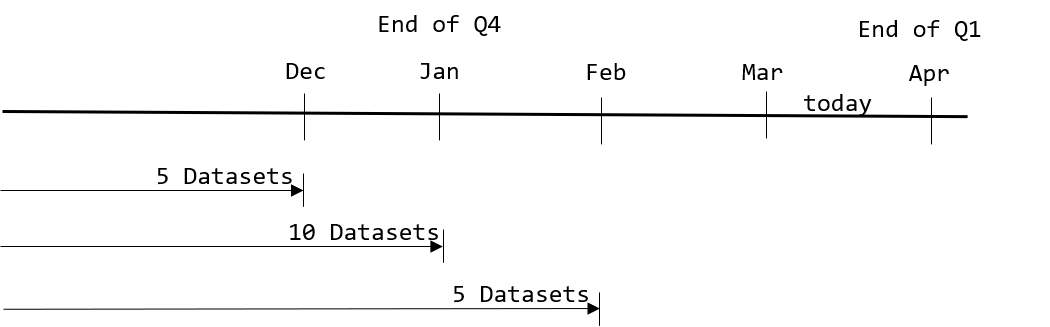
\includegraphics[scale=.7]{nowcast-time-2}
\centering
\end{figure}

Traditional modeling methods would require us to either throw out variables or throw out months - for example, we could truncate all our data series at January and lose out the information provided by the 5 February data points. Alternatively, we could completely remove the 15 variables with data releasing before March. Both methods result in a serious loss of useful data and are unappealing.

In this paper, we will develop and utilize a methodology that will allow us to use the information from \textbf{all variables} at \textbf{any dates}. This model will give an updated forecast in response to any new data releases. Additionally, the model can be generalized to nowcast any time series variable, not just GDP. The methodology for the model will be described in the next section.

\newpage
\section{Methodology Overview}
Our goal will be to take monthly-frequency leading economic predictor variables --- industrial production, consumer sentiment, vehicle sales, and so on --- and use these to predict our quarterly variables. However, we will need a way to adjust for the ragged edges of the data.

\begin{figure}[H]
\caption{Overview of methodology (more detail in later sections)}
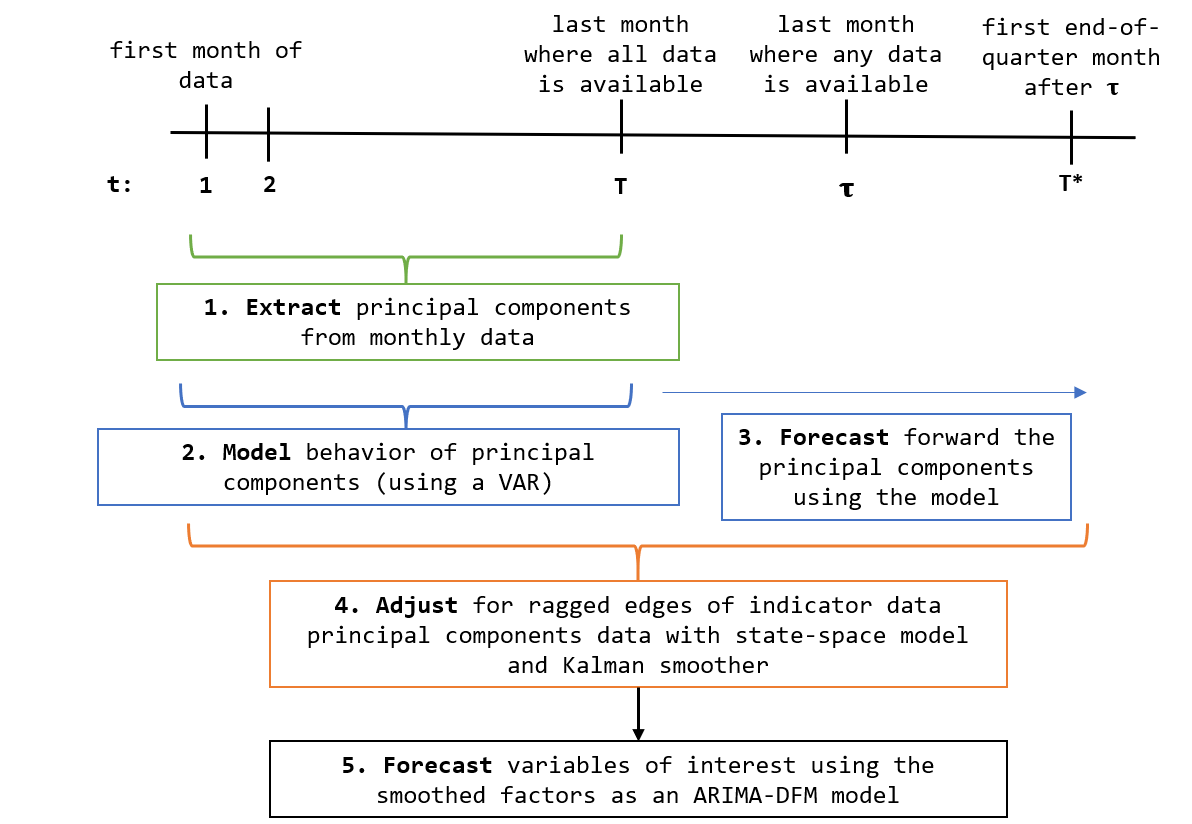
\includegraphics[scale=.7]{nowcast-time-3}
\centering
\end{figure}


To do this, we will use a methodology that relies heavily on principal components. It is well known that most macroeconomic variables are highly correlated with one another (see, for example, Bernanke et al 2005).
% latex table generated in R 4.0.4 by xtable 1.8-4 package
% Sun May 09 00:54:32 2021
\begin{table}[H]
\centering
\begingroup\scriptsize
\begin{tabular}{lrrrrrr}
  \hline
term & VehicleSales & ConsumerSentiment & AdvSales & IndustrialProd & VIX & SP500 \\ 
  \hline
VehicleSales &  &  &  &  &  &  \\ 
  ConsumerSentiment & 0.83 &  &  &  &  &  \\ 
  AdvSales & 0.12 & -0.14 &  &  &  &  \\ 
  IndustrialProd & 0.18 & -0.06 & 0.79 &  &  &  \\ 
  VIX & -0.58 & -0.53 & -0.08 & -0.23 &  &  \\ 
  SP500 & 0.10 & -0.00 & 0.55 & 0.40 & -0.64 &  \\ 
  CFNAI & 0.26 & -0.01 & 0.81 & 0.91 & -0.33 & 0.46 \\ 
   \hline
\end{tabular}
\endgroup
\caption{Correlation Between Major Leading Predictors} 
\end{table}

As a result, we can take a very high-dimensional dataset of indicator variables and extract a few time series, \textit{factors} or \textit{principal components}, using principal components analysis. These factors will be able to contain the majority of information within our larger, high-dimensional dataset. Then we will use a time series model of the factor behavior --- a vector autoregression, or VAR --- to forecast the factors forward in time. 

Finally, we will deal with the ragged edges of the data by casting our model dynamics in state-space form and using a Kalman filtration and smoothing process. This will, in essence, adjust our factor forecasts by whether or not the indicator variables used in the construction of the factors have been released. This procedure is a modified version of the two-step dynamic factor model utilized in Giannone et al (2008) and Doz et al (2011).

Finally, we will aggregate the smoothed and forecasted time series of factors up to a quarterly level. These now-quarterly forecasts of the factors can be used as covariates in an ARIMA model of the quarterly economic variables. The usage of factors as regressors of these economic variables is known as a \textit{dynamic factor model} (DFM). We additionally regularize our selection of regressors using a dynamic factor model.

The next section will go over the data and estimation procedure in detail. While this model can be generalized to nowcasts of other economic variables, we will use the example of nowcasting GDP and components of GDP.

\newpage
\section{Estimation Process}
The model is run every weekday; this documentation will use actual data and estimates from the most recent model run (2021-05-09) to illustrate the procedure. The final nowcasted output is located in the results section.

\subsection{Data}
We begin by importing monthly data of various leading indicators from the St. Louis Federal Reserve Database (FRED). We choose data of at least monthly frequency and with historical data available as of at least 2010. Data are transformed for stationarity as listed below; \textit{dlog} refers to the natural log of the first difference, whereas \textit{base} means that no transformation was necessary for the variable to be stationary.

% latex table generated in R 4.0.4 by xtable 1.8-4 package
% Sun May 09 00:54:32 2021
\begin{table}[H]
\centering
\begingroup\scriptsize
\begin{tabular}{lc}
  \hline
Variable & Stationary Form \\ 
  \hline
PCE & dlog \\ 
  Disposable Personal Income & dlog \\ 
  Case-Shiller Housing Price Index & dlog \\ 
  Housing Starts & dlog \\ 
  Houses Sold & dlog \\ 
  New Private Housing Permits & dlog \\ 
  Manufacturers New Orders: Durable Goods & dlog \\ 
  Capacity Utilization: Total Index & dlog \\ 
  Total Construction Spending & dlog \\ 
  Effective Federal Funds Rate & base \\ 
  Treasury Yield 10Y & base \\ 
  Treasury Yield 1Y & base \\ 
  Vehicle Sales & base \\ 
  Unemployment Rate & dlog \\ 
  Hires: Total Nonfarm & base \\ 
  Weekly Economic Index & base \\ 
  S\&P 500 & dlog \\ 
  VIX & base \\ 
  Crude Oil Price (West Texas Intermediate) & base \\ 
  Outstanding Real Estate Loans & dlog \\ 
  Outstanding Credit Card Balances & dlog \\ 
  St. Louis Fed Financial Stress Index & base \\ 
  U.S. Dollar Index & base \\ 
  Average Weeks Unemployed & base \\ 
  Retail \& Food Sales & dlog \\ 
  KC Fed Labor Market Index & base \\ 
  Consumer Confidence (OECD) & base \\ 
  Industrial Production index & dlog \\ 
  PCE Price Index & dlog \\ 
  New York Fed: Business Conditions Manufacturing Survey & base \\ 
  Dallas Fed: Current General Business Activity & base \\ 
  Philadelphia Fed: Future Capital Expenditures Survey & base \\ 
  Chicago Fed National Activity Index & base \\ 
  Baa Corporate Bond Yield & base \\ 
  Labor Force Participation Rate & base \\ 
   \hline
\end{tabular}
\endgroup
\caption{Imported Monthly Data - Leading Economic Variables} 
\end{table}


We additionally import quarterly data for our variables of interest. While this model can be used for nowcasting other data, here we will use import GDP, its components, as well as several other major macroeconomic variables of interest.
% latex table generated in R 4.0.4 by xtable 1.8-4 package
% Sun May 09 00:54:32 2021
\begin{table}[H]
\centering
\begingroup\scriptsize
\begin{tabular}{lc}
  \hline
Variable & Stationary Form \\ 
  \hline
GDP & dlog \\ 
  Consumption & dlog \\ 
  Consumption: Goods & dlog \\ 
  Consumption: Goods: Durable & dlog \\ 
  Consumption: Goods: Durable: Motor Vehicles \& Parts & dlog \\ 
  Consumption: Goods: Durable: Furnishings \& Durable Household Equipment & dlog \\ 
  Consumption: Goods: Durable: Recreational Goods \& Services & dlog \\ 
  Consumption: Goods: Durable: Other Durable Goods & dlog \\ 
  Consumption: Goods: Nondurable Goods & dlog \\ 
  Consumption: Goods: Nondurable Goods: Food \& Beverages for Off-Premises Use & dlog \\ 
  Consumption: Goods: Nondurable Goods: Clothing & dlog \\ 
  Consumption: Goods: Nondurable Goods: Gasoline \& Energy Goods & dlog \\ 
  Consumption: Goods: Nondurable Goods: Other Nondurable Goods & dlog \\ 
  Consumption: Services & dlog \\ 
  Consumption: Services: Housing \& Utilities & dlog \\ 
  Consumption: Services: Health Care & dlog \\ 
  Consumption: Services: Transportation & dlog \\ 
  Consumption: Services: Recreation & dlog \\ 
  Consumption: Services: Food Services \& Accomodations & dlog \\ 
  Consumption: Services: Financial Services & dlog \\ 
  Consumption: Services: Other Services & dlog \\ 
  Consumption: Services: Nonprofit Services & dlog \\ 
  Gross Private Domestic Investment & dlog \\ 
  Gross Private Domestic Investment: Nonresidential Investment & dlog \\ 
  Gross Private Domestic Investment: Nonresidential Investment: Structures & dlog \\ 
  Gross Private Domestic Investment: Nonresidential Investment: Equipment & dlog \\ 
  Gross Private Domestic Investment: Nonresidential Investment: Intellectual Property & dlog \\ 
  Gross Private Domestic Investment: Residential Investment & dlog \\ 
  Gross Private Domestic Investment: Change in Private Inventories & base \\ 
  Net Exports & base \\ 
  Exports & dlog \\ 
  Exports: Exported Goods & dlog \\ 
  Exports: Exported Services & dlog \\ 
  Imports & dlog \\ 
  Imports: Imported Goods & dlog \\ 
  Imports: Imported Services & dlog \\ 
  Government Spending & dlog \\ 
  Government Spending: Federal & dlog \\ 
  Government Spending: State \& Local & dlog \\ 
  Delinquency Rate on Residential Mortgages & base \\ 
  Delinquency Rate on Credit Cards & base \\ 
  Delinquency Rate on Commercial \& Industrial Loans & base \\ 
   \hline
\end{tabular}
\endgroup
\caption{Imported Quarterly Data} 
\end{table}


Finally, we import additional monthly data that may be of interest to forecast, but are not leading indicators that we will use in our principal components analysis.
% latex table generated in R 4.0.4 by xtable 1.8-4 package
% Sun May 09 00:54:32 2021
\begin{table}[H]
\centering
\begingroup\scriptsize
\begin{tabular}{lc}
  \hline
Variable & Stationary Form \\ 
  \hline
\hline
\end{tabular}
\endgroup
\caption{Other Imported Monthly Data} 
\end{table}


Most datasets have already been deseasonalized if necessary by their original source. We deseasonalize the remaining series by using the U.S. Census Bureau's seasonal adjustment package, X13-ARIMA-SEATS. We interface with it by using the \texttt{seasonal} package implementation in R (Sax and Eddelbuettel 2018).

\subsection{Time Periods}
Now we will segment the data by time periods. The imported monthly data will have ragged edges - i.e., some monthly data will be available for later months than others.

We will let $T$ denote the number of dates for which data is available for all data series. $\tau$ will denote the number of dates for which data is available for at least one data series. $T^*$ will denote number of dates up to the end-of-quarter month of the $\tau$ date. For example, suppose date $\tau$ occurs on February. The end-of-quarter month, $T^*$, will be March (since Q1 runs through the end of March). 

In other words, data will be indexed by $t = 1, 2, \dots, T, T+1, \dots, \tau, \dots, T^*$, where dates $T + 1$ through $\tau$ are the dates for which only some data are available, and dates $\tau + 1$ through $T^*$ are the dates for which no data is available up to the next quarter-ending month.
\begin{figure}[H]
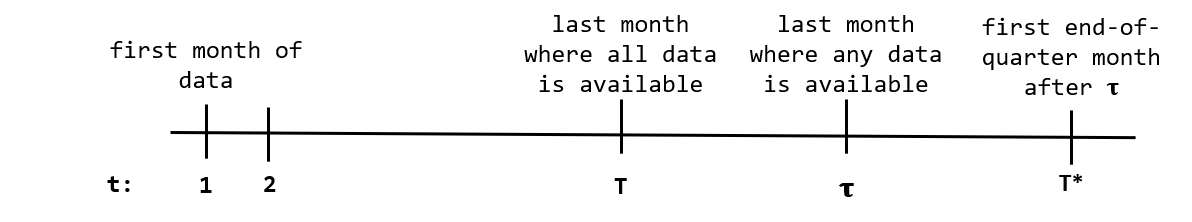
\includegraphics[scale=.7]{nowcast-time}
\centering
\end{figure}
For our data, we set the dates as follows.
% latex table generated in R 4.0.4 by xtable 1.8-4 package
% Sun May 09 00:54:32 2021
\begin{table}[H]
\centering
\begingroup\footnotesize
\begin{tabular}{cc}
  \hline
Date & $t$ \\ 
  \hline
2010-01-01 & $1$ \\ 
  2021-02-01 & $T$ \\ 
  2021-05-01 & $\tau$ \\ 
  2021-05-01 & $T*$ \\ 
   \hline
\end{tabular}
\endgroup
\caption{Time Periods} 
\end{table}


\subsection{Principal Components Analysis}
It is known that a large number of macroeconomic time series are highly correlated; using such covariates as regressors could naturally lead to problems with collinearity and unstable estimates. In addition, it becomes computationally burdensome to analyze data with such a large number of highly correlated variables. Instead, we use principal components analysis (PCA) to shrink our dataset in a way that allows us to retain most of the information in our original data.

Estimation of factors is derived following Stock and Watson (2008). We begin by taking our $T \times N$ data matrix of $N$ monthly leading economic variables, from time 1 through $T$. The matrix, which we denote $X$, is normalized to mean 0 and variance 0 across all columns.

The goal is to minimize the error $E$ below.
\begin{align*}
	X = F  \Lambda ' + E,\\
	\text{where $X$ is the $T \times N$ data matrix,}\\
	\text{$F$ is the $T \times N$ matrix of factors,}\\
	\text{and $\Lambda$ is the weighting matrix.}\\
\end{align*}

Estimation of factors is derived following Stock and Watson (2008).
\begin{align*}
	\widehat{\Lambda} = \text{eigenvectors of } (X'X)\\
	\widehat{F} = X \widehat{\Lambda}
\end{align*}



Once factors are derived, we select the optimal number of factors to use in predictive regressions. To do so, we use the information criteria from Bai and Ng (2002). Let $R$ refer to the number of factors used. We also include alternative specifications of the information criteria from Bai and Ng as a robustness check.
\begin{align*}
	IC(R) = MSE + R \times \frac{N+T}{NT} \times log\left(\frac{NT}{N+T}\right)
\end{align*}

\begin{figure}[H]

{\centering 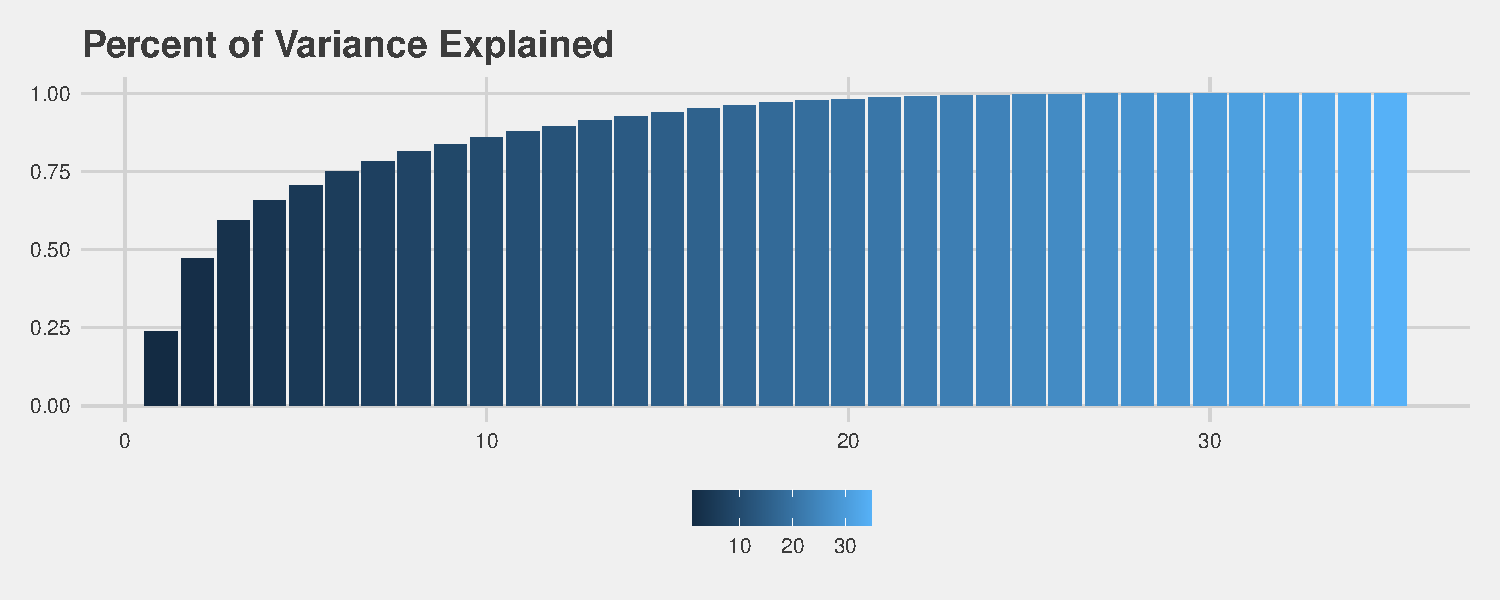
\includegraphics[width=5in,height=2in]{D:/Onedrive/__Projects/econforecasting/model-outputs/latex-figures/unnamed-chunk-8-1} 

}

\caption[Factor Selection]{Factor Selection}\label{fig:unnamed-chunk-8}
\end{figure}



% latex table generated in R 4.0.4 by xtable 1.8-4 package
% Sun May 09 00:54:32 2021
\begin{table}[H]
\centering
\begingroup\scriptsize
\begin{tabular}{cccccccc}
  \hline
Factors (R) & Variance Explained & Pct of Total Var Explained & Cumulative Pct & MSE & IC1 & IC2 & IC3 \\ 
  \hline
  1 & 8.33 & 0.24 & 0.24 & 0.76 & 0.88 & 0.88 & 0.86 \\ 
    2 & 8.13 & 0.23 & 0.47 & 0.53 & 0.77 & 0.78 & 0.73 \\ 
    3 & 4.31 & 0.12 & 0.59 & 0.40 & 0.76 & 0.79 & 0.71 \\ 
    4 & 2.18 & 0.06 & 0.66 & 0.34 & 0.82 & 0.85 & 0.75 \\ 
    5 & 1.75 & 0.05 & 0.71 & 0.29 & 0.89 & 0.93 & 0.80 \\ 
    6 & 1.53 & 0.04 & 0.75 & 0.25 & 0.97 & 1.02 & 0.86 \\ 
    7 & 1.15 & 0.03 & 0.78 & 0.22 & 1.06 & 1.11 & 0.93 \\ 
    8 & 1.04 & 0.03 & 0.81 & 0.19 & 1.15 & 1.21 & 1.00 \\ 
    9 & 0.83 & 0.02 & 0.84 & 0.16 & 1.24 & 1.32 & 1.08 \\ 
   10 & 0.77 & 0.02 & 0.86 & 0.14 & 1.34 & 1.42 & 1.16 \\ 
   11 & 0.66 & 0.02 & 0.88 & 0.12 & 1.44 & 1.53 & 1.24 \\ 
   12 & 0.62 & 0.02 & 0.89 & 0.10 & 1.54 & 1.64 & 1.32 \\ 
   13 & 0.59 & 0.02 & 0.91 & 0.09 & 1.65 & 1.76 & 1.41 \\ 
   14 & 0.50 & 0.01 & 0.93 & 0.07 & 1.75 & 1.87 & 1.50 \\ 
   15 & 0.49 & 0.01 & 0.94 & 0.06 & 1.86 & 1.98 & 1.58 \\ 
   16 & 0.43 & 0.01 & 0.95 & 0.05 & 1.97 & 2.10 & 1.67 \\ 
   17 & 0.34 & 0.01 & 0.96 & 0.04 & 2.08 & 2.22 & 1.76 \\ 
   18 & 0.25 & 0.01 & 0.97 & 0.03 & 2.19 & 2.34 & 1.86 \\ 
   19 & 0.24 & 0.01 & 0.98 & 0.02 & 2.30 & 2.46 & 1.95 \\ 
   20 & 0.20 & 0.01 & 0.98 & 0.02 & 2.42 & 2.58 & 2.05 \\ 
   21 & 0.15 & 0.00 & 0.99 & 0.01 & 2.53 & 2.71 & 2.15 \\ 
   22 & 0.13 & 0.00 & 0.99 & 0.01 & 2.65 & 2.83 & 2.25 \\ 
   23 & 0.10 & 0.00 & 0.99 & 0.01 & 2.76 & 2.96 & 2.34 \\ 
   24 & 0.07 & 0.00 & 0.99 & 0.01 & 2.88 & 3.09 & 2.44 \\ 
   25 & 0.06 & 0.00 & 1.00 & 0.00 & 3.00 & 3.21 & 2.54 \\ 
   26 & 0.04 & 0.00 & 1.00 & 0.00 & 3.12 & 3.34 & 2.64 \\ 
   27 & 0.03 & 0.00 & 1.00 & 0.00 & 3.24 & 3.47 & 2.75 \\ 
   28 & 0.03 & 0.00 & 1.00 & 0.00 & 3.36 & 3.59 & 2.85 \\ 
   29 & 0.02 & 0.00 & 1.00 & 0.00 & 3.48 & 3.72 & 2.95 \\ 
   30 & 0.01 & 0.00 & 1.00 & 0.00 & 3.60 & 3.85 & 3.05 \\ 
   31 & 0.01 & 0.00 & 1.00 & 0.00 & 3.72 & 3.98 & 3.15 \\ 
   32 & 0.01 & 0.00 & 1.00 & 0.00 & 3.84 & 4.11 & 3.25 \\ 
   33 & 0.01 & 0.00 & 1.00 & 0.00 & 3.96 & 4.23 & 3.35 \\ 
   34 & 0.00 & 0.00 & 1.00 & 0.00 & 4.08 & 4.36 & 3.45 \\ 
   35 & 0.00 & 0.00 & 1.00 & 0.00 & 4.20 & 4.49 & 3.56 \\ 
   \hline
\end{tabular}
\endgroup
\caption{Factor Selection Process} 
\end{table}


Choosing the IC-minimizing $R$ lets us choose $R = 2$ factors.



{\centering 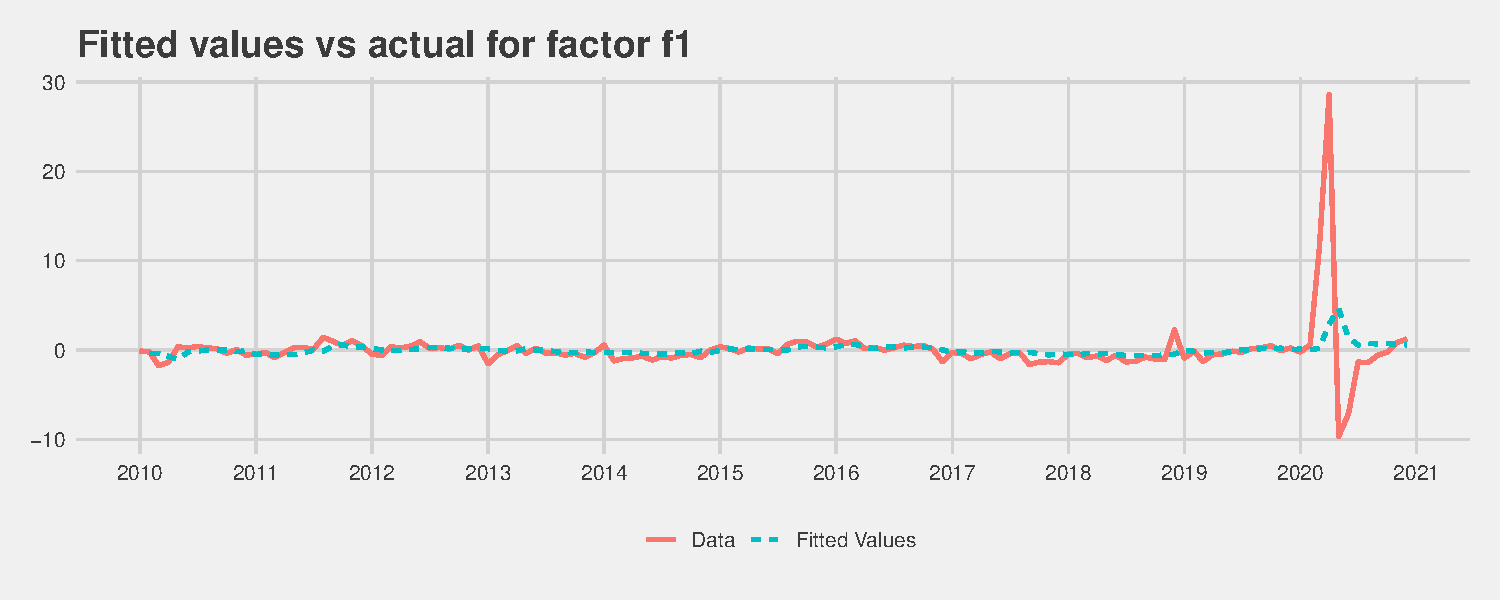
\includegraphics[width=5in,height=2in]{D:/Onedrive/__Projects/econforecasting/model-outputs/latex-figures/unnamed-chunk-10-1} 

}




{\centering 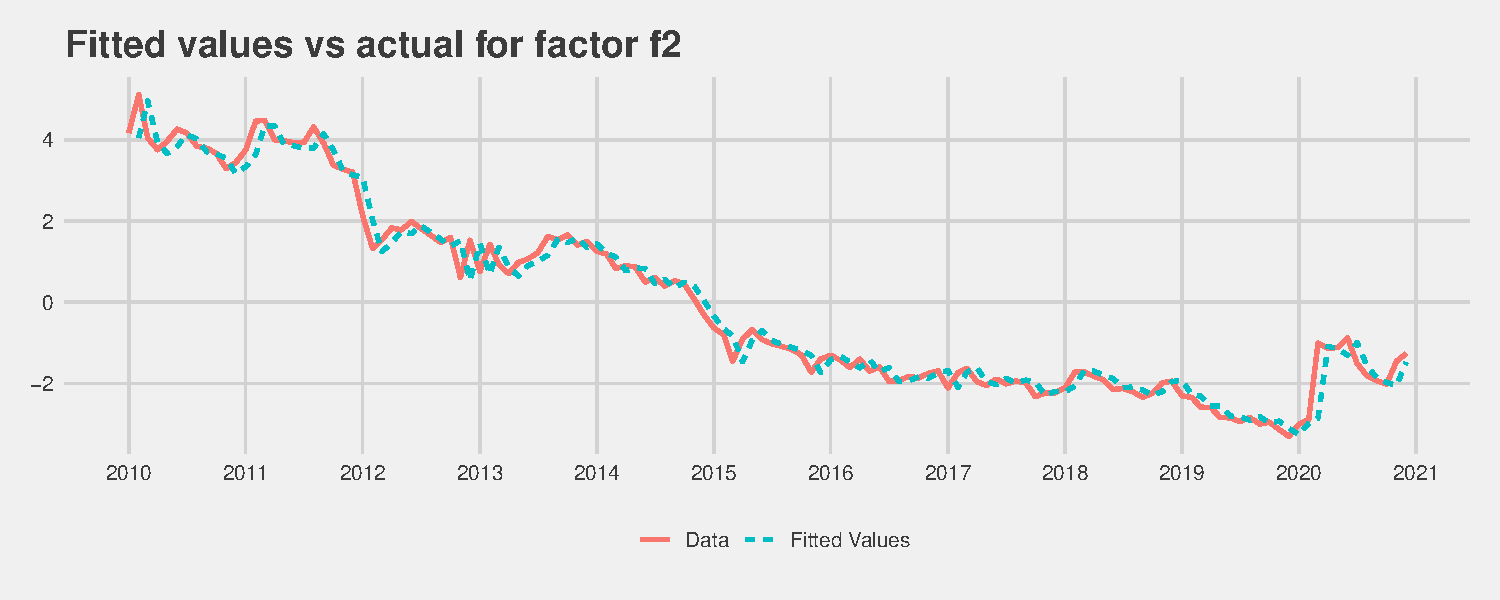
\includegraphics[width=5in,height=2in]{D:/Onedrive/__Projects/econforecasting/model-outputs/latex-figures/unnamed-chunk-10-2} 

}




Next, we perform a qualitative check of the factors. The first factor usually represents the COVID-19 shock. Typically the second factor should give us something similar to the growth rate of GDP or aggregate production, but on a monthly basis. The third and fourth factors may vary but often represent interest rates or consumption. Note that the sign direction of the factors is irrelevant to the modeling process, and they may be switched negated without consequence. 

Finally, we evaluate the components of each factor, i.e. which 
\begin{kframe}


{\ttfamily\noindent\bfseries\color{errorcolor}{\#\# Error in `align<-.xtable`(`*tmp*`, value = switch(1 + is.null(align), : "{}align"{} must have length equal to 3 ( ncol(x) + 1 )}}\end{kframe}



\subsection{Factor VAR}
The next step is to model the transition of the factors over time. To do so, we utilize a vector-autoregressive (VAR) process, following Stock and Watson (2016). As before, $R$ will refer to the total number of factors we extracted in the previous section, and $f^i_t$ for $i = 1, \dots, R$ will refer to the value of factor $i$ at time $t$.

We will use a VAR(1) model of the following form.
\begin{align*}
\underbrace{\begin{bmatrix}
	f^1_{t}\\
	f^2_{t}\\
	\vdots \\
	f^R_{t}
\end{bmatrix}}_{z_t}
=
B
\underbrace{\begin{bmatrix}
	f^1_{t-1}\\
	f^2_{t-1}\\
	\vdots \\
	f^R_{t-1}
\end{bmatrix}}_{z_{t-1}}
+
C
+
\underbrace{\begin{bmatrix}
v^1_t\\
v^2_t\\
\vdots\\
v^R_t
\end{bmatrix}}_{v_t},\\
\text{where $z_t$ is the $R \times 1$ matrix of time $t$ factors,}\\
\text{$B$ is the $R \times R$ coefficient matrix,}\\
\text{$C$ is the $R \times 1$ constant matrix,}\\
\text{and $v_t$ is the $R \times 1$ matrix of errors for time $t$.}
\end{align*}


We wish to estimate the coefficient matrices $B$ and $C$. This can be done via OLS estimation. We first rewrite the data as the standard linear equation,
\begin{align*}
\underbrace{\begin{bmatrix}
f^1_{2} & f^2_{2} & \dots & f^R_{2}\\
f^1_{3} & f^2_{3} & \dots & f^R_{3}\\
\vdots & \vdots & \vdots & \vdots \\
f^1_{T} & f^2_{T} & \dots & f^R_{T}
\end{bmatrix}}_{\Gamma}
=
\underbrace{\begin{bmatrix}
1 & f^1_{1} & f^2_{1} & \dots & f^R_{1}\\
1 & f^1_{2} & f^2_{2} & \dots & f^R_{2}\\
\vdots & \vdots & \vdots & \vdots & \vdots \\
1 & f^1_{T-1} & f^2_{T-1} & \dots & f^R_{T-1}
\end{bmatrix}}_{\Psi}
\underbrace{\begin{bmatrix}
C'\\
B'
\end{bmatrix}}_{\Lambda}
 +
\underbrace{\begin{bmatrix}
v^1_2 & v^2_2 & \dots & v^R_2\\
v^1_3 & v^2_3 & \dots & v^R_3\\
\vdots\\
v^1_T & v^2_T & \dots & v^R_T\\
\end{bmatrix}}_{V},\\
\text{where $\Gamma$ is the $T-1 \times R$ dependent data matrix,}\\
\text{$\Psi$ is the $T-1 \times R+1$ independent data matrix,}\\
\text{$\Lambda$ is the $R+1 \times R$ matrix of coefficient weightings,}\\
\text{and $V$ is the $T-1 \times R$ matrix of residuals.}
\end{align*}
The coefficient matrix $\Lambda$ can be estimated by the standard OLS estimator.
\begin{align*}
\widehat{\Lambda} = (\Psi' \Psi)^{-1} (\Psi'\Gamma)
\end{align*}
It can then be partitioned to calculate $\widehat{B}'$ and $\widehat{C}'$, which can then be transposed to derive our estimates of the original coefficient matrices B and C, $\widehat{B}$ and $\widehat{C}$.

The estimated coefficients in $\widehat{B}$ and $\widehat{C}$ are shown below.
% latex table generated in R 4.0.4 by xtable 1.8-4 package
% Sun May 09 00:54:32 2021
\begin{table}[H]
\centering
\begingroup\footnotesize
\begin{tabular}{lrrr}
  \hline
name & constant & f1.l1 & f2.l1 \\ 
  \hline
f1 & -0.05 & 0.68 & -0.27 \\ 
  f2 & 0.05 & -0.34 & 0.67 \\ 
   \hline
\end{tabular}
\endgroup
\caption{Factor VAR Coefficients} 
\end{table}



Finally, we perform a qualitative check of the fitted values and residuals. It is important that factors that are predictable --- i.e., factors 2 and 3, since they represent output --- have a good fit. Since factor 1 represents the COVID-19 shock, we should expect that the fit is poor; such a shock should not be predictable simply from the time dynamics of the factors; so if the fit is good, our model is likely overfitted.


{\centering 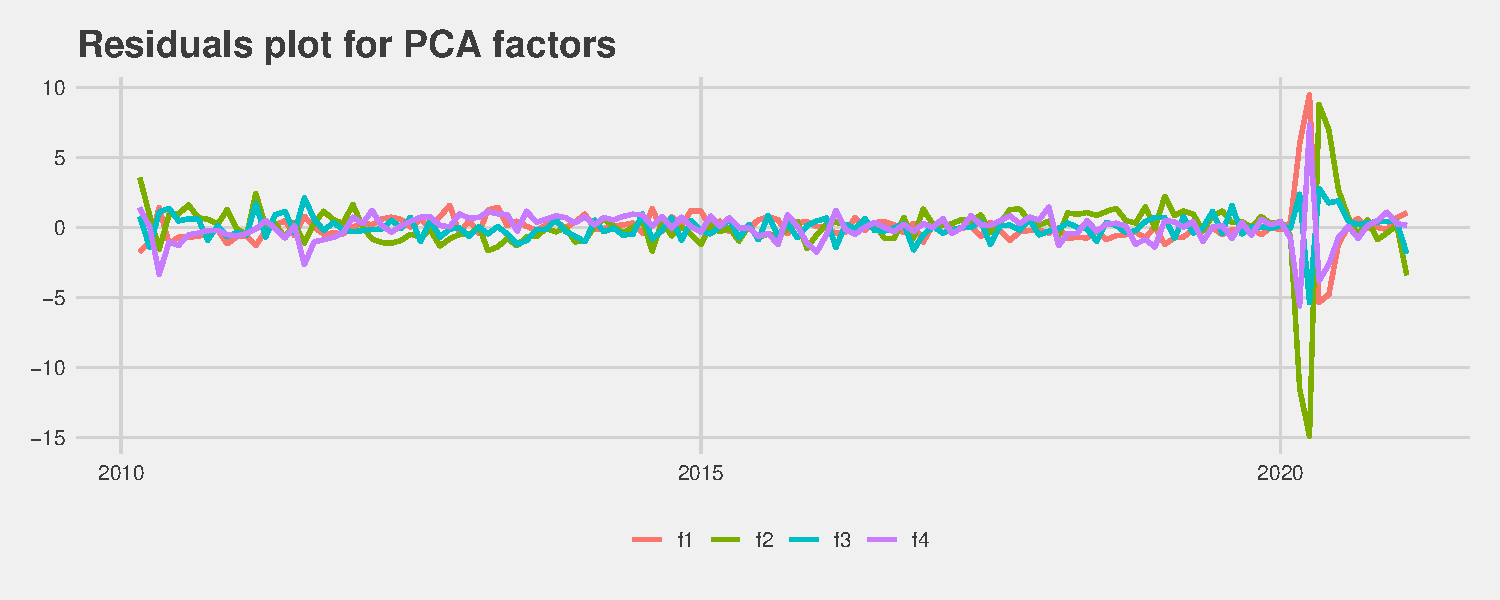
\includegraphics[width=5in,height=2in]{D:/Onedrive/__Projects/econforecasting/model-outputs/latex-figures/unnamed-chunk-13-1} 

}




{\centering 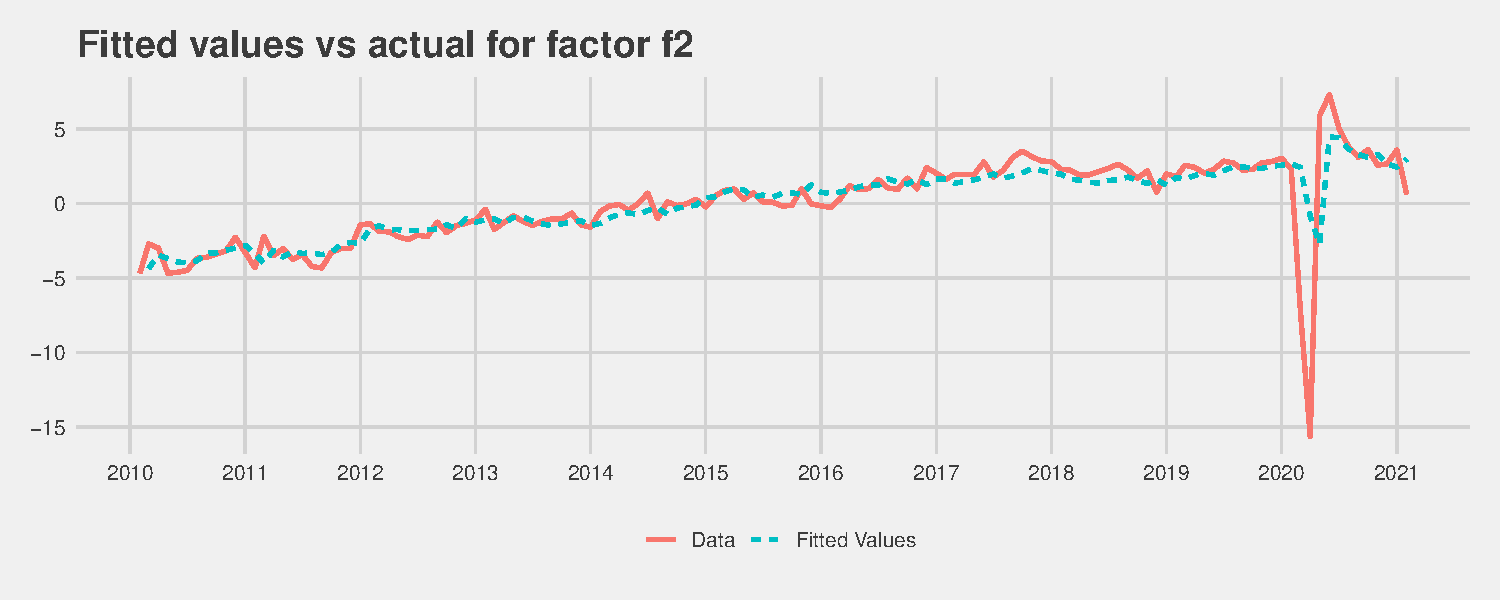
\includegraphics[width=5in,height=2in]{D:/Onedrive/__Projects/econforecasting/model-outputs/latex-figures/unnamed-chunk-13-2} 

}





\begin{figure}[H]

{\centering 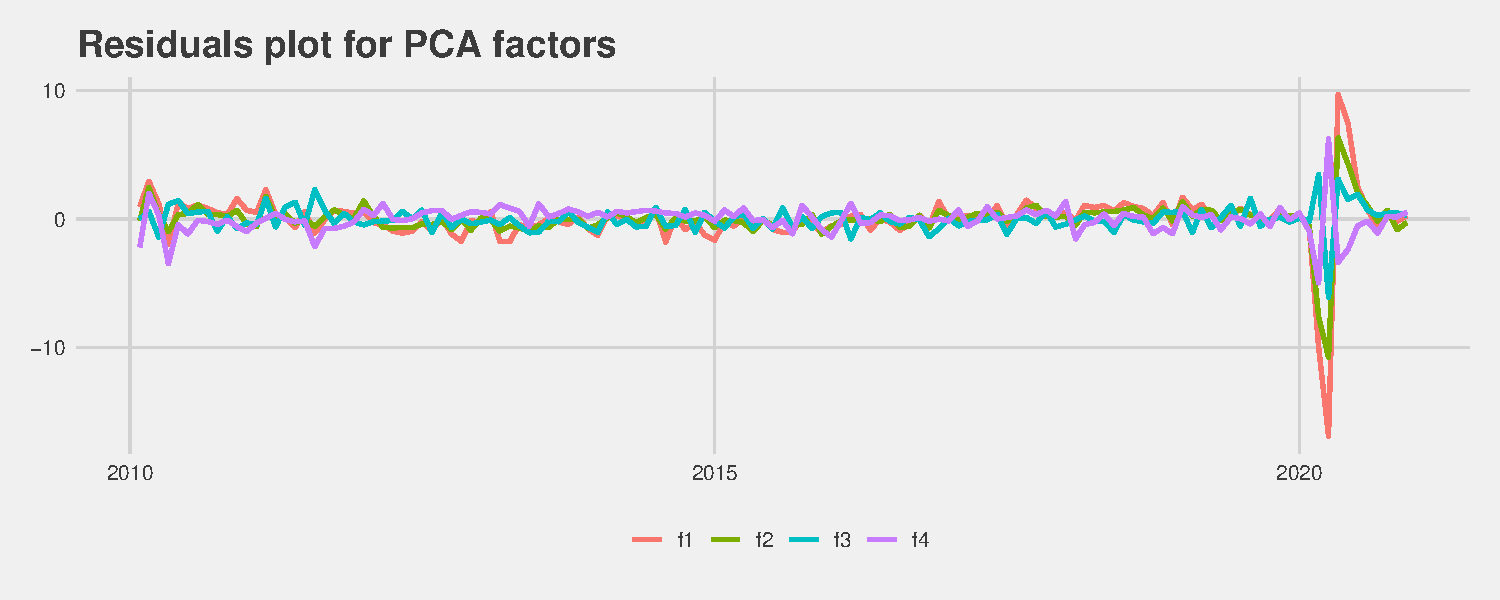
\includegraphics[width=5in,height=2in]{D:/Onedrive/__Projects/econforecasting/model-outputs/latex-figures/unnamed-chunk-14-1} 

}

\caption[Factor VAR Residuals]{Factor VAR Residuals}\label{fig:unnamed-chunk-14}
\end{figure}



Additionally, we expect residuals of the nowcast. Goodness-of-fit statistics are shown below.
% latex table generated in R 4.0.4 by xtable 1.8-4 package
% Sun May 09 00:54:33 2021
\begin{table}[H]
\centering
\begingroup\footnotesize
\begin{tabular}{lrr}
  \hline
varname & MAE & MSE \\ 
  \hline
f1 & 0.79659831 & 3.85314533 \\ 
  f2 & 0.78768494 & 3.40039606 \\ 
   \hline
\end{tabular}
\endgroup
\caption{DFM Goodness of Fit} 
\end{table}




\subsection{Dynamic Factor Models}
Now let us consider again the monthly leading economic variables which were include in the principal components analysis. We will model these as dynamic factor models (DFMs), i.e. - they are regressed on the factor variables derived from earlier. As before, let $x^i_t$ refer to the time $t$ value for monthly variable $x^i$, where $i = 1, \dots, N$.

The factor models take the following form:
\begin{align*}
\underbrace{\begin{bmatrix}
	x^1_t\\
	x^2_t\\
	\vdots \\
	x^N_t
\end{bmatrix}}_{y_t}
=
A
\underbrace{\begin{bmatrix}
	f^1_{t}\\
	f^2_{t}\\
	\vdots \\
	f^R_{t}
\end{bmatrix}}_{z_t}
+
D 
+
\underbrace{\begin{bmatrix}
	w^1_t\\
	w^2_t\\
	\vdots\\
	w^N_t
\end{bmatrix}}_{w_t},\\
\text{where $y_t$ is the $N \times 1$ vector of monthly variables at time $t$,}\\
\text{$A$ is the $N \times R$ coefficient matrix,}\\
\text{$z_t$ is the $R \times 1$ vector of factors at time $t$,}\\
\text{$D$ is the $N \times 1$ constant matrix,}\\
\text{and $w_t$ is the $N \times 1$ vector of errors at time $t$.}\\
\end{align*}
We wish to estimate the coefficient matrices $A$ and $D$. As before, we can do this by estimating this as an OLS equation, writing the data matrices as follows

\begin{equation}
\underbrace{\begin{bmatrix}
x^1_{2} & x^2_{2} & \dots & x^N_{2}\\
x^1_{3} & x^2_{3} & \dots & x^N_{3}\\
\vdots & \vdots & \vdots & \vdots \\
x^1_{T} & x^2_{T} & \dots & x^N_{T}\\
\end{bmatrix}}_{\Phi}
=
\underbrace{\begin{bmatrix}
1 & f^1_{2} & f^2_{2} & \dots & f^R_{2}\\
1 & f^1_{3} & f^2_{3} & \dots & f^R_{3}\\
\vdots & \vdots & \vdots & \vdots & \vdots \\
1 & f^1_{T} & f^2_{T} & \dots & f^R_{T}\\
\end{bmatrix}}_{\Omega}
\begin{bmatrix}
D'\\
A'
\end{bmatrix}
 +
\underbrace{\begin{bmatrix}
w^1_2 & w^2_2 & \dots & w^R_2\\
w^1_3 & w^2_3 & \dots & w^R_3\\
\vdots\\
w^1_T & w^2_T & \dots & w^R_T\\
\end{bmatrix}}_{W}
\end{equation}

However, estimation of $A$ and $D$ with the standard OLS estimator is likely to lead to significant overfitting, particularly if the matrix of $f$ factors is particularly high-dimensional. We will instead use an elastic net process to regularize covariate selection (Zou and Hastie 2005). Hyperparameters of the elastic net are chosen through a cross-validated MAE-minimization process.
% As before we can estimate $A$ and $D$ with the standard OLS estimator.
% \begin{align*}
% \begin{bmatrix}
% 	\widehat{A}\\
% 	\widehat{D}
% \end{bmatrix} =
% (\Omega' \Omega)^{-1} (\Omega'\Phi)
% \end{align*}

Estimated coefficients for $\widehat{A}$ and $\widehat{D}$ are below.
% latex table generated in R 4.0.4 by xtable 1.8-4 package
% Sun May 09 00:54:33 2021
\begin{table}[H]
\centering
\begingroup\footnotesize
\begin{tabular}{lrrr}
  \hline
name & constant & f1 & f2 \\ 
  \hline
mpce & 0.00 & 0.00 & 0.00 \\ 
  pid & 0.00 & -0.00 & -0.00 \\ 
  hpi & 0.00 & -0.00 & 0.00 \\ 
  houst & 0.01 & 0.01 & 0.01 \\ 
  hsold & 0.01 & 0.00 & 0.01 \\ 
  hpermits & 0.01 & 0.01 & 0.01 \\ 
  mnodg & 0.00 & 0.01 & 0.01 \\ 
  cu & 0.00 & 0.00 & 0.00 \\ 
  cons & 0.00 & 0.00 & 0.00 \\ 
  ffr & 0.59 & -0.06 & 0.12 \\ 
  t10y & 2.24 & 0.14 & -0.06 \\ 
  t01y & 2.24 & 0.14 & -0.06 \\ 
  vsales & 16.02 & -0.17 & 0.55 \\ 
  ue & -0.00 & -0.03 & -0.02 \\ 
  joltshires & 5108.83 & -93.54 & 210.95 \\ 
  wei & 1.57 & 0.48 & -0.15 \\ 
  spy & 0.01 & 0.00 & 0.00 \\ 
  vix & 18.04 & -0.77 & -1.05 \\ 
  oil & 69.13 & 5.59 & -3.51 \\ 
  loansre & 0.00 & -0.00 & 0.00 \\ 
  loanscc & 0.01 & 0.00 & -0.00 \\ 
  stlfsi & -0.26 & -0.09 & -0.09 \\ 
  usd & 103.99 & -2.64 & 2.37 \\ 
  uemean & 29.62 & 1.72 & -1.34 \\ 
  advsales & 0.00 & 0.00 & 0.00 \\ 
  kclfi & -0.46 & -0.15 & 0.28 \\ 
  csent & 99.78 & -0.21 & 0.31 \\ 
  ipi & 0.00 & 0.00 & 0.00 \\ 
  pcepi & 0.00 & 0.00 & 0.00 \\ 
  snyfed & 6.14 & 2.68 & 1.52 \\ 
  stxfed & 2.52 & 2.77 & 2.54 \\ 
  sphfed & 21.28 & -0.30 & 1.92 \\ 
  cfnai & -0.07 & 0.41 & 0.39 \\ 
  baa & 4.83 & 0.14 & -0.15 \\ 
  lfpr & 63.11 & 0.20 & -0.14 \\ 
   \hline
\end{tabular}
\endgroup
\caption{Estimated DFM Coefficients} 
\end{table}


We perform a qualitative check of the in-sample fit, as well as a quantitative review of the goodness-of-fit. The graphs of the fitted plots are located in the appendix.
% latex table generated in R 4.0.4 by xtable 1.8-4 package
% Sun May 09 00:54:33 2021
\begin{table}[H]
\centering
\begingroup\footnotesize
\begin{tabular}{lrr}
  \hline
varname & MAE & MSE \\ 
  \hline
advsales & 0.00836104 & 0.00026492 \\ 
  baa & 0.30390371 & 0.15041370 \\ 
  cfnai & 0.48158019 & 0.47205585 \\ 
  cons & 0.00861200 & 0.00011795 \\ 
  csent & 0.68834117 & 0.93922367 \\ 
  cu & 0.00497833 & 0.00004933 \\ 
  ffr & 0.49116800 & 0.40321928 \\ 
  houst & 0.06828199 & 0.00690219 \\ 
  hpermits & 0.04087848 & 0.00260308 \\ 
  hpi & 0.00281562 & 0.00001413 \\ 
  hsold & 0.06064520 & 0.00645225 \\ 
  ipi & 0.00483713 & 0.00004636 \\ 
  joltshires & 179.06485405 & 72773.12863989 \\ 
  kclfi & 0.36826681 & 0.31153245 \\ 
  lfpr & 0.33725031 & 0.19095050 \\ 
  loanscc & 0.01518229 & 0.00225512 \\ 
  loansre & 0.00216736 & 0.00000855 \\ 
  mnodg & 0.02991167 & 0.00183419 \\ 
  mpce & 0.00500767 & 0.00006665 \\ 
  oil & 11.12140903 & 173.71219846 \\ 
  pcepi & 0.00099890 & 0.00000162 \\ 
  pid & 0.00742623 & 0.00028176 \\ 
  snyfed & 7.59956351 & 103.97124248 \\ 
  sphfed & 6.64275871 & 65.09954734 \\ 
  spy & 0.02188327 & 0.00103215 \\ 
  stlfsi & 0.28650872 & 0.16443336 \\ 
  stxfed & 10.61640804 & 188.24390636 \\ 
  t01y & 0.42577771 & 0.27606945 \\ 
  t10y & 0.42577771 & 0.27606945 \\ 
  ue & 0.03701340 & 0.00282496 \\ 
  uemean & 2.91457980 & 13.34413116 \\ 
  usd & 3.34612266 & 16.84548859 \\ 
  vix & 4.26198721 & 33.48422920 \\ 
  vsales & 0.94146682 & 1.86923762 \\ 
  wei & 1.20791709 & 3.65727335 \\ 
   \hline
\end{tabular}
\endgroup
\caption{DFM Goodness of Fit} 
\end{table}





\subsection{State-Space Setup}
Now, combining our equations for the DFM and the VAR, we have the below system.
\begin{align*}
z_t = B z_{t-1} + Cx + v_t\\
y_t = A z_t + w_t
\end{align*}

This system is now fully specified and in state-space form. The first equation is our state (or transition) equation. The second equation is our measurement equation. 

We use our estimated values $B$, $C$, $A$, and $D$ calculated in our previous two sections. To run the Kalman Filter, we will want to create the actual data matrices for $z_t$ and $y_t$. $z_t$ can be constructed as before, using data for factors from time 1 through $T$. However, unlike in the previous two sections, we will want to create $y_t$ matrices not for just time periods 1 through $T$, but now for time periods $1$ through $\tau$. Elements in $y_t$ may be set to any value for missing observations; the process of Kalmam filtration will render this choice irrelevant.

Specifically, we construct the matrices below.
\begin{align*}
z_t
=
\begin{bmatrix}
	f^1_{t}\\
	f^2_{t}\\
	\vdots \\
	f^R_{t}
\end{bmatrix}, \forall t \in 1, \dots, T\\
y_t
=
\begin{bmatrix}
	\text{$x^1_{t}$ if available, otherwise 0}\\
	\text{$x^2_{t}$ if available, otherwise 0}\\
	\vdots \\
	\text{$x^N_{t}$ if available, otherwise 0}\\
\end{bmatrix}, \forall t \in 1, \dots, \tau
\end{align*}

For Kalman filtration, we also require an assumed distribution on $v_t$ and $w_t$. We assume that $v_t$ is distributed normally with mean 0 and constant diagonal covariance matrix denoted $Q$, with diagonal entries calculated by taking the average squared values of the residuals of the VAR.

We also assume $w_t$ is distributed normally with mean $0$. However, we no longer specify the covariance matrix as constant, but as the time-dependent matrices $R_t$. For $t \in 1, \dots, T+1$, we let $R_t$ be a diagonal covariance matrix with diagonal entries calcualted by taking the average squared values of the residuals of the DFM. For $t \in T+1, \dots, \tau$, we let the diagonal elements of $R_t$ be equal to infinity if the corresponding element of $y_t$ is missing for that time period; and equal to the average squared value of the residual if otherwise.
\begin{align*}
	v_t \sim \mathcal{N}(0, Q)\\
	w_t \sim \mathcal{N}(0, R_t)
\end{align*}

\subsection{Kalman Filtration}
Now that our state-space model is fully specified, we can begin the Kalman filter recursions.
\begin{align*}
	z_t = B z_{t-1} + Cx + v_t\\
	y_t = A z_t + Dx + w_t\\
	v_t \sim \mathcal{N}(0, Q)\\
	w_t \sim \mathcal{N}(0, R_t)
\end{align*}

To solve this programmatically, we will need the previously estimated matrices $A$, $B$, $C$, and $D$; the matrices $z_t$ from 1 through $T$; the matrices $y_t$ from 1 through $\tau$; the covariance matrix $Q$; and finally, the covariance matrices $R_t$ from 1 through $\tau$.

We initialize the Kalman filter with the following standard assumptions. 
\begin{align*}
	\vv{z}_{0|0} = 0\\
	\vv{CovZ} = 0
\end{align*}

Now for $t = 1, \dots, \tau$, we iterate through the Kalman filter recursions and iteratively calculate the values below.
\begin{align*}
	\vv{z}_{t|t-1} &= B \vv{z}_{t-1|t-1} + C\\
	\vv{CovZ}_{t|t-1} &= B \vv{CovZ}_{t-1|t-1} + Q\\
	\vv{y}_{t|t-1} &= A \vv{z}_{t|t-1} + D\\
	\vv{CovY}_{t|t-1} &= A \vv{CovZ}_{t|t-1} A' + R_t\\
	P_t &= \vv{CovZ}_{t|t-1} A' \vv{CovY}^{-1}_{t|t-1}\\
	\vv{z}_{t|t} &= \vv{z}_{t|t-1} + P_t (\vv{y}_t - \vv{y}_{t|t-1})\\
	\vv{CovZ}_{t|t} &= \vv{CovZ}_{t|t-1} - P_t (\vv{CovY}_{t|t-1}) P'_t
\end{align*}
Note that the during recursions $T + 1, \dots \tau$, the infinite values in the $R_t$ matrix will cause infinite values in the $\vv{CovY}_{t|t-1}$ matrix. This may prevent standard computational methods from computing the inverse of the matrix needed in the step for calculation of $\vv{CovZ}_{t|t}$. Alternative methods, such as a Cholesky decomposition before inversion, are used to subvert this problem.

The Kalman filter allows us to recover all the time $t$ conditional state matrices $z_{t|t}$ that have been adjusted for information from the monthly datasets. However, of more interest to us is the value of the state matrices when conditioned on all data available at time $\tau$, $z_{t|\tau}$. This can be recovered by using the Kalman smoother.

Recursively iterating over $t = \tau - 1, \dots, 1$, we calculate the following values. 
\begin{align*}
	S_{t} &= \vv{CovZ}_{t|t} B' \vv{CovZ}^{-1}_{t + 1|t}\\
	\vv{z}_{t|\tau} &= \vv{z}_{t|t} + S_t (\vv{z}_{t+1|\tau} - \vv{z}_{t + 1|t})\\
	\vv{CovZ}_{t|\tau} &= \vv{CovZ}_{t|t} - S_t(\vv{CovZ}_{t + 1|t} - \vv{CovZ}_{t + 1|\tau})S'_t
\end{align*}
These values $\vv{z}_{t|\tau}$ will serve as our estimates of the state variables (i.e., the PCA factors) from time 1 through $\tau$.

Finally, we want to forecast the the state vector $z_{t|\tau}$ for $t = \tau + 1, \dots, T^*$. This can be done through the typical Kalman filter forecasting step.

Recursively iterating over $t = \tau + 1, \dots, T^*$, we calculate the following values.
\begin{align*}
	\vv{z}_{t|\tau} &= B \vv{z}_{t-1|\tau} + C\\
	\vv{CovZ}_{t|\tau} &= B \vv{CovZ}_{t-1|\tau} B'+ Q\\
	\vv{y}_{t|\tau} &= A \vv{z}_{t|\tau} + D\\
	\vv{CovY}_{t|\tau} &= A \vv{CovZ}_{t|\tau} A' + R_0
\end{align*}
Combining the calculations for $\vv{z}_{t|\tau}$ with the ones derived from the Kalman smoother, we will now be able to obtain the full time series for the factors from time 1 through time $T^*$.



{\centering 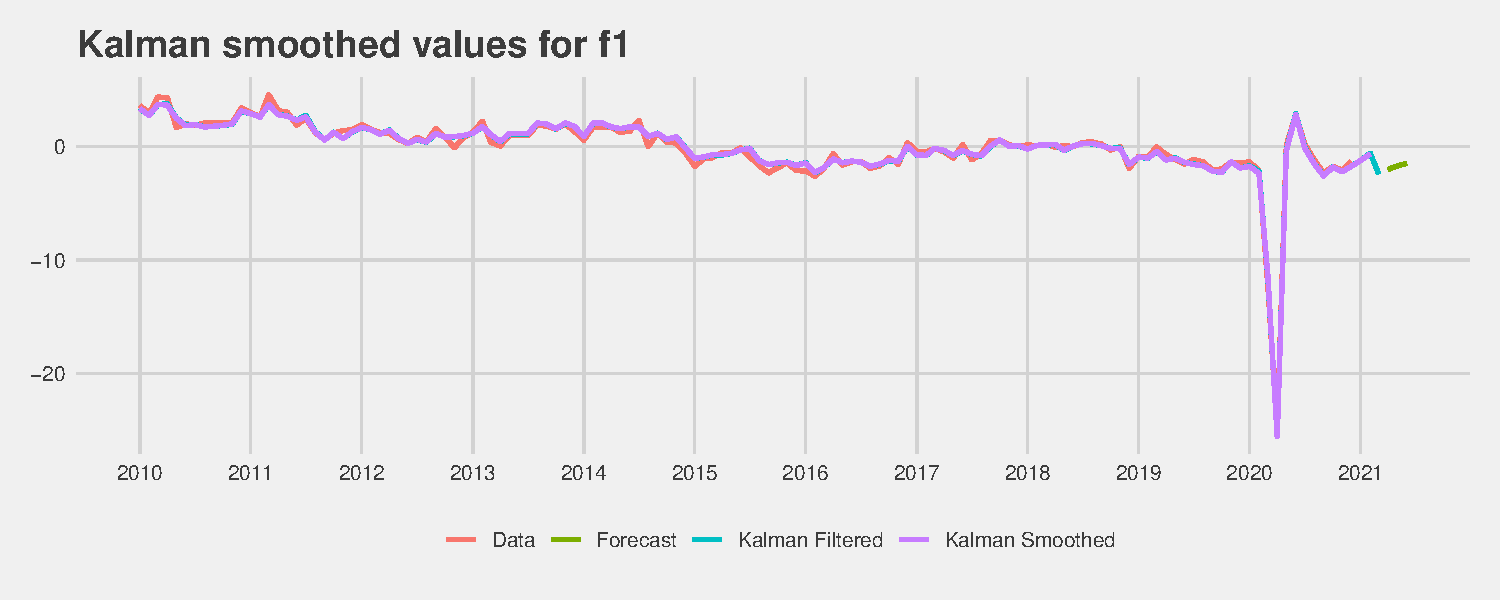
\includegraphics[width=5in,height=2in]{D:/Onedrive/__Projects/econforecasting/model-outputs/latex-figures/unnamed-chunk-18-1} 

}




{\centering 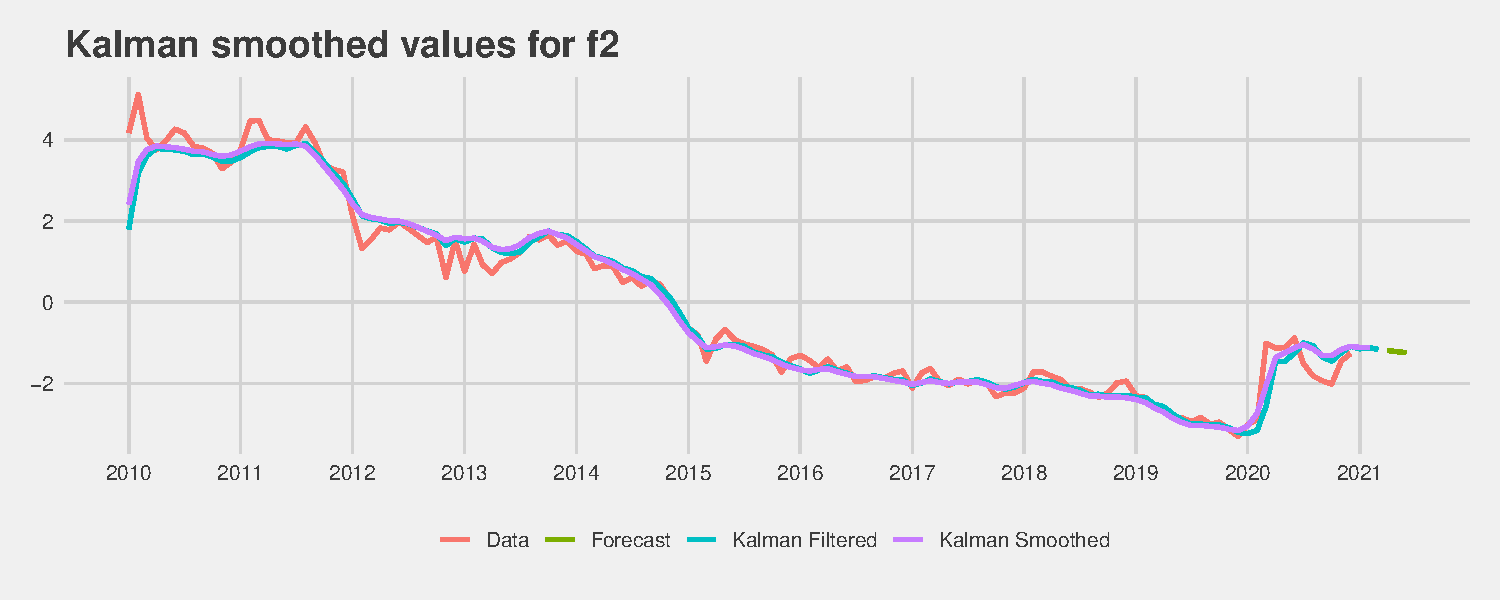
\includegraphics[width=5in,height=2in]{D:/Onedrive/__Projects/econforecasting/model-outputs/latex-figures/unnamed-chunk-18-2} 

}




% \subsection{Nowcasting Monthly Covariates}
% Now that we have our Kalman-smoothed factors from time $1$ through time $T^*$, we will be able to use these as covariates to model any monthly time series that we have. 

\subsection{Nowcast Step}
Now that we have our Kalman-smoothed and forecasted factors from time $1$ through time $T^*$, we will be able to use these as covariates to model any monthly time series that we have.

We begin by aggregating these monthly factors into quarterly data by taking a simple monthly average for each factor over each quarter.

In this section, we will use these now-quarterly factors to forecast our quarterly subcomponents of GDP. As discussed in the data import section, these have been transformed for stationarity, typically by taking a log-difference.
% latex table generated in R 4.0.4 by xtable 1.8-4 package
% Sun May 09 00:54:33 2021
\begin{table}[H]
\centering
\begingroup\scriptsize
\begin{tabular}{l}
  \hline
Variable \\ 
  \hline
Consumption: Goods: Durable: Motor Vehicles \& Parts \\ 
  Consumption: Goods: Durable: Furnishings \& Durable Household Equipment \\ 
  Consumption: Goods: Durable: Recreational Goods \& Services \\ 
  Consumption: Goods: Durable: Other Durable Goods \\ 
  Consumption: Goods: Nondurable Goods: Food \& Beverages for Off-Premises Use \\ 
  Consumption: Goods: Nondurable Goods: Clothing \\ 
  Consumption: Goods: Nondurable Goods: Gasoline \& Energy Goods \\ 
  Consumption: Goods: Nondurable Goods: Other Nondurable Goods \\ 
  Consumption: Services: Housing \& Utilities \\ 
  Consumption: Services: Health Care \\ 
  Consumption: Services: Transportation \\ 
  Consumption: Services: Recreation \\ 
  Consumption: Services: Food Services \& Accomodations \\ 
  Consumption: Services: Financial Services \\ 
  Consumption: Services: Other Services \\ 
  Consumption: Services: Nonprofit Services \\ 
  Gross Private Domestic Investment: Nonresidential Investment: Structures \\ 
  Gross Private Domestic Investment: Nonresidential Investment: Equipment \\ 
  Gross Private Domestic Investment: Nonresidential Investment: Intellectual Property \\ 
  Gross Private Domestic Investment: Residential Investment \\ 
  Gross Private Domestic Investment: Change in Private Inventories \\ 
  Exports: Exported Goods \\ 
  Exports: Exported Services \\ 
  Imports: Imported Goods \\ 
  Imports: Imported Services \\ 
  Government Spending: Federal \\ 
  Government Spending: State \& Local \\ 
   \hline
\end{tabular}
\endgroup
\caption{Quarterly Data Covariates} 
\end{table}

We will notate each of these gdp subcomponents as $y^i$ and $M$ as the total number of covariates, so that $i = 1, \dots, M$.

Note that many higher-level components of GDP (including GDP itself) are \textit{not} forecasted directly in this step; these will be forecasted later by aggregating their subcomponents.

Now we will specify that these GDP subcomponents follow a DFM-AR(1) model; i.e., they will be functions of the monthly-aggregated factors as well as the first lag of themselves.
\begin{align*}
	y^i_t
	=
	\beta
	\begin{bmatrix}
	1 \\
	y^i_{t-1}\\
	f^1_t \\
	\vdots\\
	f^R_t
	\end{bmatrix}
	+
	e_t
\end{align*}
The $\beta$ coefficients can be estimated with a typical OLS process, where the training data is constituted of the $y^i_t$ quarterly covariates, the lagged quarterly covariates $y^i_{t-1}$, and the quarterly-aggregated factor variables. The data is cut off at the date for which the any data on the quarterly covariates are missing.

After estimation, we then use the same model to forecast forward the $y^i_t$ quarterly, up through time $\tau$. 
The forecasted results are as follows.
% latex table generated in R 4.0.4 by xtable 1.8-4 package
% Sun May 09 00:54:33 2021
\begin{table}[H]
\centering
\begingroup\scriptsize
\begin{tabular}{lrrr}
  \hline
Variable & 2021Q1 & 2021Q2 & 2021Q3 \\ 
  \hline
Consumption: Goods: Durable: Motor Vehicles \& Parts &  & 0.01 & 0.01 \\ 
  Consumption: Goods: Durable: Furnishings \& Durable Household Equipment &  & 0.04 & 0.01 \\ 
  Consumption: Goods: Durable: Recreational Goods \& Services &  & 0.03 & 0.03 \\ 
  Consumption: Goods: Durable: Other Durable Goods &  & 0.01 & 0.01 \\ 
  Consumption: Goods: Nondurable Goods: Food \& Beverages for Off-Premises Use &  & -0.01 & 0.02 \\ 
  Consumption: Goods: Nondurable Goods: Clothing &  & 0.15 & -0.04 \\ 
  Consumption: Goods: Nondurable Goods: Gasoline \& Energy Goods &  & -0.00 & -0.00 \\ 
  Consumption: Goods: Nondurable Goods: Other Nondurable Goods &  & 0.01 & 0.01 \\ 
  Consumption: Services: Housing \& Utilities &  & 0.00 & 0.00 \\ 
  Consumption: Services: Health Care &  & 0.01 & 0.01 \\ 
  Consumption: Services: Transportation &  & 0.22 & -0.05 \\ 
  Consumption: Services: Recreation &  & -0.00 & -0.00 \\ 
  Consumption: Services: Food Services \& Accomodations &  & 0.00 & 0.00 \\ 
  Consumption: Services: Financial Services &  & 0.01 & 0.00 \\ 
  Consumption: Services: Other Services &  & 0.00 & 0.00 \\ 
  Consumption: Services: Nonprofit Services &  & -0.15 & 0.03 \\ 
  Gross Private Domestic Investment: Nonresidential Investment: Structures &  & 0.01 & -0.00 \\ 
  Gross Private Domestic Investment: Nonresidential Investment: Equipment &  & 0.10 & 0.01 \\ 
  Gross Private Domestic Investment: Nonresidential Investment: Intellectual Property &  & 0.04 & 0.01 \\ 
  Gross Private Domestic Investment: Residential Investment &  & 0.01 & 0.01 \\ 
  Gross Private Domestic Investment: Change in Private Inventories &  & 123.85 & 72.26 \\ 
  Exports: Exported Goods &  & 0.15 & -0.03 \\ 
  Exports: Exported Services &  & 0.10 & 0.02 \\ 
  Imports: Imported Goods &  & 0.01 & 0.01 \\ 
  Imports: Imported Services &  & -0.00 & -0.00 \\ 
  Government Spending: Federal &  & -0.00 & 0.00 \\ 
  Government Spending: State \& Local &  & 0.01 & 0.00 \\ 
   \hline
\end{tabular}
\endgroup
\caption{DFM-AR(1) Forecasted GDP Subcomponents} 
\end{table}


We can then backtransform the data so that the units are in base values. After backtransformation, we are ready to aggregate these up to higher-level GDP components. In particular, we calculate the variables below.
% latex table generated in R 4.0.4 by xtable 1.8-4 package
% Sun May 09 00:54:33 2021
\begin{table}[H]
\centering
\begingroup\scriptsize
\begin{tabular}{l}
  \hline
Variable \\ 
  \hline
GDP \\ 
  Consumption \\ 
  Consumption: Goods \\ 
  Consumption: Goods: Durable \\ 
  Consumption: Goods: Nondurable Goods \\ 
  Consumption: Services \\ 
  Gross Private Domestic Investment \\ 
  Gross Private Domestic Investment: Nonresidential Investment \\ 
  Net Exports \\ 
  Exports \\ 
  Imports \\ 
  Government Spending \\ 
   \hline
\end{tabular}
\endgroup
\caption{Summable Quarterly Data Covariates} 
\end{table}

These are calculated using the standard GDP aggregation equations, e.g., net exports = exports - imports, and so on.
Finally, we convert these into annualized percentage change, as this is the standard format in which GDP subcomponents are reported in. The results are reported in the next section.

We also use a similar DFM-AR(1) specification to forecast out other economic variables of interest, with results reported in the next section.


\section{Results}
Our final nowcasts of GDP and its subcomponents are below. All units are reported in terms of annualized percentage change (seasonally adjusted) except for change in private inventories and net exports, which are reported in terms of billions of real 2012 dollars.
% latex table generated in R 4.0.4 by xtable 1.8-4 package
% Sun May 09 00:54:34 2021
\begin{table}[H]
\centering
\begingroup\fontsize{10pt}{12pt}\selectfont
\begin{tabular}{lrrr}
  \hline
Variable & 2021Q1 & 2021Q2 & 2021Q3 \\ 
  \hline
\hspace{0mm} \textbf{GDP} &  & 23.31 & -0.24 \\ 
  \hspace{0mm} \textbf{Consumption} &  & 12.59 & 1.96 \\ 
  \hspace{8mm}  Goods &  & 13.15 & 3.91 \\ 
  \hspace{16mm}  Durable &  & 17.46 & 7.35 \\ 
  \hspace{24mm}  Motor Vehicles \& Parts &  & 5.53 & 5.53 \\ 
  \hspace{24mm}  Furnishings \& Durable Household Equipment &  & 16.63 & 4.93 \\ 
  \hspace{24mm}  Recreational Goods \& Services &  & 10.89 & 10.89 \\ 
  \hspace{24mm}  Other Durable Goods &  & 6.11 & 6.11 \\ 
  \hspace{16mm}  Nondurable Goods &  & 4.69 & 1.55 \\ 
  \hspace{24mm}  Food \& Beverages for Off-Premises Use &  & -5.10 & 7.43 \\ 
  \hspace{24mm}  Clothing &  & 85.43 & -14.07 \\ 
  \hspace{24mm}  Gasoline \& Energy Goods &  & -0.54 & -1.12 \\ 
  \hspace{24mm}  Other Nondurable Goods &  & 5.52 & 4.32 \\ 
  \hspace{8mm}  Services &  & 2.92 & 0.65 \\ 
  \hspace{16mm}  Housing \& Utilities &  & 1.24 & 1.24 \\ 
  \hspace{16mm}  Health Care &  & 2.06 & 2.06 \\ 
  \hspace{16mm}  Transportation &  & 145.76 & -17.35 \\ 
  \hspace{16mm}  Recreation &  & -1.51 & -1.51 \\ 
  \hspace{16mm}  Food Services \& Accomodations &  & 0.51 & 0.51 \\ 
  \hspace{16mm}  Financial Services &  & 4.65 & 1.83 \\ 
  \hspace{16mm}  Other Services &  & 0.91 & 0.91 \\ 
  \hspace{16mm}  Nonprofit Services &  & -44.06 & 12.99 \\ 
  \hspace{0mm} \textbf{Gross Private Domestic Investment} &  & 49.67 & -1.95 \\ 
  \hspace{8mm}  Nonresidential Investment &  & 33.29 & 3.07 \\ 
  \hspace{16mm}  Structures &  & 4.16 & -1.46 \\ 
  \hspace{16mm}  Equipment &  & 48.04 & 2.65 \\ 
  \hspace{16mm}  Intellectual Property &  & 15.44 & 5.65 \\ 
  \hspace{8mm}  Residential Investment &  & 5.46 & 5.46 \\ 
  \hspace{8mm}  Change in Private Inventories &  & 123.85 & 72.26 \\ 
  \hspace{0mm} \textbf{Net Exports} &  & -863.89 & -935.79 \\ 
  \hspace{0mm} \textbf{Exports} &  & 85.09 & -6.54 \\ 
  \hspace{8mm}  Exported Goods &  & 82.98 & -10.76 \\ 
  \hspace{8mm}  Exported Services &  & 51.51 & 7.36 \\ 
  \hspace{0mm} \textbf{Imports} &  & 7.94 & 3.16 \\ 
  \hspace{8mm}  Imported Goods &  & 3.61 & 3.61 \\ 
  \hspace{8mm}  Imported Services &  & -0.10 & -0.10 \\ 
  \hspace{0mm} \textbf{Government Spending} &  & 0.67 & 1.41 \\ 
  \hspace{8mm}  Federal &  & -1.94 & 1.52 \\ 
  \hspace{8mm}  State \& Local &  & 2.05 & 1.33 \\ 
   \hline 
 \textit{apchg} = annualized \% change 
\end{tabular}
\endgroup
\caption{Nowcasts for GDP and Subcomponents (Annualized Percent Change)} 
\end{table}


We also report nowcasts of other variables of interest, including other quarterly variables, as well as all monthly variables used in this process. Note that because these variables are ragged-edge in nature, there may be "blank" columns. These columns simply indicate that historical data already exists for those columns. Only nowcasts produced by the model are reported.
% latex table generated in R 4.0.4 by xtable 1.8-4 package
% Sun May 09 00:54:34 2021
\begin{table}[H]
\centering
\begingroup\fontsize{11pt}{13pt}\selectfont
\begin{tabular}{lrrr}
  \hline
Variable & 2021Q1 & 2021Q2 & 2021Q3 \\ 
  \hline
Delinquency Rate on Residential Mortgages & 2.58 & 2.33 & 2.31 \\ 
  Delinquency Rate on Credit Cards & 2.16 & 2.20 & 2.23 \\ 
  Delinquency Rate on Commercial $\backslash$\& Industrial Loans & 1.28 & 1.19 & 1.19 \\ 
   \hline
\end{tabular}
\endgroup
\caption{Nowcasts for Other Quarterly Variables} 
\end{table}

% latex table generated in R 4.0.4 by xtable 1.8-4 package
% Sun May 09 00:54:34 2021
\begin{table}[H]
\centering
\begingroup\fontsize{10pt}{12pt}\selectfont
\begin{tabular}{lrrrrrrrrrrrrrrrrrrrrrrrrrrrrrrrrrrrrrrrrrrrrrrrrrrrrrrrrrrrrrrrrrrrrrrrrrrrrrrrrrrrrrrrrrrrrrrrrrrrrrrrrrrrrrrrrrrrrrrrrrrrrrrrrrrrrrrrrrrrr}
  \hline
Variable & 2010M2 & 2010M3 & 2010M4 & 2010M5 & 2010M6 & 2010M7 & 2010M8 & 2010M9 & 2010M10 & 2010M11 & 2010M12 & 2011M1 & 2011M2 & 2011M3 & 2011M4 & 2011M5 & 2011M6 & 2011M7 & 2011M8 & 2011M9 & 2011M10 & 2011M11 & 2011M12 & 2012M1 & 2012M2 & 2012M3 & 2012M4 & 2012M5 & 2012M6 & 2012M7 & 2012M8 & 2012M9 & 2012M10 & 2012M11 & 2012M12 & 2013M1 & 2013M2 & 2013M3 & 2013M4 & 2013M5 & 2013M6 & 2013M7 & 2013M8 & 2013M9 & 2013M10 & 2013M11 & 2013M12 & 2014M1 & 2014M2 & 2014M3 & 2014M4 & 2014M5 & 2014M6 & 2014M7 & 2014M8 & 2014M9 & 2014M10 & 2014M11 & 2014M12 & 2015M1 & 2015M2 & 2015M3 & 2015M4 & 2015M5 & 2015M6 & 2015M7 & 2015M8 & 2015M9 & 2015M10 & 2015M11 & 2015M12 & 2016M1 & 2016M2 & 2016M3 & 2016M4 & 2016M5 & 2016M6 & 2016M7 & 2016M8 & 2016M9 & 2016M10 & 2016M11 & 2016M12 & 2017M1 & 2017M2 & 2017M3 & 2017M4 & 2017M5 & 2017M6 & 2017M7 & 2017M8 & 2017M9 & 2017M10 & 2017M11 & 2017M12 & 2018M1 & 2018M2 & 2018M3 & 2018M4 & 2018M5 & 2018M6 & 2018M7 & 2018M8 & 2018M9 & 2018M10 & 2018M11 & 2018M12 & 2019M1 & 2019M2 & 2019M3 & 2019M4 & 2019M5 & 2019M6 & 2019M7 & 2019M8 & 2019M9 & 2019M10 & 2019M11 & 2019M12 & 2020M1 & 2020M2 & 2020M3 & 2020M4 & 2020M5 & 2020M6 & 2020M7 & 2020M8 & 2020M9 & 2020M10 & 2020M11 & 2020M12 & 2021M1 & 2021M2 & 2021M3 & 2021M4 & 2021M5 & 2021M6 & 2021M7 & 2021M8 & 2021M9 \\ 
  \hline
PCE \textit{\footnotesize\textcolor{gray}{(apchg)}} &  &  &  &  &  &  &  &  &  &  &  &  &  &  &  &  &  &  &  &  &  &  &  &  &  &  &  &  &  &  &  &  &  &  &  &  &  &  &  &  &  &  &  &  &  &  &  &  &  &  &  &  &  &  &  &  &  &  &  &  &  &  &  &  &  &  &  &  &  &  &  &  &  &  &  &  &  &  &  &  &  &  &  &  &  &  &  &  &  &  &  &  &  &  &  &  &  &  &  &  &  &  &  &  &  &  &  &  &  &  &  &  &  &  &  &  &  &  &  &  &  &  &  &  &  &  &  &  &  &  &  &  &  &  & 38.21 & 11.11 & 5.98 & 4.17 & 3.52 & 3.29 \\ 
  PCE: Goods \textit{\footnotesize\textcolor{gray}{(apchg)}} &  &  &  &  &  &  &  &  &  &  &  &  &  &  &  &  &  &  &  &  &  &  &  &  &  &  &  &  &  &  &  &  &  &  &  &  &  &  &  &  &  &  &  &  &  &  &  &  &  &  &  &  &  &  &  &  &  &  &  &  &  &  &  &  &  &  &  &  &  &  &  &  &  &  &  &  &  &  &  &  &  &  &  &  &  &  &  &  &  &  &  &  &  &  &  &  &  &  &  &  &  &  &  &  &  &  &  &  &  &  &  &  &  &  &  &  &  &  &  &  &  &  &  &  &  &  &  &  &  &  &  &  &  &  & 41.96 & 14.64 & 9.46 & 7.64 & 6.99 & 6.77 \\ 
  PCE: Goods: Durable Goods \textit{\footnotesize\textcolor{gray}{(apchg)}} &  &  &  &  &  &  &  &  &  &  &  &  &  &  &  &  &  &  &  &  &  &  &  &  &  &  &  &  &  &  &  &  &  &  &  &  &  &  &  &  &  &  &  &  &  &  &  &  &  &  &  &  &  &  &  &  &  &  &  &  &  &  &  &  &  &  &  &  &  &  &  &  &  &  &  &  &  &  &  &  &  &  &  &  &  &  &  &  &  &  &  &  &  &  &  &  &  &  &  &  &  &  &  &  &  &  &  &  &  &  &  &  &  &  &  &  &  &  &  &  &  &  &  &  &  &  &  &  &  &  &  &  &  &  & 63.92 & 22.72 & 15.27 & 12.68 & 11.77 & 11.46 \\ 
  PCE: Goods: Nondurable Goods \textit{\footnotesize\textcolor{gray}{(apchg)}} &  &  &  &  &  &  &  &  &  &  &  &  &  &  &  &  &  &  &  &  &  &  &  &  &  &  &  &  &  &  &  &  &  &  &  &  &  &  &  &  &  &  &  &  &  &  &  &  &  &  &  &  &  &  &  &  &  &  &  &  &  &  &  &  &  &  &  &  &  &  &  &  &  &  &  &  &  &  &  &  &  &  &  &  &  &  &  &  &  &  &  &  &  &  &  &  &  &  &  &  &  &  &  &  &  &  &  &  &  &  &  &  &  &  &  &  &  &  &  &  &  &  &  &  &  &  &  &  &  &  &  &  &  &  & 31.87 & 10.68 & 6.56 & 5.11 & 4.59 & 4.41 \\ 
  PCE: Services \textit{\footnotesize\textcolor{gray}{(apchg)}} &  &  &  &  &  &  &  &  &  &  &  &  &  &  &  &  &  &  &  &  &  &  &  &  &  &  &  &  &  &  &  &  &  &  &  &  &  &  &  &  &  &  &  &  &  &  &  &  &  &  &  &  &  &  &  &  &  &  &  &  &  &  &  &  &  &  &  &  &  &  &  &  &  &  &  &  &  &  &  &  &  &  &  &  &  &  &  &  &  &  &  &  &  &  &  &  &  &  &  &  &  &  &  &  &  &  &  &  &  &  &  &  &  &  &  &  &  &  &  &  &  &  &  &  &  &  &  &  &  &  &  &  &  &  & 36.30 & 9.43 & 4.33 & 2.54 & 1.89 & 1.66 \\ 
  Personal Income \textit{\footnotesize\textcolor{gray}{(apchg)}} &  &  &  &  &  &  &  &  &  &  &  &  &  &  &  &  &  &  &  &  &  &  &  &  &  &  &  &  &  &  &  &  &  &  &  &  &  &  &  &  &  &  &  &  &  &  &  &  &  &  &  &  &  &  &  &  &  &  &  &  &  &  &  &  &  &  &  &  &  &  &  &  &  &  &  &  &  &  &  &  &  &  &  &  &  &  &  &  &  &  &  &  &  &  &  &  &  &  &  &  &  &  &  &  &  &  &  &  &  &  &  &  &  &  &  &  &  &  &  &  &  &  &  &  &  &  &  &  &  &  &  &  &  &  & -8.11 & 1.66 & 3.92 & 4.76 & 5.07 & 5.19 \\ 
  Disposable Personal Income \textit{\footnotesize\textcolor{gray}{(apchg)}} &  &  &  &  &  &  &  &  &  &  &  &  &  &  &  &  &  &  &  &  &  &  &  &  &  &  &  &  &  &  &  &  &  &  &  &  &  &  &  &  &  &  &  &  &  &  &  &  &  &  &  &  &  &  &  &  &  &  &  &  &  &  &  &  &  &  &  &  &  &  &  &  &  &  &  &  &  &  &  &  &  &  &  &  &  &  &  &  &  &  &  &  &  &  &  &  &  &  &  &  &  &  &  &  &  &  &  &  &  &  &  &  &  &  &  &  &  &  &  &  &  &  &  &  &  &  &  &  &  &  &  &  &  &  & -10.70 & 1.15 & 3.94 & 4.97 & 5.36 & 5.50 \\ 
  Personal Outlays \textit{\footnotesize\textcolor{gray}{(apchg)}} &  &  &  &  &  &  &  &  &  &  &  &  &  &  &  &  &  &  &  &  &  &  &  &  &  &  &  &  &  &  &  &  &  &  &  &  &  &  &  &  &  &  &  &  &  &  &  &  &  &  &  &  &  &  &  &  &  &  &  &  &  &  &  &  &  &  &  &  &  &  &  &  &  &  &  &  &  &  &  &  &  &  &  &  &  &  &  &  &  &  &  &  &  &  &  &  &  &  &  &  &  &  &  &  &  &  &  &  &  &  &  &  &  &  &  &  &  &  &  &  &  &  &  &  &  &  &  &  &  &  &  &  &  &  & 41.30 & 12.88 & 7.52 & 5.63 & 4.95 & 4.71 \\ 
  Personal Savings \textit{\footnotesize\textcolor{gray}{(apchg)}} &  &  &  &  &  &  &  &  &  &  &  &  &  &  &  &  &  &  &  &  &  &  &  &  &  &  &  &  &  &  &  &  &  &  &  &  &  &  &  &  &  &  &  &  &  &  &  &  &  &  &  &  &  &  &  &  &  &  &  &  &  &  &  &  &  &  &  &  &  &  &  &  &  &  &  &  &  &  &  &  &  &  &  &  &  &  &  &  &  &  &  &  &  &  &  &  &  &  &  &  &  &  &  &  &  &  &  &  &  &  &  &  &  &  &  &  &  &  &  &  &  &  &  &  &  &  &  &  &  &  &  &  &  &  & -80.21 & -21.43 & 6.01 & 18.27 & 23.10 & 24.93 \\ 
  Personal Savings Rate &  &  &  &  &  &  &  &  &  &  &  &  &  &  &  &  &  &  &  &  &  &  &  &  &  &  &  &  &  &  &  &  &  &  &  &  &  &  &  &  &  &  &  &  &  &  &  &  &  &  &  &  &  &  &  &  &  &  &  &  &  &  &  &  &  &  &  &  &  &  &  &  &  &  &  &  &  &  &  &  &  &  &  &  &  &  &  &  &  &  &  &  &  &  &  &  &  &  &  &  &  &  &  &  &  &  &  &  &  &  &  &  &  &  &  &  &  &  &  &  &  &  &  &  &  &  &  &  &  &  &  &  &  &  & 0.28 & 0.27 & 0.27 & 0.27 & 0.28 & 0.28 \\ 
  Case-Shiller Housing Price Index &  &  &  &  &  &  &  &  &  &  &  &  &  &  &  &  &  &  &  &  &  &  &  &  &  &  &  &  &  &  &  &  &  &  &  &  &  &  &  &  &  &  &  &  &  &  &  &  &  &  &  &  &  &  &  &  &  &  &  &  &  &  &  &  &  &  &  &  &  &  &  &  &  &  &  &  &  &  &  &  &  &  &  &  &  &  &  &  &  &  &  &  &  &  &  &  &  &  &  &  &  &  &  &  &  &  &  &  &  &  &  &  &  &  &  &  &  &  &  &  &  &  &  &  &  &  &  &  &  &  &  &  &  & 242.42 & 243.80 & 245.09 & 246.37 & 247.65 & 248.94 & 250.23 \\ 
  Housing Starts &  &  &  &  &  &  &  &  &  &  &  &  &  &  &  &  &  &  &  &  &  &  &  &  &  &  &  &  &  &  &  &  &  &  &  &  &  &  &  &  &  &  &  &  &  &  &  &  &  &  &  &  &  &  &  &  &  &  &  &  &  &  &  &  &  &  &  &  &  &  &  &  &  &  &  &  &  &  &  &  &  &  &  &  &  &  &  &  &  &  &  &  &  &  &  &  &  &  &  &  &  &  &  &  &  &  &  &  &  &  &  &  &  &  &  &  &  &  &  &  &  &  &  &  &  &  &  &  &  &  &  &  &  &  & 1881.43 & 1932.44 & 1962.60 & 1985.06 & 2004.79 & 2023.64 \\ 
  Houses Sold &  &  &  &  &  &  &  &  &  &  &  &  &  &  &  &  &  &  &  &  &  &  &  &  &  &  &  &  &  &  &  &  &  &  &  &  &  &  &  &  &  &  &  &  &  &  &  &  &  &  &  &  &  &  &  &  &  &  &  &  &  &  &  &  &  &  &  &  &  &  &  &  &  &  &  &  &  &  &  &  &  &  &  &  &  &  &  &  &  &  &  &  &  &  &  &  &  &  &  &  &  &  &  &  &  &  &  &  &  &  &  &  &  &  &  &  &  &  &  &  &  &  &  &  &  &  &  &  &  &  &  &  &  &  & 1073.46 & 1097.42 & 1115.15 & 1130.69 & 1145.56 & 1160.33 \\ 
  New Private Housing Permits &  &  &  &  &  &  &  &  &  &  &  &  &  &  &  &  &  &  &  &  &  &  &  &  &  &  &  &  &  &  &  &  &  &  &  &  &  &  &  &  &  &  &  &  &  &  &  &  &  &  &  &  &  &  &  &  &  &  &  &  &  &  &  &  &  &  &  &  &  &  &  &  &  &  &  &  &  &  &  &  &  &  &  &  &  &  &  &  &  &  &  &  &  &  &  &  &  &  &  &  &  &  &  &  &  &  &  &  &  &  &  &  &  &  &  &  &  &  &  &  &  &  &  &  &  &  &  &  &  &  &  &  &  &  & 1851.93 & 1888.37 & 1912.22 & 1931.48 & 1949.16 & 1966.35 \\ 
  Manufacturers New Orders: Durable Goods &  &  &  &  &  &  &  &  &  &  &  &  &  &  &  &  &  &  &  &  &  &  &  &  &  &  &  &  &  &  &  &  &  &  &  &  &  &  &  &  &  &  &  &  &  &  &  &  &  &  &  &  &  &  &  &  &  &  &  &  &  &  &  &  &  &  &  &  &  &  &  &  &  &  &  &  &  &  &  &  &  &  &  &  &  &  &  &  &  &  &  &  &  &  &  &  &  &  &  &  &  &  &  &  &  &  &  &  &  &  &  &  &  &  &  &  &  &  &  &  &  &  &  &  &  &  &  &  &  &  &  &  &  &  & 269781.14 & 273732.53 & 275665.62 & 276854.07 & 277770.94 & 278590.26 \\ 
  Capacity Utilization: Total Index &  &  &  &  &  &  &  &  &  &  &  &  &  &  &  &  &  &  &  &  &  &  &  &  &  &  &  &  &  &  &  &  &  &  &  &  &  &  &  &  &  &  &  &  &  &  &  &  &  &  &  &  &  &  &  &  &  &  &  &  &  &  &  &  &  &  &  &  &  &  &  &  &  &  &  &  &  &  &  &  &  &  &  &  &  &  &  &  &  &  &  &  &  &  &  &  &  &  &  &  &  &  &  &  &  &  &  &  &  &  &  &  &  &  &  &  &  &  &  &  &  &  &  &  &  &  &  &  &  &  &  &  &  &  & 76.13 & 76.56 & 76.70 & 76.73 & 76.73 & 76.71 \\ 
  Total Construction Spending &  &  &  &  &  &  &  &  &  &  &  &  &  &  &  &  &  &  &  &  &  &  &  &  &  &  &  &  &  &  &  &  &  &  &  &  &  &  &  &  &  &  &  &  &  &  &  &  &  &  &  &  &  &  &  &  &  &  &  &  &  &  &  &  &  &  &  &  &  &  &  &  &  &  &  &  &  &  &  &  &  &  &  &  &  &  &  &  &  &  &  &  &  &  &  &  &  &  &  &  &  &  &  &  &  &  &  &  &  &  &  &  &  &  &  &  &  &  &  &  &  &  &  &  &  &  &  &  &  &  &  &  &  &  & 1528822.22 & 1538592.67 & 1547094.98 & 1555160.55 & 1563094.84 & 1571010.02 \\ 
  Effective Federal Funds Rate &  &  &  &  &  &  &  &  &  &  &  &  &  &  &  &  &  &  &  &  &  &  &  &  &  &  &  &  &  &  &  &  &  &  &  &  &  &  &  &  &  &  &  &  &  &  &  &  &  &  &  &  &  &  &  &  &  &  &  &  &  &  &  &  &  &  &  &  &  &  &  &  &  &  &  &  &  &  &  &  &  &  &  &  &  &  &  &  &  &  &  &  &  &  &  &  &  &  &  &  &  &  &  &  &  &  &  &  &  &  &  &  &  &  &  &  &  &  &  &  &  &  &  &  &  &  &  &  &  &  &  &  &  &  &  & 0.06 & 0.07 & 0.08 & 0.08 & 0.08 \\ 
  Secured Overnight Financing Rate &  &  &  &  &  &  &  &  &  &  &  &  &  &  &  &  &  &  &  &  &  &  &  &  &  &  &  &  &  &  &  &  &  &  &  &  &  &  &  &  &  &  &  &  &  &  &  &  &  &  &  &  &  &  &  &  &  &  &  &  &  &  &  &  &  &  &  &  &  &  &  &  &  &  &  &  &  &  &  &  &  &  &  &  &  &  &  &  &  &  &  &  &  &  &  &  &  &  &  &  &  &  &  &  &  &  &  &  &  &  &  &  &  &  &  &  &  &  &  &  &  &  &  &  &  &  &  &  &  &  &  &  &  &  &  & 0.01 & 0.04 & 0.04 & 0.04 & 0.04 \\ 
  Treasury Yield 10Y &  &  &  &  &  &  &  &  &  &  &  &  &  &  &  &  &  &  &  &  &  &  &  &  &  &  &  &  &  &  &  &  &  &  &  &  &  &  &  &  &  &  &  &  &  &  &  &  &  &  &  &  &  &  &  &  &  &  &  &  &  &  &  &  &  &  &  &  &  &  &  &  &  &  &  &  &  &  &  &  &  &  &  &  &  &  &  &  &  &  &  &  &  &  &  &  &  &  &  &  &  &  &  &  &  &  &  &  &  &  &  &  &  &  &  &  &  &  &  &  &  &  &  &  &  &  &  &  &  &  &  &  &  &  &  & 1.35 & 1.37 & 1.39 & 1.40 & 1.40 \\ 
  Treasury Yield 30Y &  &  &  &  &  &  &  &  &  &  &  &  &  &  &  &  &  &  &  &  &  &  &  &  &  &  &  &  &  &  &  &  &  &  &  &  &  &  &  &  &  &  &  &  &  &  &  &  &  &  &  &  &  &  &  &  &  &  &  &  &  &  &  &  &  &  &  &  &  &  &  &  &  &  &  &  &  &  &  &  &  &  &  &  &  &  &  &  &  &  &  &  &  &  &  &  &  &  &  &  &  &  &  &  &  &  &  &  &  &  &  &  &  &  &  &  &  &  &  &  &  &  &  &  &  &  &  &  &  &  &  &  &  &  &  & 1.39 & 1.39 & 1.40 & 1.40 & 1.40 \\ 
  Treasury Yield 5Y &  &  &  &  &  &  &  &  &  &  &  &  &  &  &  &  &  &  &  &  &  &  &  &  &  &  &  &  &  &  &  &  &  &  &  &  &  &  &  &  &  &  &  &  &  &  &  &  &  &  &  &  &  &  &  &  &  &  &  &  &  &  &  &  &  &  &  &  &  &  &  &  &  &  &  &  &  &  &  &  &  &  &  &  &  &  &  &  &  &  &  &  &  &  &  &  &  &  &  &  &  &  &  &  &  &  &  &  &  &  &  &  &  &  &  &  &  &  &  &  &  &  &  &  &  &  &  &  &  &  &  &  &  &  &  & 1.30 & 1.34 & 1.37 & 1.39 & 1.40 \\ 
  Treasury Yield 2Y &  &  &  &  &  &  &  &  &  &  &  &  &  &  &  &  &  &  &  &  &  &  &  &  &  &  &  &  &  &  &  &  &  &  &  &  &  &  &  &  &  &  &  &  &  &  &  &  &  &  &  &  &  &  &  &  &  &  &  &  &  &  &  &  &  &  &  &  &  &  &  &  &  &  &  &  &  &  &  &  &  &  &  &  &  &  &  &  &  &  &  &  &  &  &  &  &  &  &  &  &  &  &  &  &  &  &  &  &  &  &  &  &  &  &  &  &  &  &  &  &  &  &  &  &  &  &  &  &  &  &  &  &  &  &  & 1.15 & 1.26 & 1.33 & 1.37 & 1.39 \\ 
  Treasury Yield 1Y &  &  &  &  &  &  &  &  &  &  &  &  &  &  &  &  &  &  &  &  &  &  &  &  &  &  &  &  &  &  &  &  &  &  &  &  &  &  &  &  &  &  &  &  &  &  &  &  &  &  &  &  &  &  &  &  &  &  &  &  &  &  &  &  &  &  &  &  &  &  &  &  &  &  &  &  &  &  &  &  &  &  &  &  &  &  &  &  &  &  &  &  &  &  &  &  &  &  &  &  &  &  &  &  &  &  &  &  &  &  &  &  &  &  &  &  &  &  &  &  &  &  &  &  &  &  &  &  &  &  &  &  &  &  &  & 0.89 & 1.11 & 1.26 & 1.34 & 1.38 \\ 
  Treasury Yield 6M &  &  &  &  &  &  &  &  &  &  &  &  &  &  &  &  &  &  &  &  &  &  &  &  &  &  &  &  &  &  &  &  &  &  &  &  &  &  &  &  &  &  &  &  &  &  &  &  &  &  &  &  &  &  &  &  &  &  &  &  &  &  &  &  &  &  &  &  &  &  &  &  &  &  &  &  &  &  &  &  &  &  &  &  &  &  &  &  &  &  &  &  &  &  &  &  &  &  &  &  &  &  &  &  &  &  &  &  &  &  &  &  &  &  &  &  &  &  &  &  &  &  &  &  &  &  &  &  &  &  &  &  &  &  &  & 0.38 & 0.82 & 1.12 & 1.27 & 1.35 \\ 
  Treasury Yield 3M &  &  &  &  &  &  &  &  &  &  &  &  &  &  &  &  &  &  &  &  &  &  &  &  &  &  &  &  &  &  &  &  &  &  &  &  &  &  &  &  &  &  &  &  &  &  &  &  &  &  &  &  &  &  &  &  &  &  &  &  &  &  &  &  &  &  &  &  &  &  &  &  &  &  &  &  &  &  &  &  &  &  &  &  &  &  &  &  &  &  &  &  &  &  &  &  &  &  &  &  &  &  &  &  &  &  &  &  &  &  &  &  &  &  &  &  &  &  &  &  &  &  &  &  &  &  &  &  &  &  &  &  &  &  &  & -0.38 & 0.35 & 0.87 & 1.16 & 1.30 \\ 
  Treasury Yield 1M &  &  &  &  &  &  &  &  &  &  &  &  &  &  &  &  &  &  &  &  &  &  &  &  &  &  &  &  &  &  &  &  &  &  &  &  &  &  &  &  &  &  &  &  &  &  &  &  &  &  &  &  &  &  &  &  &  &  &  &  &  &  &  &  &  &  &  &  &  &  &  &  &  &  &  &  &  &  &  &  &  &  &  &  &  &  &  &  &  &  &  &  &  &  &  &  &  &  &  &  &  &  &  &  &  &  &  &  &  &  &  &  &  &  &  &  &  &  &  &  &  &  &  &  &  &  &  &  &  &  &  &  &  &  &  & -1.24 & -0.37 & 0.46 & 0.95 & 1.20 \\ 
  Treasury Yield 20Y &  &  &  &  &  &  &  &  &  &  &  &  &  &  &  &  &  &  &  &  &  &  &  &  &  &  &  &  &  &  &  &  &  &  &  &  &  &  &  &  &  &  &  &  &  &  &  &  &  &  &  &  &  &  &  &  &  &  &  &  &  &  &  &  &  &  &  &  &  &  &  &  &  &  &  &  &  &  &  &  &  &  &  &  &  &  &  &  &  &  &  &  &  &  &  &  &  &  &  &  &  &  &  &  &  &  &  &  &  &  &  &  &  &  &  &  &  &  &  &  &  &  &  &  &  &  &  &  &  &  &  &  &  &  &  & 1.38 & 1.39 & 1.40 & 1.40 & 1.40 \\ 
  Treasury Yield 7Y &  &  &  &  &  &  &  &  &  &  &  &  &  &  &  &  &  &  &  &  &  &  &  &  &  &  &  &  &  &  &  &  &  &  &  &  &  &  &  &  &  &  &  &  &  &  &  &  &  &  &  &  &  &  &  &  &  &  &  &  &  &  &  &  &  &  &  &  &  &  &  &  &  &  &  &  &  &  &  &  &  &  &  &  &  &  &  &  &  &  &  &  &  &  &  &  &  &  &  &  &  &  &  &  &  &  &  &  &  &  &  &  &  &  &  &  &  &  &  &  &  &  &  &  &  &  &  &  &  &  &  &  &  &  &  & 1.33 & 1.36 & 1.38 & 1.39 & 1.40 \\ 
  Vehicle Sales &  &  &  &  &  &  &  &  &  &  &  &  &  &  &  &  &  &  &  &  &  &  &  &  &  &  &  &  &  &  &  &  &  &  &  &  &  &  &  &  &  &  &  &  &  &  &  &  &  &  &  &  &  &  &  &  &  &  &  &  &  &  &  &  &  &  &  &  &  &  &  &  &  &  &  &  &  &  &  &  &  &  &  &  &  &  &  &  &  &  &  &  &  &  &  &  &  &  &  &  &  &  &  &  &  &  &  &  &  &  &  &  &  &  &  &  &  &  &  &  &  &  &  &  &  &  &  &  &  &  &  &  &  &  &  & 17.37 & 17.16 & 17.09 & 17.07 & 17.06 \\ 
  Unemployment Rate &  &  &  &  &  &  &  &  &  &  &  &  &  &  &  &  &  &  &  &  &  &  &  &  &  &  &  &  &  &  &  &  &  &  &  &  &  &  &  &  &  &  &  &  &  &  &  &  &  &  &  &  &  &  &  &  &  &  &  &  &  &  &  &  &  &  &  &  &  &  &  &  &  &  &  &  &  &  &  &  &  &  &  &  &  &  &  &  &  &  &  &  &  &  &  &  &  &  &  &  &  &  &  &  &  &  &  &  &  &  &  &  &  &  &  &  &  &  &  &  &  &  &  &  &  &  &  &  &  &  &  &  &  &  & 5.04 & 4.82 & 4.74 & 4.70 & 4.69 & 4.68 \\ 
  All Employees (Nonfarm) &  &  &  &  &  &  &  &  &  &  &  &  &  &  &  &  &  &  &  &  &  &  &  &  &  &  &  &  &  &  &  &  &  &  &  &  &  &  &  &  &  &  &  &  &  &  &  &  &  &  &  &  &  &  &  &  &  &  &  &  &  &  &  &  &  &  &  &  &  &  &  &  &  &  &  &  &  &  &  &  &  &  &  &  &  &  &  &  &  &  &  &  &  &  &  &  &  &  &  &  &  &  &  &  &  &  &  &  &  &  &  &  &  &  &  &  &  &  &  &  &  &  &  &  &  &  &  &  &  &  &  &  &  &  & 147211.60 & 148071.76 & 148439.65 & 148626.91 & 148748.05 & 148845.00 \\ 
  Job Openings: Total Nonfarm &  &  &  &  &  &  &  &  &  &  &  &  &  &  &  &  &  &  &  &  &  &  &  &  &  &  &  &  &  &  &  &  &  &  &  &  &  &  &  &  &  &  &  &  &  &  &  &  &  &  &  &  &  &  &  &  &  &  &  &  &  &  &  &  &  &  &  &  &  &  &  &  &  &  &  &  &  &  &  &  &  &  &  &  &  &  &  &  &  &  &  &  &  &  &  &  &  &  &  &  &  &  &  &  &  &  &  &  &  &  &  &  &  &  &  &  &  &  &  &  &  &  &  &  &  &  &  &  &  &  &  &  &  & 7632.71 & 8050.99 & 8202.34 & 8293.73 & 8363.07 & 8424.51 & 8483.27 \\ 
  Hires: Total Nonfarm & 4024.37 & 4154.74 & 4089.25 & 4146.65 & 4052.19 & 4088.33 & 4123.30 & 4118.36 & 4142.10 & 4144.82 & 4239.33 & 4076.62 & 4011.05 & 4168.65 & 4013.51 & 4078.59 & 4081.15 & 4083.72 & 4078.11 & 4135.24 & 4254.21 & 4249.65 & 4296.08 & 4461.59 & 4485.77 & 4415.63 & 4441.76 & 4456.33 & 4443.38 & 4456.42 & 4449.23 & 4494.31 & 4483.19 & 4620.79 & 4573.16 & 4581.80 & 4660.75 & 4568.30 & 4635.43 & 4685.57 & 4603.48 & 4566.49 & 4612.47 & 4618.16 & 4599.79 & 4668.34 & 4614.00 & 4621.38 & 4758.95 & 4810.99 & 4838.03 & 4813.43 & 4892.71 & 4925.12 & 4845.32 & 4983.32 & 5011.70 & 5052.56 & 5161.70 & 5181.29 & 5265.61 & 5349.20 & 5306.69 & 5202.47 & 5254.66 & 5303.39 & 5320.47 & 5357.41 & 5333.94 & 5417.32 & 5403.51 & 5413.79 & 5390.49 & 5362.98 & 5429.24 & 5454.23 & 5487.43 & 5578.91 & 5507.45 & 5505.69 & 5547.44 & 5544.19 & 5657.49 & 5643.09 & 5561.61 & 5613.10 & 5612.23 & 5635.97 & 5706.42 & 5608.73 & 5613.48 & 5658.28 & 5786.79 & 5713.09 & 5685.23 & 5610.01 & 5600.96 & 5605.17 & 5587.83 & 5609.25 & 5660.15 & 5666.08 & 5739.08 & 5644.93 & 5659.44 & 5703.48 & 5596.44 & 5652.23 & 5628.72 & 5709.08 & 5741.42 & 5732.42 & 5794.42 & 5858.27 & 5887.86 & 5852.83 & 5810.56 & 5895.88 & 5858.81 & 5890.89 & 5852.40 & 4837.65 & 3719.52 & 6831.01 & 6920.75 & 6355.25 & 6186.20 & 6046.67 & 6097.06 & 5935.63 & 5798.14 & 5918.65 & 5452.78 & 5817.28 & 6046.97 & 5683.11 & 5607.59 & 5582.47 & 5575.69 & 5575.54 \\ 
  S\&P 500 &  &  &  &  &  &  &  &  &  &  &  &  &  &  &  &  &  &  &  &  &  &  &  &  &  &  &  &  &  &  &  &  &  &  &  &  &  &  &  &  &  &  &  &  &  &  &  &  &  &  &  &  &  &  &  &  &  &  &  &  &  &  &  &  &  &  &  &  &  &  &  &  &  &  &  &  &  &  &  &  &  &  &  &  &  &  &  &  &  &  &  &  &  &  &  &  &  &  &  &  &  &  &  &  &  &  &  &  &  &  &  &  &  &  &  &  &  &  &  &  &  &  &  &  &  &  &  &  &  &  &  &  &  &  &  &  & 4232.57 & 4280.69 & 4328.12 & 4375.65 \\ 
  VIX &  &  &  &  &  &  &  &  &  &  &  &  &  &  &  &  &  &  &  &  &  &  &  &  &  &  &  &  &  &  &  &  &  &  &  &  &  &  &  &  &  &  &  &  &  &  &  &  &  &  &  &  &  &  &  &  &  &  &  &  &  &  &  &  &  &  &  &  &  &  &  &  &  &  &  &  &  &  &  &  &  &  &  &  &  &  &  &  &  &  &  &  &  &  &  &  &  &  &  &  &  &  &  &  &  &  &  &  &  &  &  &  &  &  &  &  &  &  &  &  &  &  &  &  &  &  &  &  &  &  &  &  &  &  &  &  & 17.43 & 17.71 & 17.81 & 17.84 \\ 
  Crude Oil Price (West Texas Intermediate) &  &  &  &  &  &  &  &  &  &  &  &  &  &  &  &  &  &  &  &  &  &  &  &  &  &  &  &  &  &  &  &  &  &  &  &  &  &  &  &  &  &  &  &  &  &  &  &  &  &  &  &  &  &  &  &  &  &  &  &  &  &  &  &  &  &  &  &  &  &  &  &  &  &  &  &  &  &  &  &  &  &  &  &  &  &  &  &  &  &  &  &  &  &  &  &  &  &  &  &  &  &  &  &  &  &  &  &  &  &  &  &  &  &  &  &  &  &  &  &  &  &  &  &  &  &  &  &  &  &  &  &  &  &  &  & 56.86 & 56.15 & 55.82 & 55.63 & 55.49 \\ 
  Outstanding Real Estate Loans \textit{\footnotesize\textcolor{gray}{(apchg)}} &  &  &  &  &  &  &  &  &  &  &  &  &  &  &  &  &  &  &  &  &  &  &  &  &  &  &  &  &  &  &  &  &  &  &  &  &  &  &  &  &  &  &  &  &  &  &  &  &  &  &  &  &  &  &  &  &  &  &  &  &  &  &  &  &  &  &  &  &  &  &  &  &  &  &  &  &  &  &  &  &  &  &  &  &  &  &  &  &  &  &  &  &  &  &  &  &  &  &  &  &  &  &  &  &  &  &  &  &  &  &  &  &  &  &  &  &  &  &  &  &  &  &  &  &  &  &  &  &  &  &  &  &  &  &  & 3.43 & 3.50 & 3.54 & 3.56 & 3.58 \\ 
  Outstanding Credit Card Balances \textit{\footnotesize\textcolor{gray}{(apchg)}} &  &  &  &  &  &  &  &  &  &  &  &  &  &  &  &  &  &  &  &  &  &  &  &  &  &  &  &  &  &  &  &  &  &  &  &  &  &  &  &  &  &  &  &  &  &  &  &  &  &  &  &  &  &  &  &  &  &  &  &  &  &  &  &  &  &  &  &  &  &  &  &  &  &  &  &  &  &  &  &  &  &  &  &  &  &  &  &  &  &  &  &  &  &  &  &  &  &  &  &  &  &  &  &  &  &  &  &  &  &  &  &  &  &  &  &  &  &  &  &  &  &  &  &  &  &  &  &  &  &  &  &  &  &  &  & 3.18 & 1.56 & 0.94 & 0.68 & 0.56 \\ 
  Housing Prices: New Listed Prices \textit{\footnotesize\textcolor{gray}{(apchg)}} &  &  &  &  &  &  &  &  &  &  &  &  &  &  &  &  &  &  &  &  &  &  &  &  &  &  &  &  &  &  &  &  &  &  &  &  &  &  &  &  &  &  &  &  &  &  &  &  &  &  &  &  &  &  &  &  &  &  &  &  &  &  &  &  &  &  &  &  &  &  &  &  &  &  &  &  &  &  &  &  &  &  &  &  &  &  &  &  &  &  &  &  &  &  &  &  &  &  &  &  &  &  &  &  &  &  &  &  &  &  &  &  &  &  &  &  &  &  &  &  &  &  &  &  &  &  &  &  &  &  &  &  &  &  &  & 8.01 & 7.15 & 6.86 & 6.79 & 6.79 \\ 
  St. Louis Fed Financial Stress Index &  &  &  &  &  &  &  &  &  &  &  &  &  &  &  &  &  &  &  &  &  &  &  &  &  &  &  &  &  &  &  &  &  &  &  &  &  &  &  &  &  &  &  &  &  &  &  &  &  &  &  &  &  &  &  &  &  &  &  &  &  &  &  &  &  &  &  &  &  &  &  &  &  &  &  &  &  &  &  &  &  &  &  &  &  &  &  &  &  &  &  &  &  &  &  &  &  &  &  &  &  &  &  &  &  &  &  &  &  &  &  &  &  &  &  &  &  &  &  &  &  &  &  &  &  &  &  &  &  &  &  &  &  &  &  & -0.40 & -0.31 & -0.28 & -0.26 & -0.26 \\ 
  U.S. Dollar Index &  &  &  &  &  &  &  &  &  &  &  &  &  &  &  &  &  &  &  &  &  &  &  &  &  &  &  &  &  &  &  &  &  &  &  &  &  &  &  &  &  &  &  &  &  &  &  &  &  &  &  &  &  &  &  &  &  &  &  &  &  &  &  &  &  &  &  &  &  &  &  &  &  &  &  &  &  &  &  &  &  &  &  &  &  &  &  &  &  &  &  &  &  &  &  &  &  &  &  &  &  &  &  &  &  &  &  &  &  &  &  &  &  &  &  &  &  &  &  &  &  &  &  &  &  &  &  &  &  &  &  &  &  &  &  & 111.46 & 111.45 & 111.49 & 111.54 & 111.60 \\ 
  Average Weeks Unemployed &  &  &  &  &  &  &  &  &  &  &  &  &  &  &  &  &  &  &  &  &  &  &  &  &  &  &  &  &  &  &  &  &  &  &  &  &  &  &  &  &  &  &  &  &  &  &  &  &  &  &  &  &  &  &  &  &  &  &  &  &  &  &  &  &  &  &  &  &  &  &  &  &  &  &  &  &  &  &  &  &  &  &  &  &  &  &  &  &  &  &  &  &  &  &  &  &  &  &  &  &  &  &  &  &  &  &  &  &  &  &  &  &  &  &  &  &  &  &  &  &  &  &  &  &  &  &  &  &  &  &  &  &  &  & 25.83 & 25.31 & 25.16 & 25.08 & 25.03 & 24.99 \\ 
  Retail \& Food Sales \textit{\footnotesize\textcolor{gray}{(apchg)}} &  &  &  &  &  &  &  &  &  &  &  &  &  &  &  &  &  &  &  &  &  &  &  &  &  &  &  &  &  &  &  &  &  &  &  &  &  &  &  &  &  &  &  &  &  &  &  &  &  &  &  &  &  &  &  &  &  &  &  &  &  &  &  &  &  &  &  &  &  &  &  &  &  &  &  &  &  &  &  &  &  &  &  &  &  &  &  &  &  &  &  &  &  &  &  &  &  &  &  &  &  &  &  &  &  &  &  &  &  &  &  &  &  &  &  &  &  &  &  &  &  &  &  &  &  &  &  &  &  &  &  &  &  &  & 53.27 & 15.62 & 8.77 & 6.38 & 5.53 & 5.23 \\ 
  KC Fed Labor Market Index &  &  &  &  &  &  &  &  &  &  &  &  &  &  &  &  &  &  &  &  &  &  &  &  &  &  &  &  &  &  &  &  &  &  &  &  &  &  &  &  &  &  &  &  &  &  &  &  &  &  &  &  &  &  &  &  &  &  &  &  &  &  &  &  &  &  &  &  &  &  &  &  &  &  &  &  &  &  &  &  &  &  &  &  &  &  &  &  &  &  &  &  &  &  &  &  &  &  &  &  &  &  &  &  &  &  &  &  &  &  &  &  &  &  &  &  &  &  &  &  &  &  &  &  &  &  &  &  &  &  &  &  &  &  & 0.58 & 0.26 & 0.20 & 0.18 & 0.18 & 0.18 \\ 
  Consumer Confidence (OECD) &  &  &  &  &  &  &  &  &  &  &  &  &  &  &  &  &  &  &  &  &  &  &  &  &  &  &  &  &  &  &  &  &  &  &  &  &  &  &  &  &  &  &  &  &  &  &  &  &  &  &  &  &  &  &  &  &  &  &  &  &  &  &  &  &  &  &  &  &  &  &  &  &  &  &  &  &  &  &  &  &  &  &  &  &  &  &  &  &  &  &  &  &  &  &  &  &  &  &  &  &  &  &  &  &  &  &  &  &  &  &  &  &  &  &  &  &  &  &  &  &  &  &  &  &  &  &  &  &  &  &  &  &  &  & 100.82 & 100.59 & 100.55 & 100.54 & 100.54 & 100.54 \\ 
  PCE Price Index \textit{\footnotesize\textcolor{gray}{(apchg)}} &  &  &  &  &  &  &  &  &  &  &  &  &  &  &  &  &  &  &  &  &  &  &  &  &  &  &  &  &  &  &  &  &  &  &  &  &  &  &  &  &  &  &  &  &  &  &  &  &  &  &  &  &  &  &  &  &  &  &  &  &  &  &  &  &  &  &  &  &  &  &  &  &  &  &  &  &  &  &  &  &  &  &  &  &  &  &  &  &  &  &  &  &  &  &  &  &  &  &  &  &  &  &  &  &  &  &  &  &  &  &  &  &  &  &  &  &  &  &  &  &  &  &  &  &  &  &  &  &  &  &  &  &  &  & 3.17 & 1.93 & 1.66 & 1.56 & 1.53 & 1.51 \\ 
  New York Fed: Business Conditions Manufacturing Survey &  &  &  &  &  &  &  &  &  &  &  &  &  &  &  &  &  &  &  &  &  &  &  &  &  &  &  &  &  &  &  &  &  &  &  &  &  &  &  &  &  &  &  &  &  &  &  &  &  &  &  &  &  &  &  &  &  &  &  &  &  &  &  &  &  &  &  &  &  &  &  &  &  &  &  &  &  &  &  &  &  &  &  &  &  &  &  &  &  &  &  &  &  &  &  &  &  &  &  &  &  &  &  &  &  &  &  &  &  &  &  &  &  &  &  &  &  &  &  &  &  &  &  &  &  &  &  &  &  &  &  &  &  &  &  & 8.35 & 6.24 & 5.46 & 5.17 & 5.06 \\ 
  Dallas Fed: Current General Business Activity &  &  &  &  &  &  &  &  &  &  &  &  &  &  &  &  &  &  &  &  &  &  &  &  &  &  &  &  &  &  &  &  &  &  &  &  &  &  &  &  &  &  &  &  &  &  &  &  &  &  &  &  &  &  &  &  &  &  &  &  &  &  &  &  &  &  &  &  &  &  &  &  &  &  &  &  &  &  &  &  &  &  &  &  &  &  &  &  &  &  &  &  &  &  &  &  &  &  &  &  &  &  &  &  &  &  &  &  &  &  &  &  &  &  &  &  &  &  &  &  &  &  &  &  &  &  &  &  &  &  &  &  &  &  &  & 7.05 & 4.43 & 3.48 & 3.13 & 3.00 \\ 
  Philadelphia Fed: Future Capital Expenditures Survey &  &  &  &  &  &  &  &  &  &  &  &  &  &  &  &  &  &  &  &  &  &  &  &  &  &  &  &  &  &  &  &  &  &  &  &  &  &  &  &  &  &  &  &  &  &  &  &  &  &  &  &  &  &  &  &  &  &  &  &  &  &  &  &  &  &  &  &  &  &  &  &  &  &  &  &  &  &  &  &  &  &  &  &  &  &  &  &  &  &  &  &  &  &  &  &  &  &  &  &  &  &  &  &  &  &  &  &  &  &  &  &  &  &  &  &  &  &  &  &  &  &  &  &  &  &  &  &  &  &  &  &  &  &  &  & 26.01 & 25.22 & 24.95 & 24.87 & 24.85 \\ 
  Baa Corporate Bond Yield &  &  &  &  &  &  &  &  &  &  &  &  &  &  &  &  &  &  &  &  &  &  &  &  &  &  &  &  &  &  &  &  &  &  &  &  &  &  &  &  &  &  &  &  &  &  &  &  &  &  &  &  &  &  &  &  &  &  &  &  &  &  &  &  &  &  &  &  &  &  &  &  &  &  &  &  &  &  &  &  &  &  &  &  &  &  &  &  &  &  &  &  &  &  &  &  &  &  &  &  &  &  &  &  &  &  &  &  &  &  &  &  &  &  &  &  &  &  &  &  &  &  &  &  &  &  &  &  &  &  &  &  &  &  &  & 4.39 & 4.41 & 4.42 & 4.42 & 4.42 \\ 
  Labor Force Participation Rate &  &  &  &  &  &  &  &  &  &  &  &  &  &  &  &  &  &  &  &  &  &  &  &  &  &  &  &  &  &  &  &  &  &  &  &  &  &  &  &  &  &  &  &  &  &  &  &  &  &  &  &  &  &  &  &  &  &  &  &  &  &  &  &  &  &  &  &  &  &  &  &  &  &  &  &  &  &  &  &  &  &  &  &  &  &  &  &  &  &  &  &  &  &  &  &  &  &  &  &  &  &  &  &  &  &  &  &  &  &  &  &  &  &  &  &  &  &  &  &  &  &  &  &  &  &  &  &  &  &  &  &  &  &  & 62.70 & 62.65 & 62.64 & 62.63 & 62.62 & 62.62 \\ 
   \hline 
 \textit{apchg} = annualized \% change 
\end{tabular}
\endgroup
\caption{Nowcasts for All Monthly Variables} 
\end{table}



\appendix
\appendixpage
\addappheadtotoc

\section{DFM Fitted Plots}


{\centering 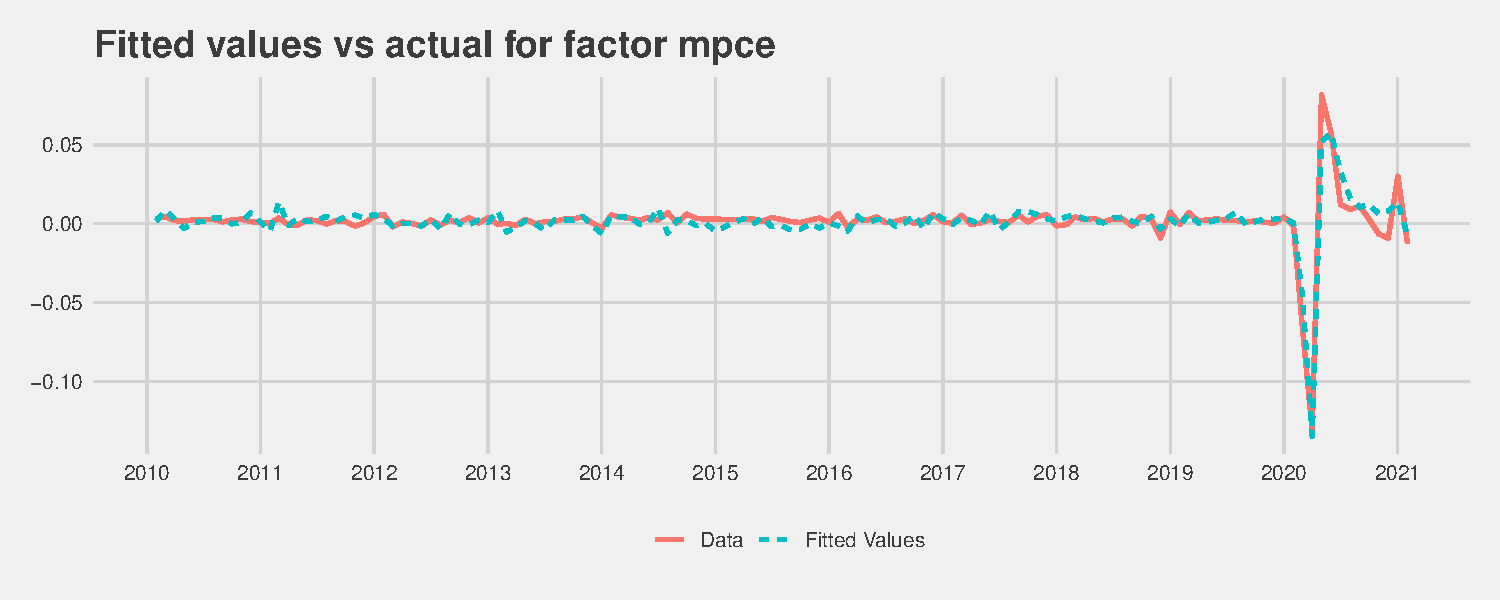
\includegraphics[width=5in,height=2in]{D:/Onedrive/__Projects/econforecasting/model-outputs/latex-figures/unnamed-chunk-25-1} 

}




{\centering 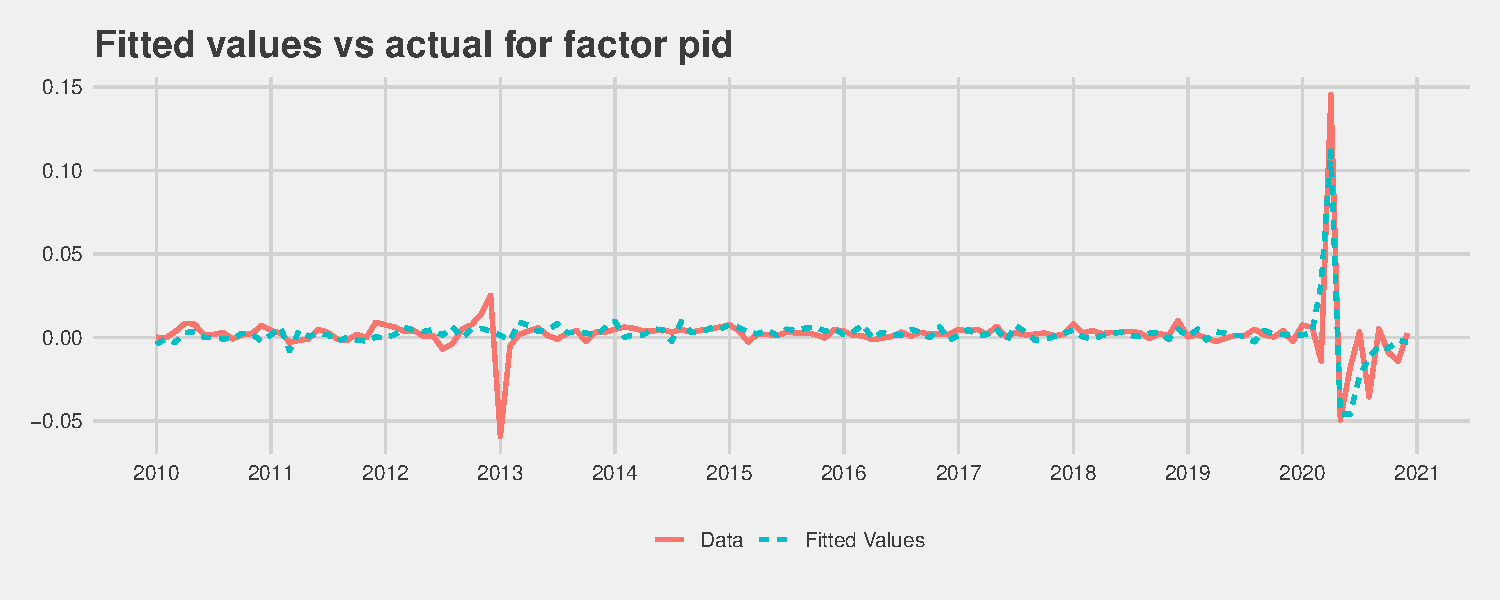
\includegraphics[width=5in,height=2in]{D:/Onedrive/__Projects/econforecasting/model-outputs/latex-figures/unnamed-chunk-25-2} 

}




{\centering 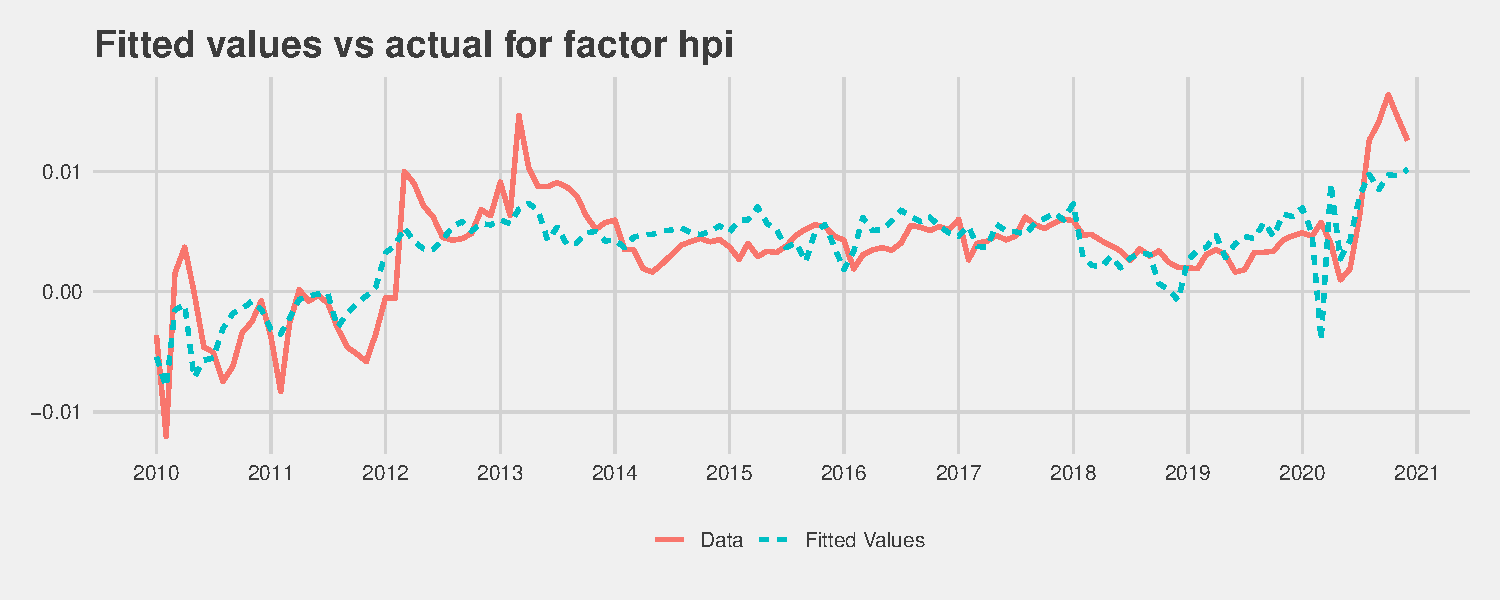
\includegraphics[width=5in,height=2in]{D:/Onedrive/__Projects/econforecasting/model-outputs/latex-figures/unnamed-chunk-25-3} 

}




{\centering 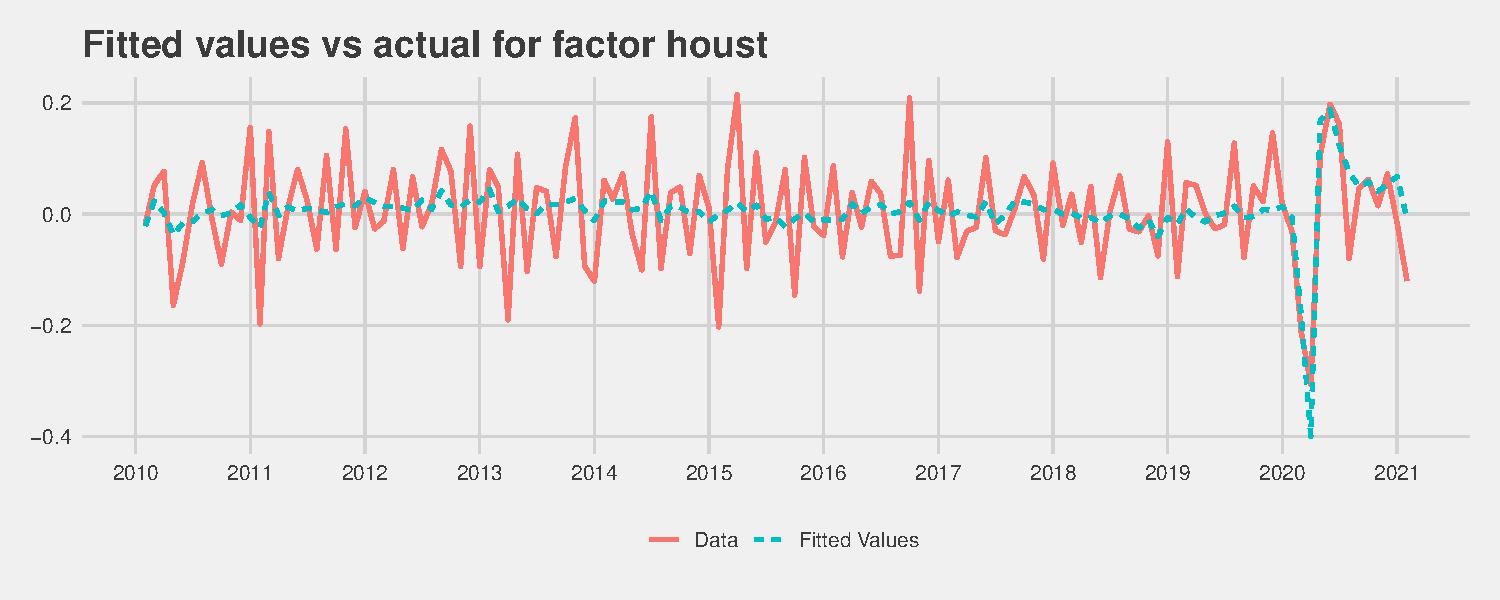
\includegraphics[width=5in,height=2in]{D:/Onedrive/__Projects/econforecasting/model-outputs/latex-figures/unnamed-chunk-25-4} 

}




{\centering 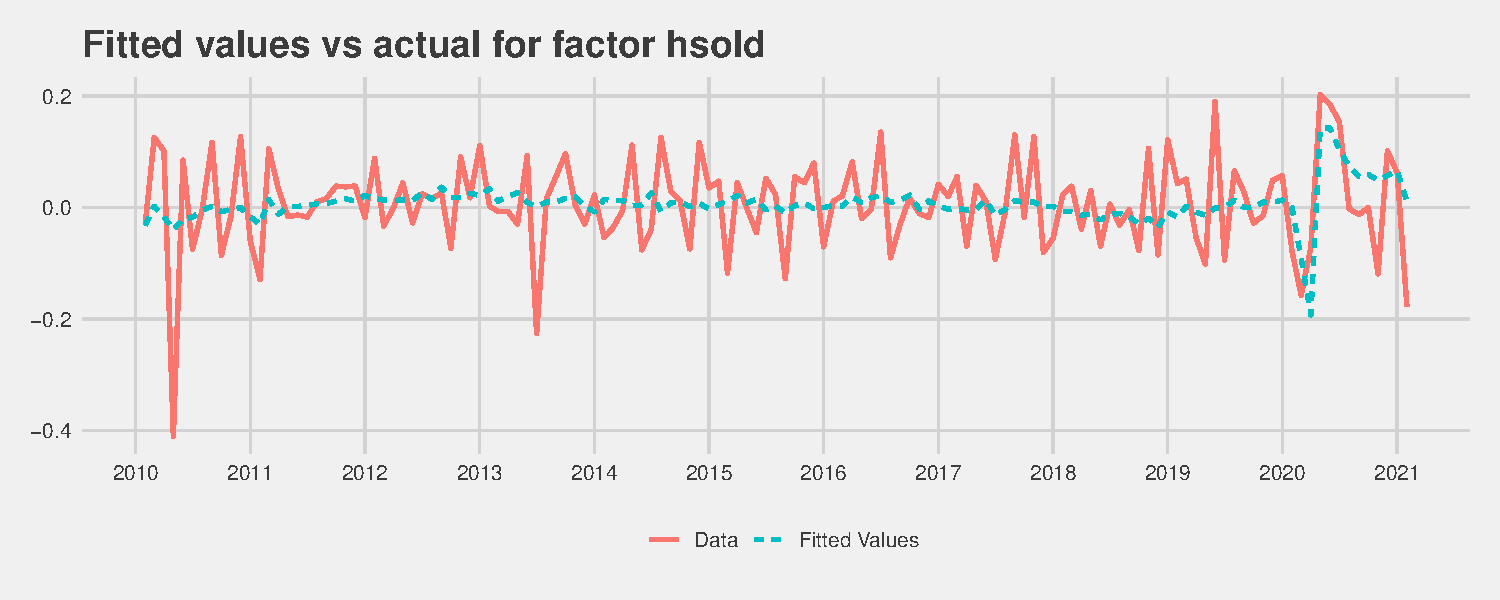
\includegraphics[width=5in,height=2in]{D:/Onedrive/__Projects/econforecasting/model-outputs/latex-figures/unnamed-chunk-25-5} 

}




{\centering 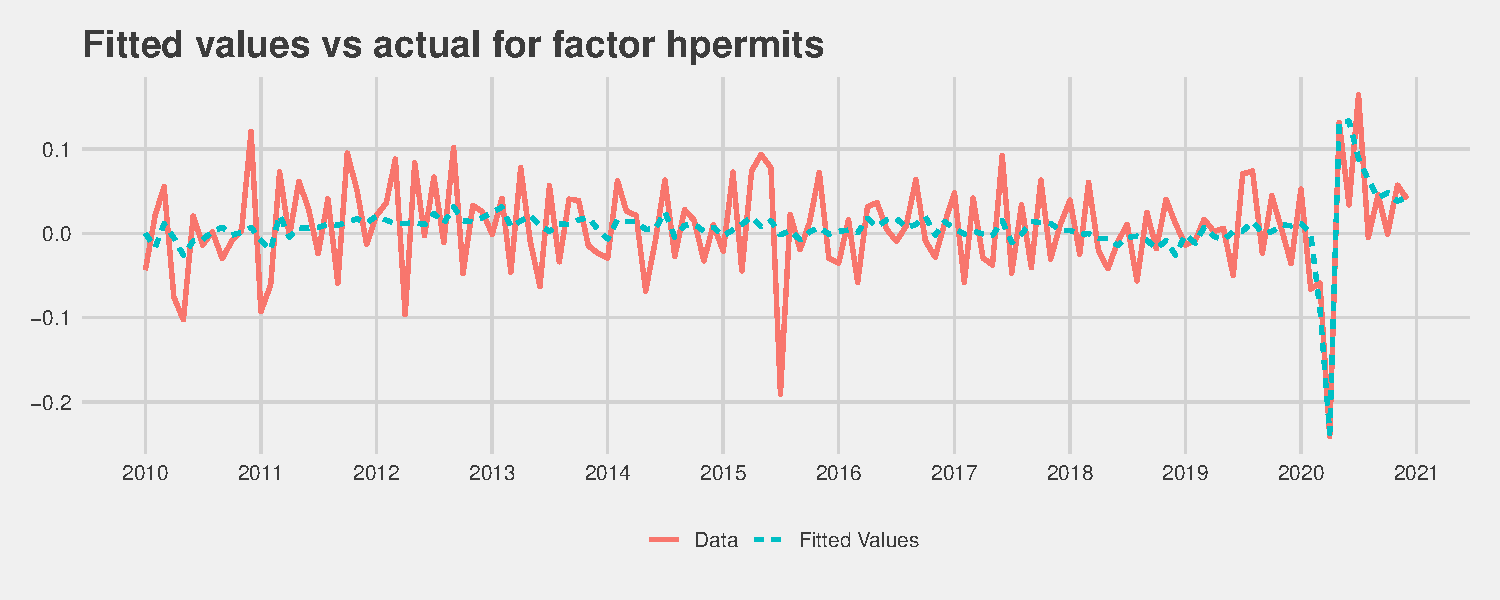
\includegraphics[width=5in,height=2in]{D:/Onedrive/__Projects/econforecasting/model-outputs/latex-figures/unnamed-chunk-25-6} 

}




{\centering 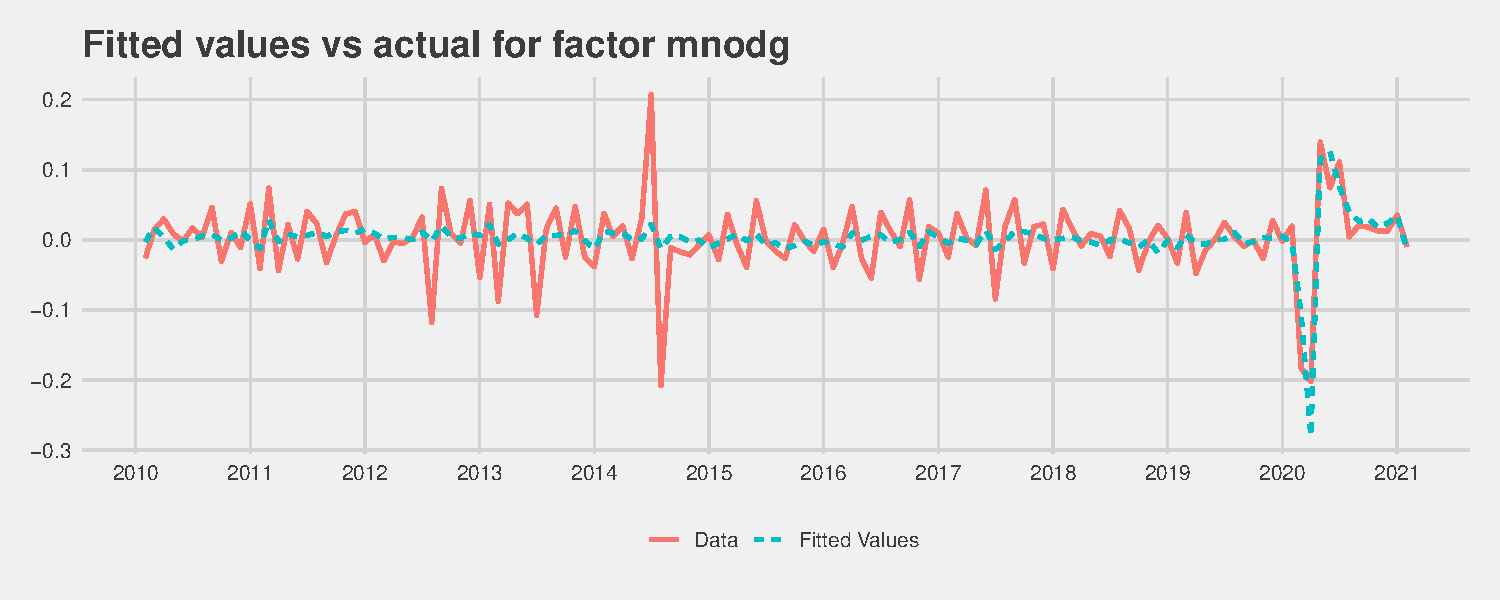
\includegraphics[width=5in,height=2in]{D:/Onedrive/__Projects/econforecasting/model-outputs/latex-figures/unnamed-chunk-25-7} 

}




{\centering 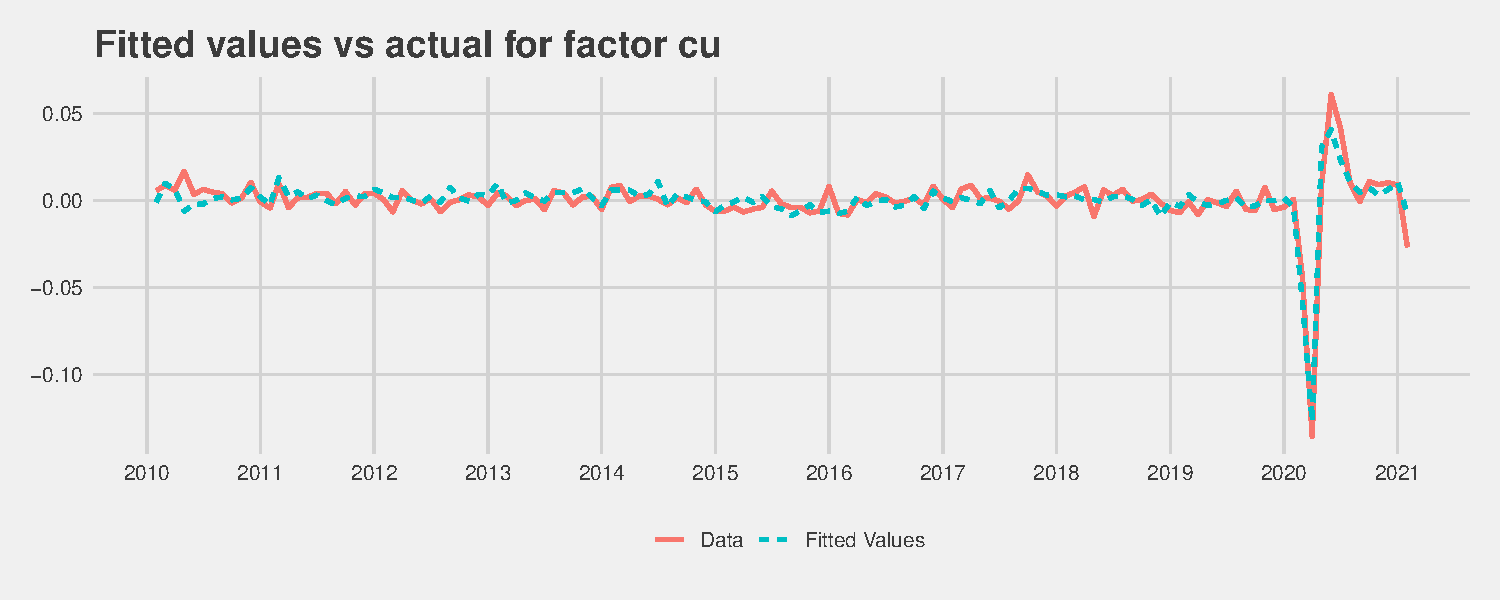
\includegraphics[width=5in,height=2in]{D:/Onedrive/__Projects/econforecasting/model-outputs/latex-figures/unnamed-chunk-25-8} 

}




{\centering 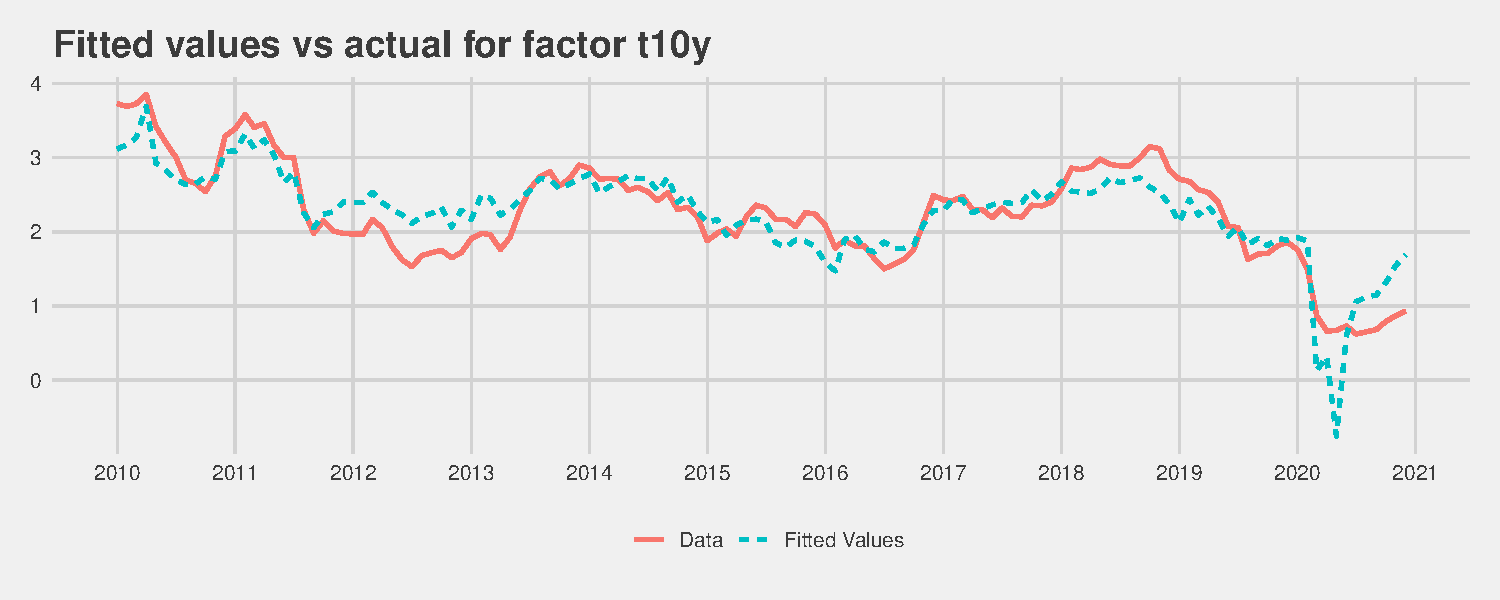
\includegraphics[width=5in,height=2in]{D:/Onedrive/__Projects/econforecasting/model-outputs/latex-figures/unnamed-chunk-25-9} 

}




{\centering 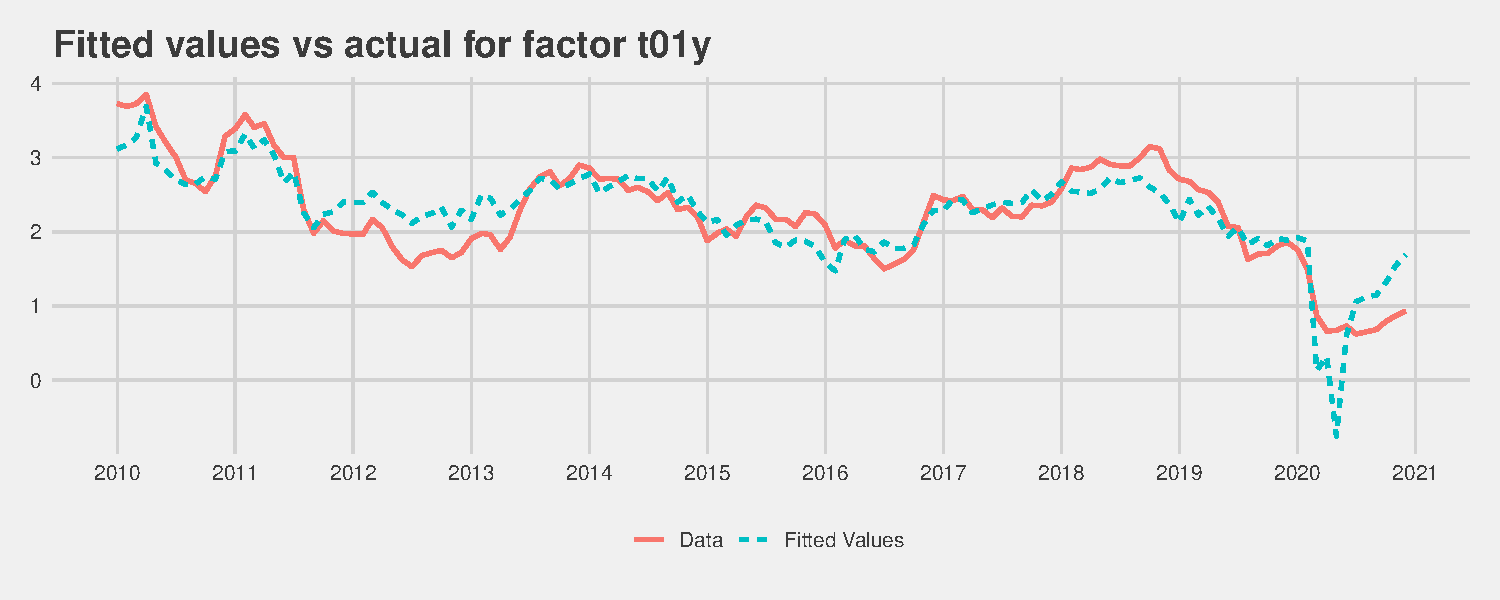
\includegraphics[width=5in,height=2in]{D:/Onedrive/__Projects/econforecasting/model-outputs/latex-figures/unnamed-chunk-25-10} 

}




{\centering 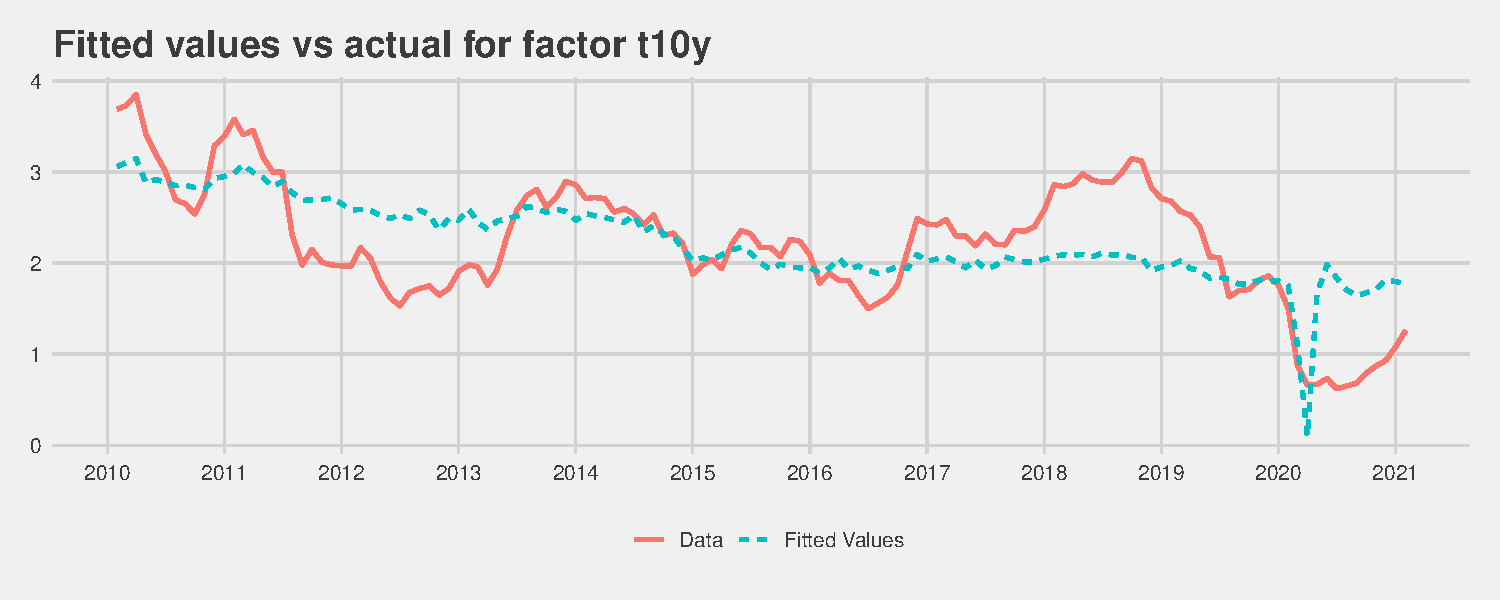
\includegraphics[width=5in,height=2in]{D:/Onedrive/__Projects/econforecasting/model-outputs/latex-figures/unnamed-chunk-25-11} 

}




{\centering 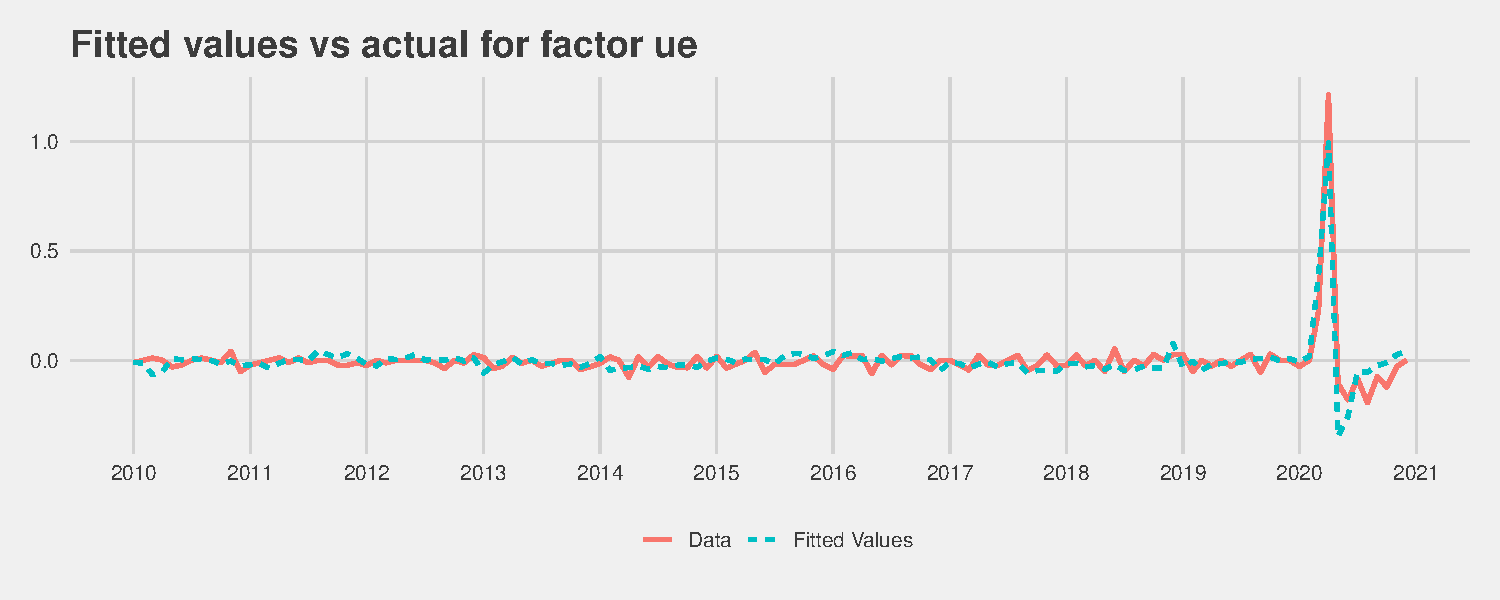
\includegraphics[width=5in,height=2in]{D:/Onedrive/__Projects/econforecasting/model-outputs/latex-figures/unnamed-chunk-25-12} 

}




{\centering 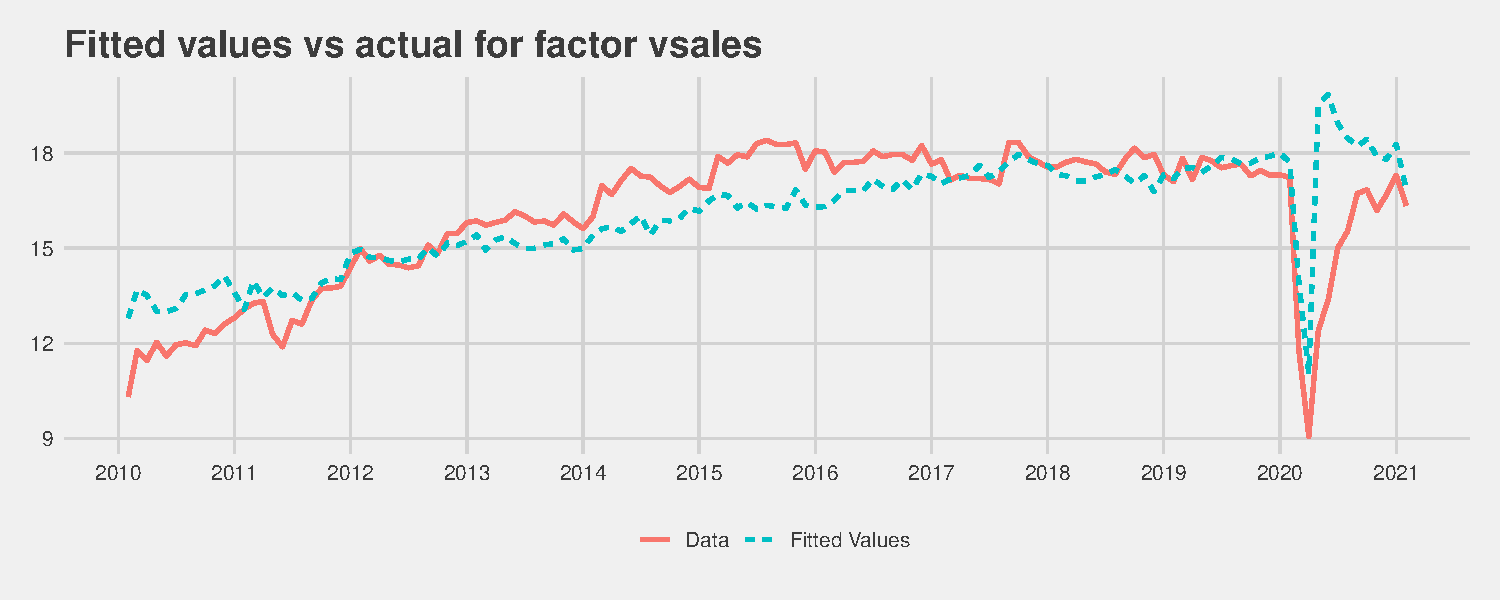
\includegraphics[width=5in,height=2in]{D:/Onedrive/__Projects/econforecasting/model-outputs/latex-figures/unnamed-chunk-25-13} 

}




{\centering 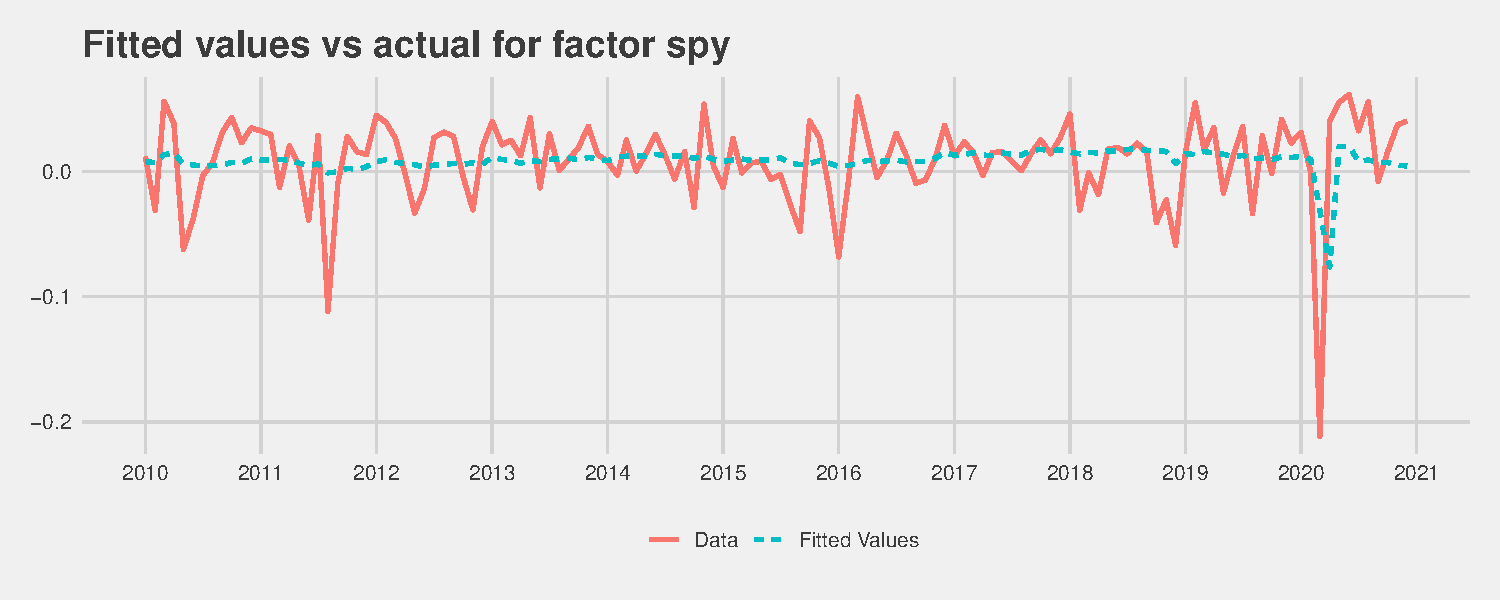
\includegraphics[width=5in,height=2in]{D:/Onedrive/__Projects/econforecasting/model-outputs/latex-figures/unnamed-chunk-25-14} 

}




{\centering 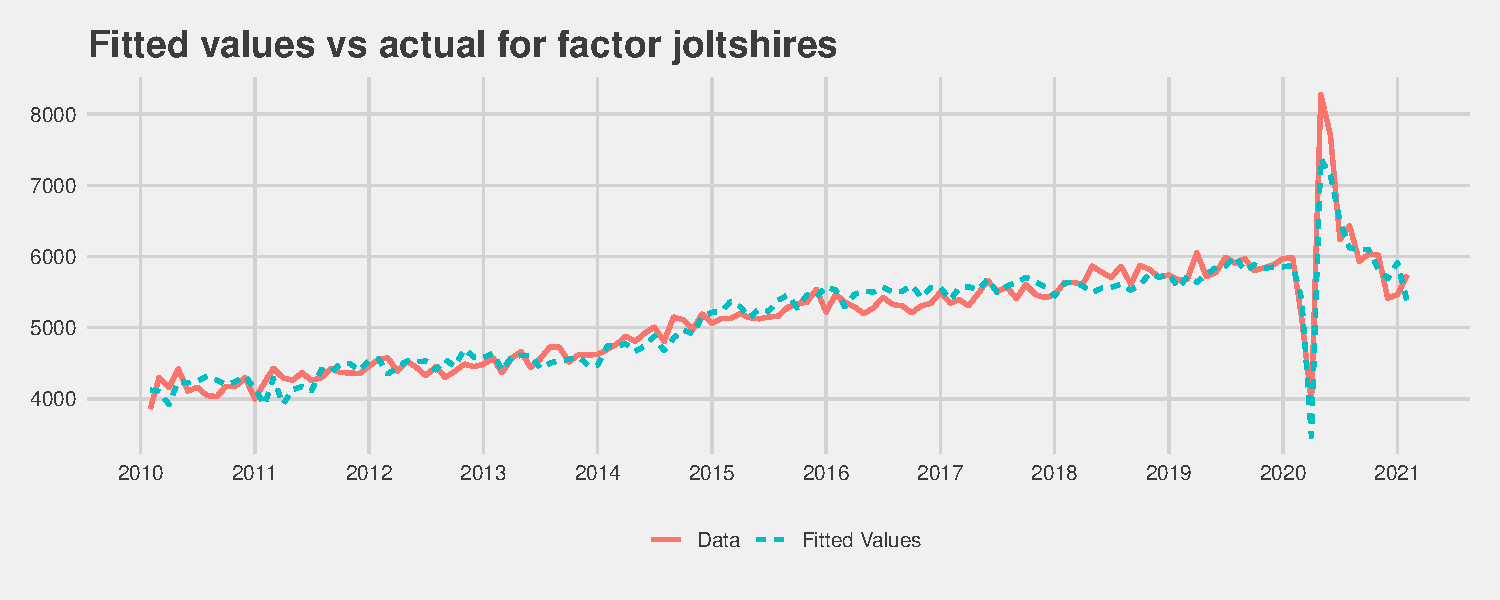
\includegraphics[width=5in,height=2in]{D:/Onedrive/__Projects/econforecasting/model-outputs/latex-figures/unnamed-chunk-25-15} 

}




{\centering 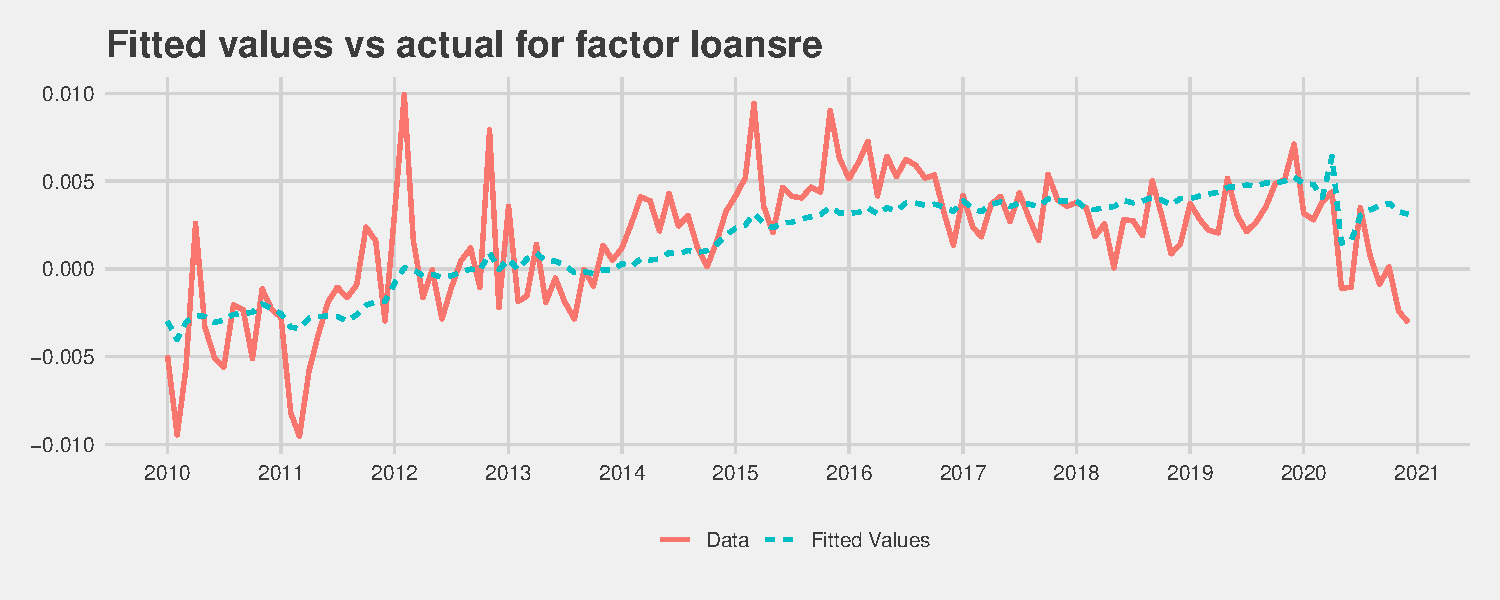
\includegraphics[width=5in,height=2in]{D:/Onedrive/__Projects/econforecasting/model-outputs/latex-figures/unnamed-chunk-25-16} 

}




{\centering 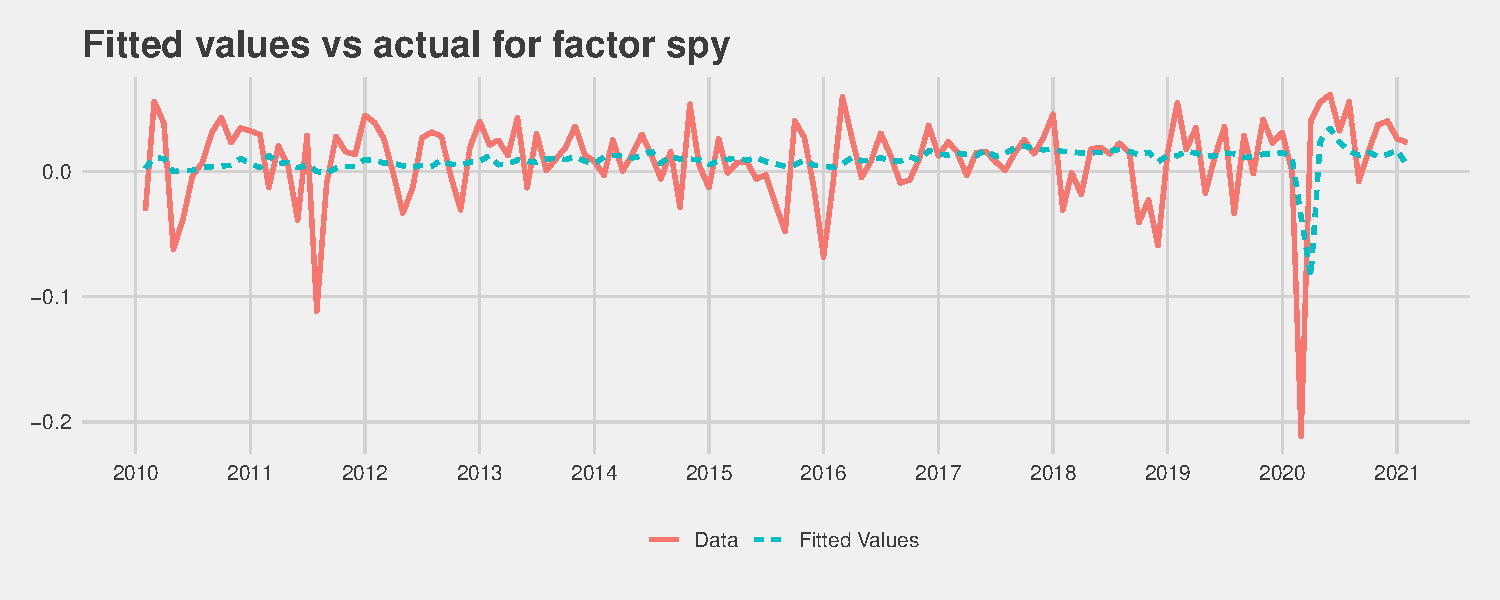
\includegraphics[width=5in,height=2in]{D:/Onedrive/__Projects/econforecasting/model-outputs/latex-figures/unnamed-chunk-25-17} 

}




{\centering 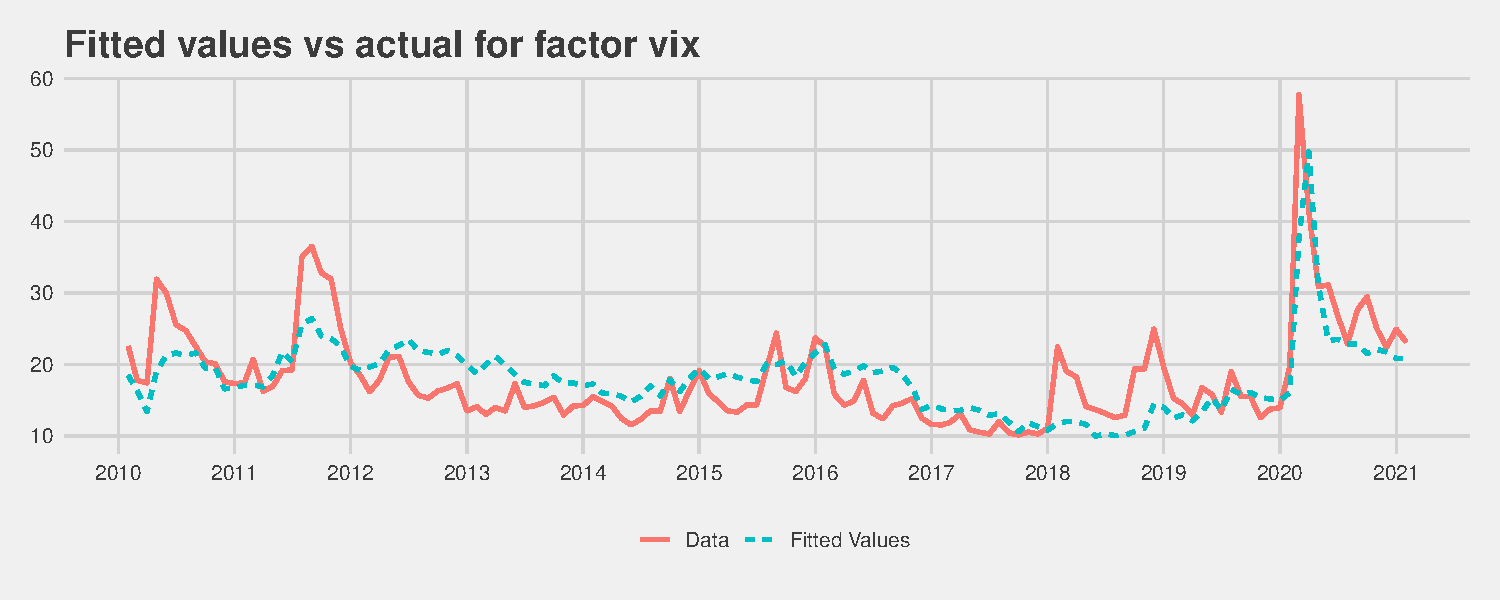
\includegraphics[width=5in,height=2in]{D:/Onedrive/__Projects/econforecasting/model-outputs/latex-figures/unnamed-chunk-25-18} 

}




{\centering 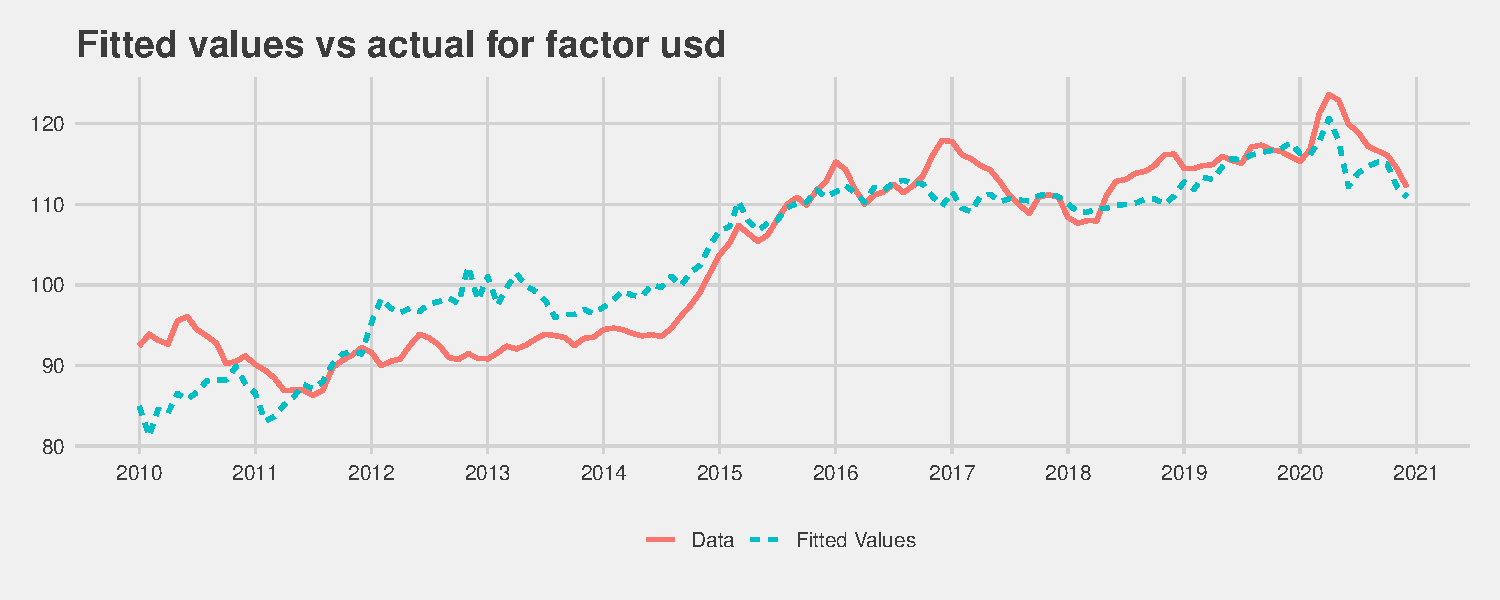
\includegraphics[width=5in,height=2in]{D:/Onedrive/__Projects/econforecasting/model-outputs/latex-figures/unnamed-chunk-25-19} 

}




{\centering 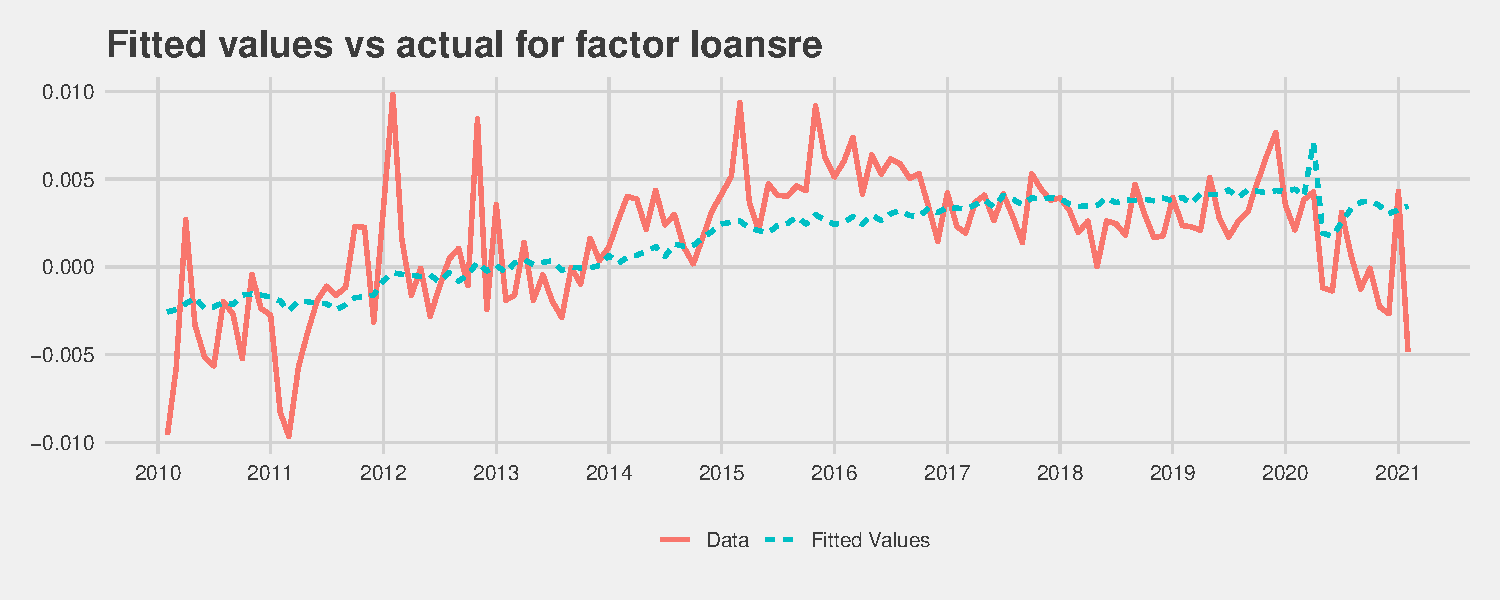
\includegraphics[width=5in,height=2in]{D:/Onedrive/__Projects/econforecasting/model-outputs/latex-figures/unnamed-chunk-25-20} 

}




{\centering 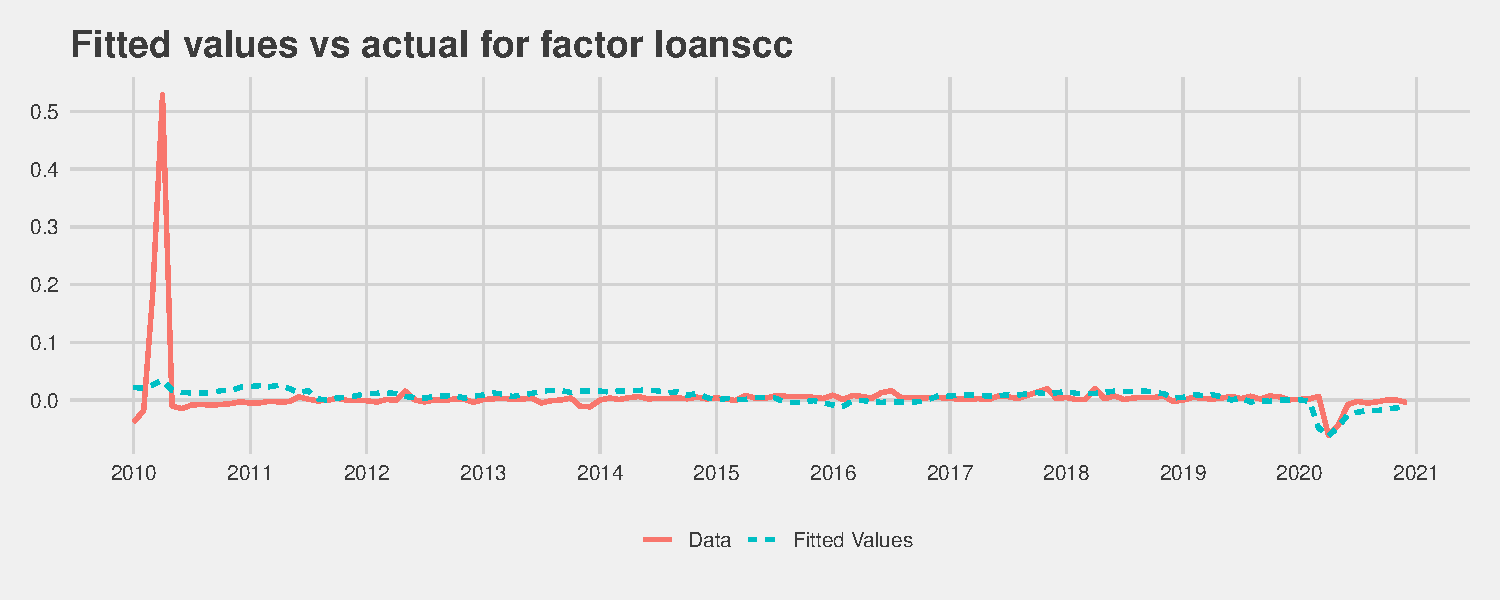
\includegraphics[width=5in,height=2in]{D:/Onedrive/__Projects/econforecasting/model-outputs/latex-figures/unnamed-chunk-25-21} 

}




{\centering 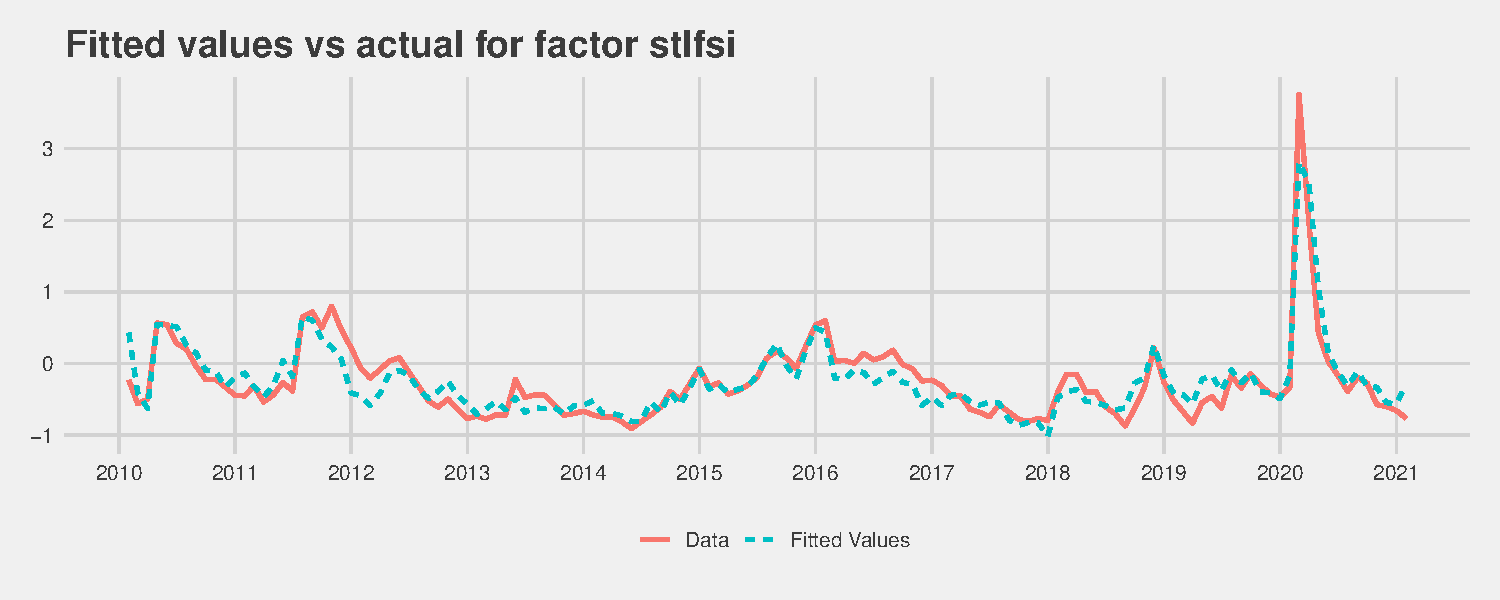
\includegraphics[width=5in,height=2in]{D:/Onedrive/__Projects/econforecasting/model-outputs/latex-figures/unnamed-chunk-25-22} 

}




{\centering 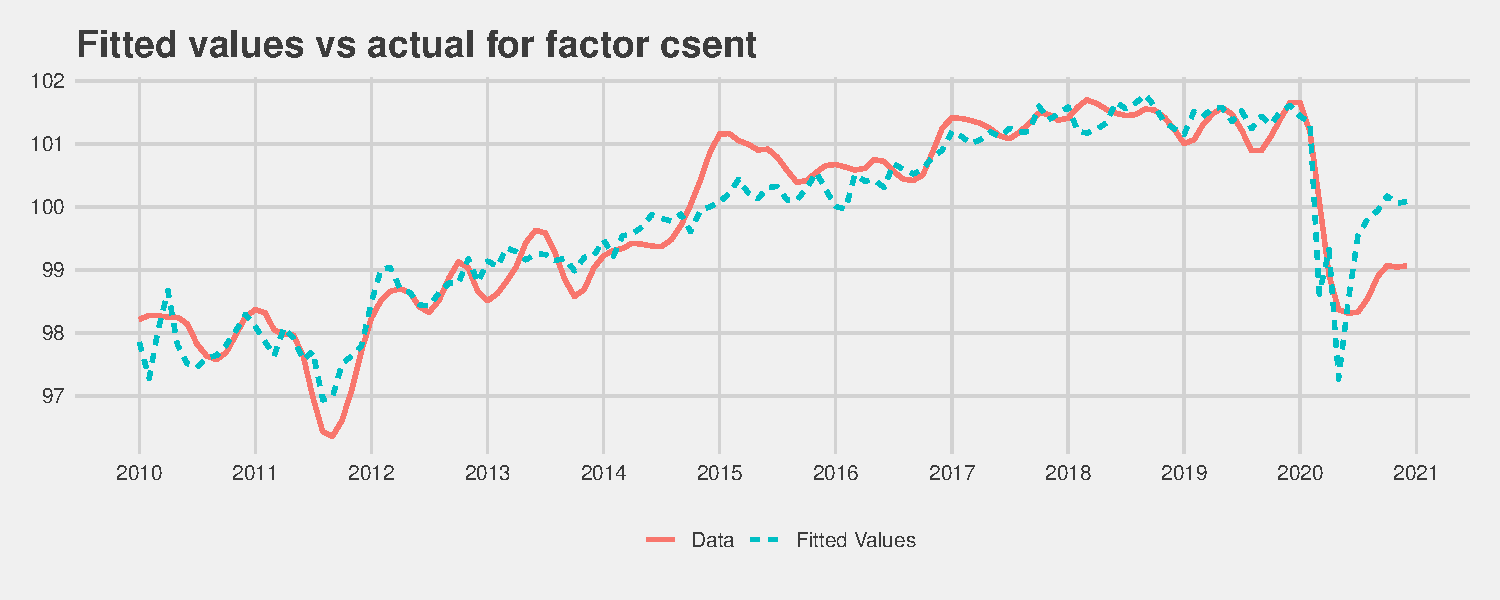
\includegraphics[width=5in,height=2in]{D:/Onedrive/__Projects/econforecasting/model-outputs/latex-figures/unnamed-chunk-25-23} 

}




{\centering 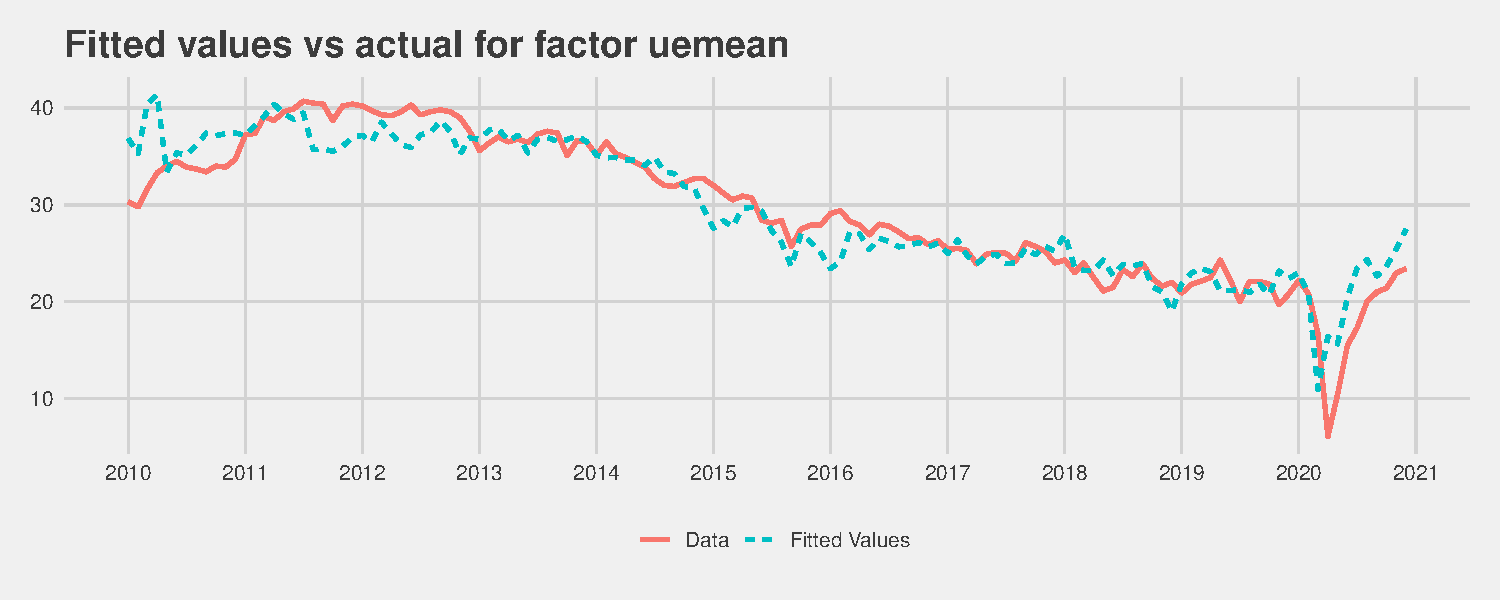
\includegraphics[width=5in,height=2in]{D:/Onedrive/__Projects/econforecasting/model-outputs/latex-figures/unnamed-chunk-25-24} 

}




{\centering 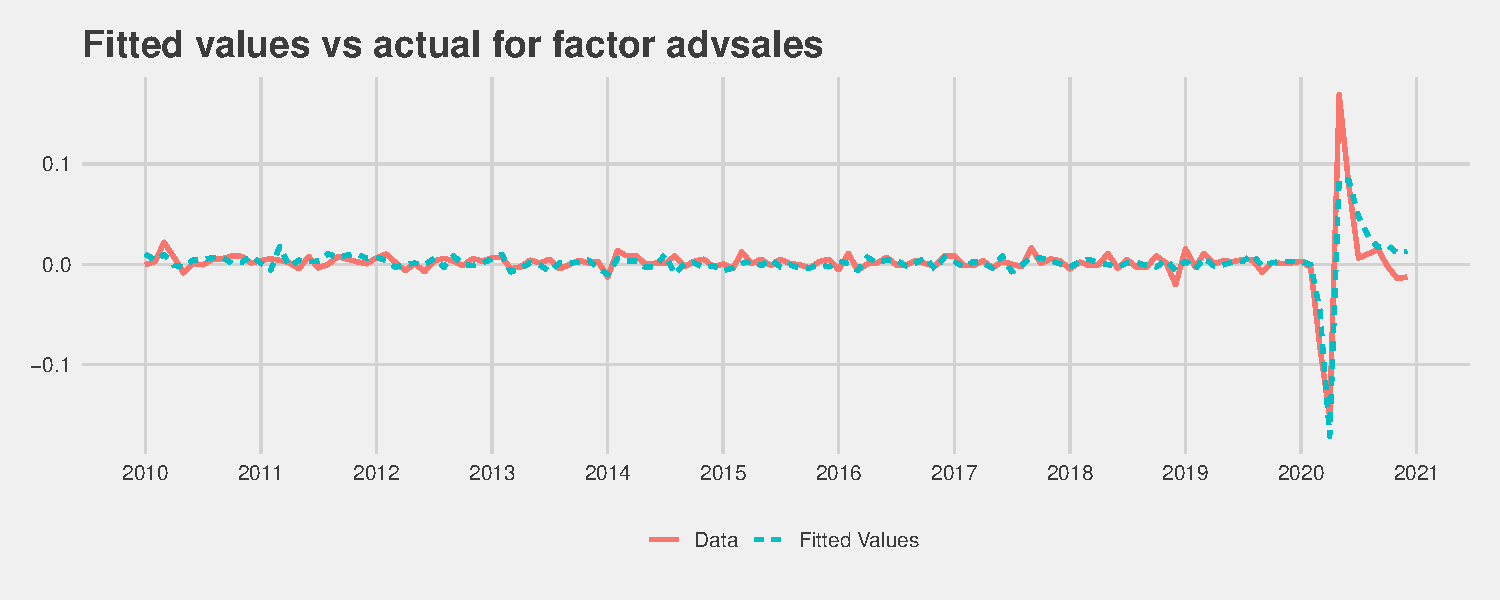
\includegraphics[width=5in,height=2in]{D:/Onedrive/__Projects/econforecasting/model-outputs/latex-figures/unnamed-chunk-25-25} 

}




{\centering 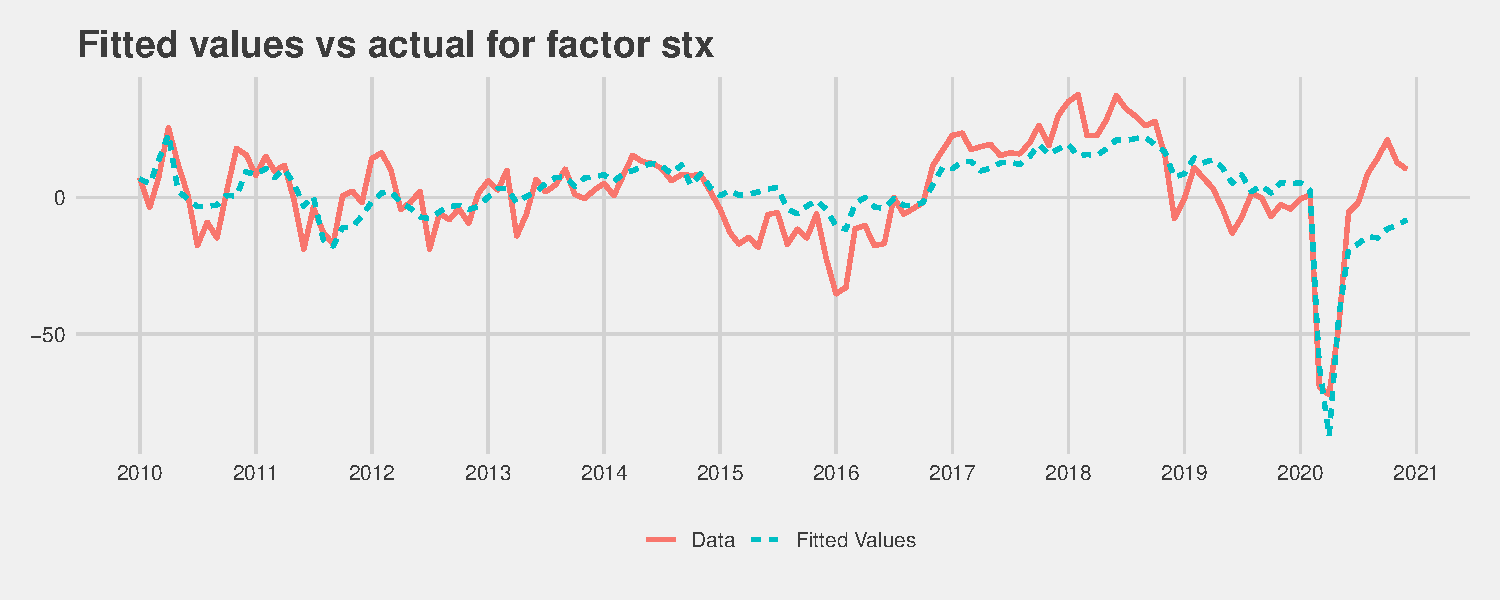
\includegraphics[width=5in,height=2in]{D:/Onedrive/__Projects/econforecasting/model-outputs/latex-figures/unnamed-chunk-25-26} 

}




{\centering 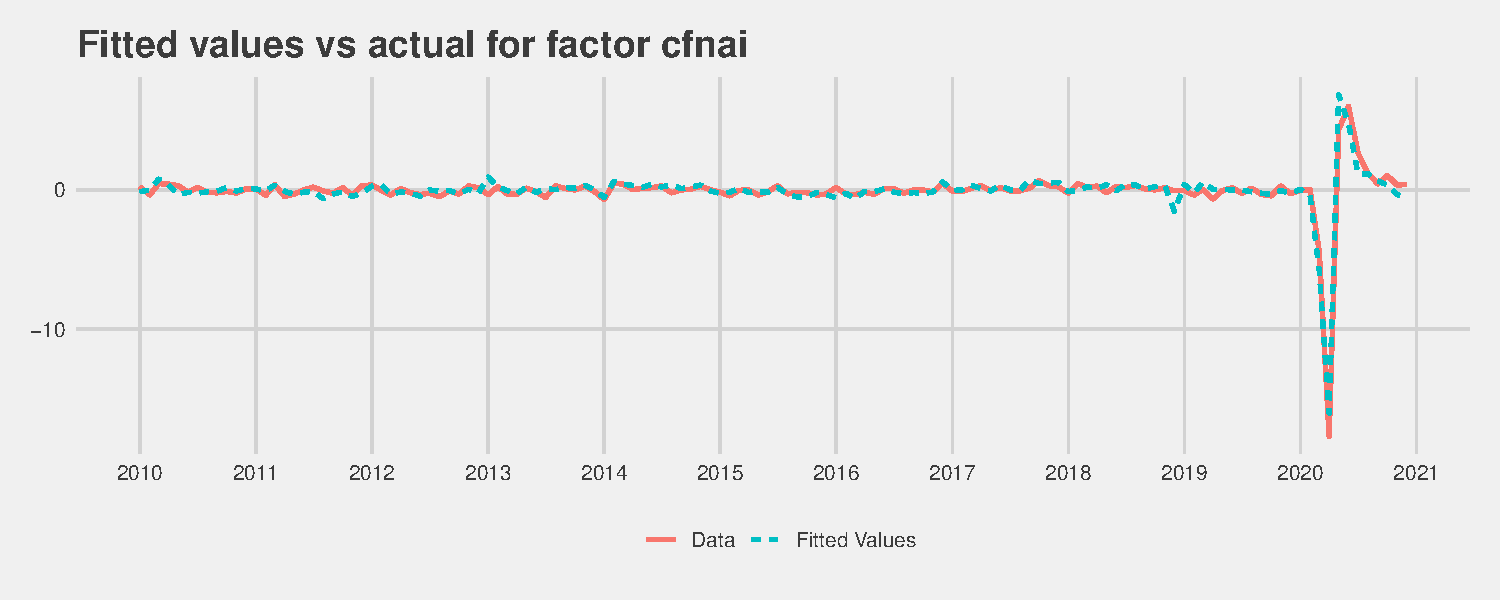
\includegraphics[width=5in,height=2in]{D:/Onedrive/__Projects/econforecasting/model-outputs/latex-figures/unnamed-chunk-25-27} 

}




{\centering 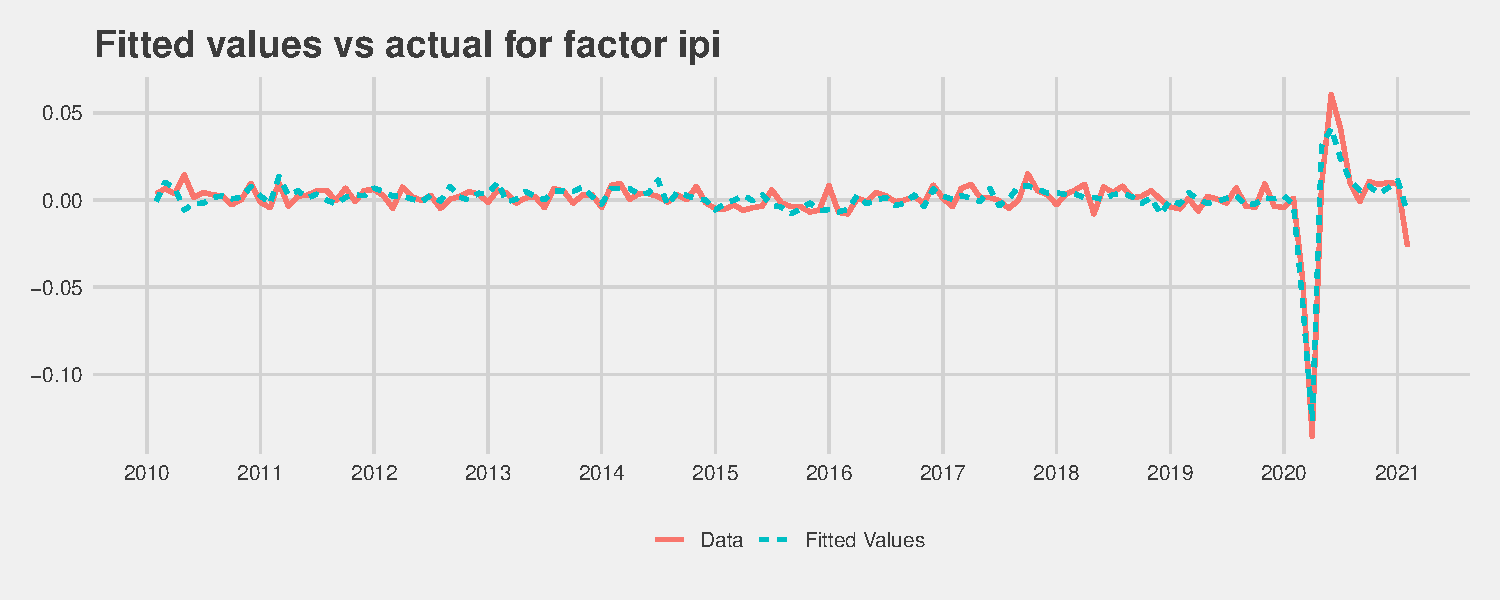
\includegraphics[width=5in,height=2in]{D:/Onedrive/__Projects/econforecasting/model-outputs/latex-figures/unnamed-chunk-25-28} 

}




{\centering 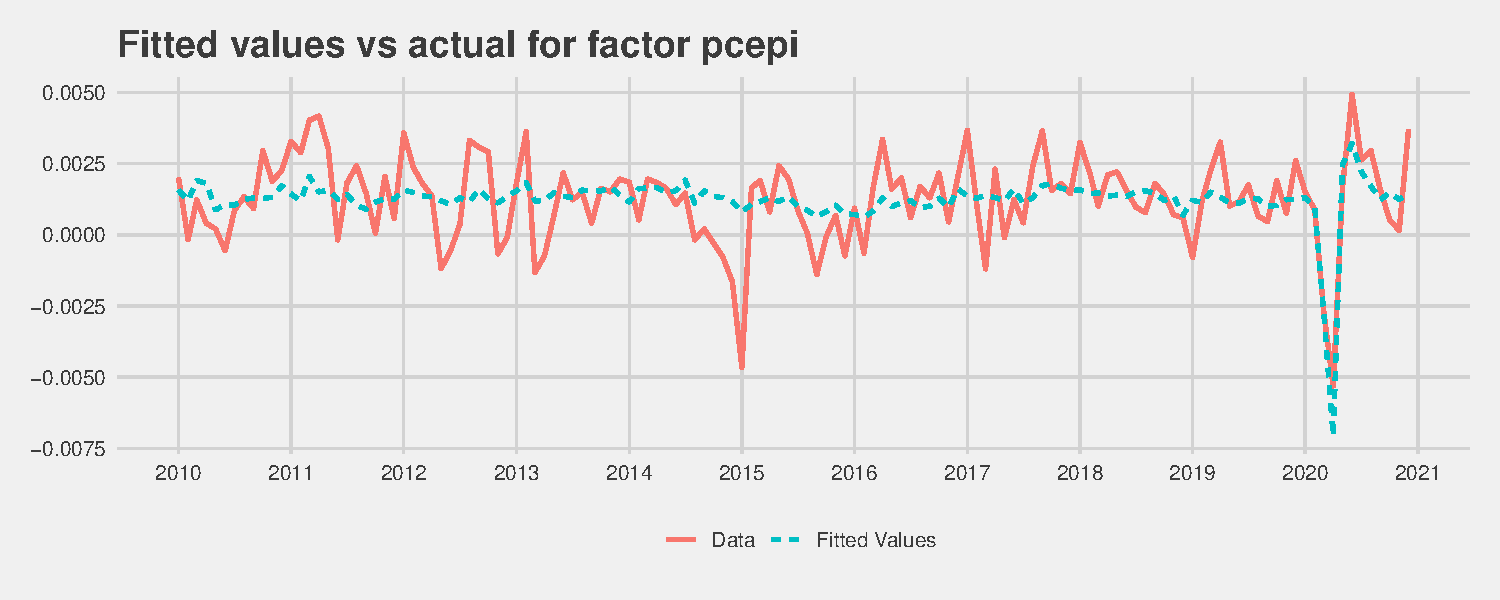
\includegraphics[width=5in,height=2in]{D:/Onedrive/__Projects/econforecasting/model-outputs/latex-figures/unnamed-chunk-25-29} 

}




{\centering 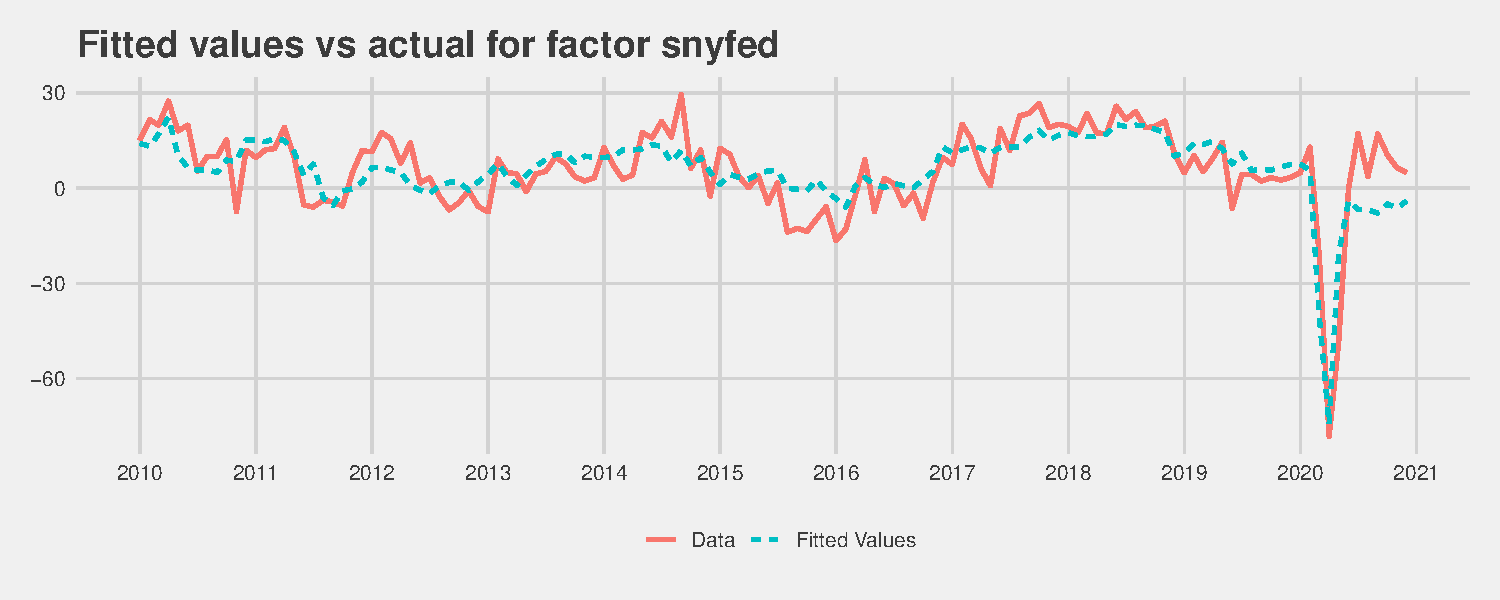
\includegraphics[width=5in,height=2in]{D:/Onedrive/__Projects/econforecasting/model-outputs/latex-figures/unnamed-chunk-25-30} 

}




{\centering 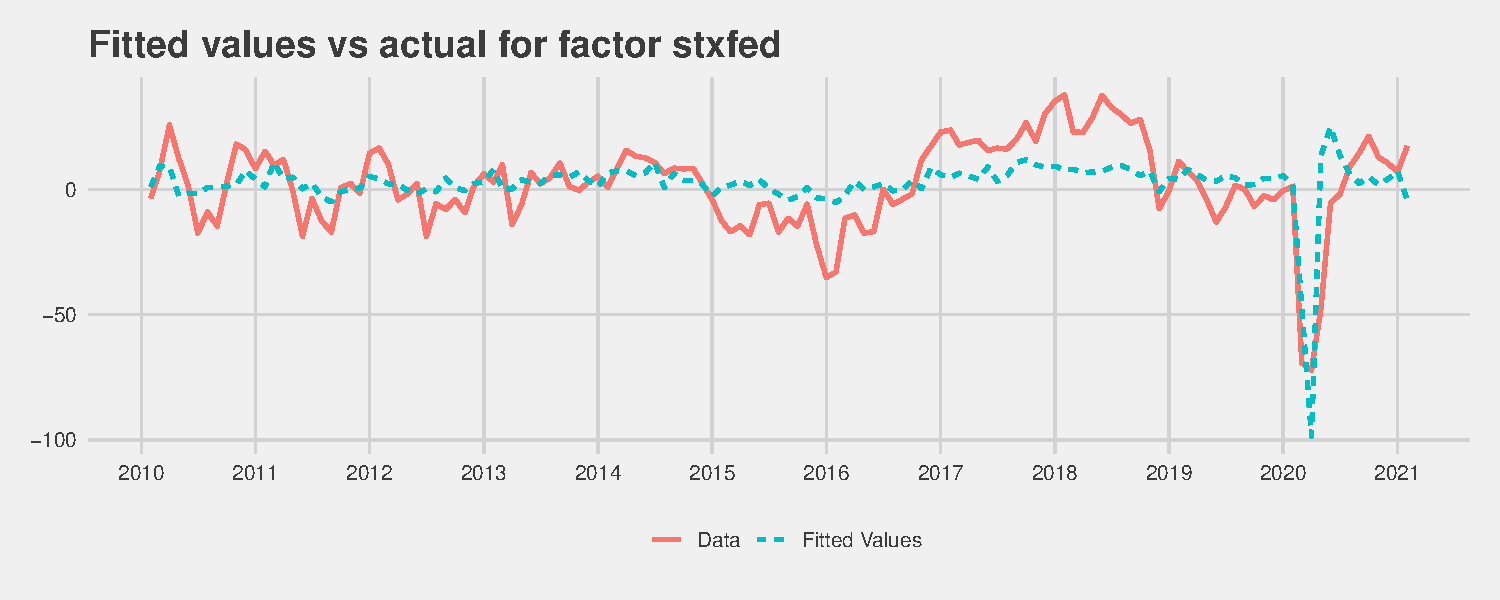
\includegraphics[width=5in,height=2in]{D:/Onedrive/__Projects/econforecasting/model-outputs/latex-figures/unnamed-chunk-25-31} 

}




{\centering 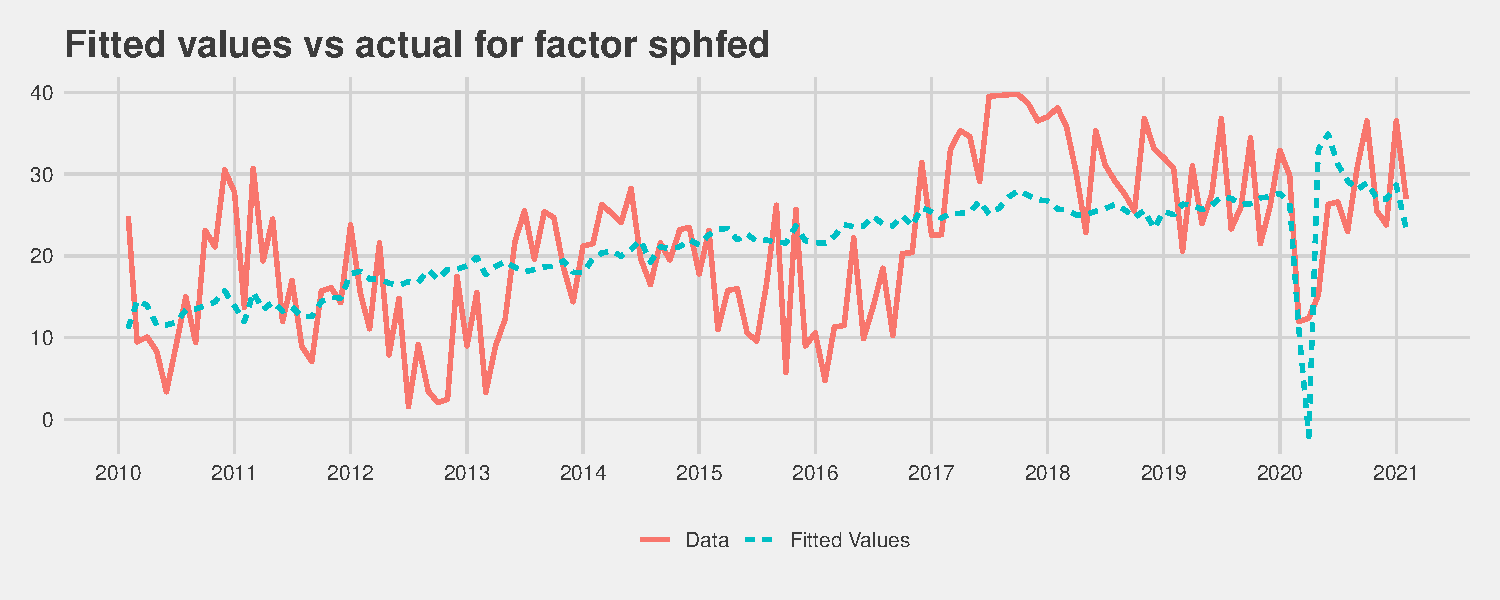
\includegraphics[width=5in,height=2in]{D:/Onedrive/__Projects/econforecasting/model-outputs/latex-figures/unnamed-chunk-25-32} 

}




{\centering 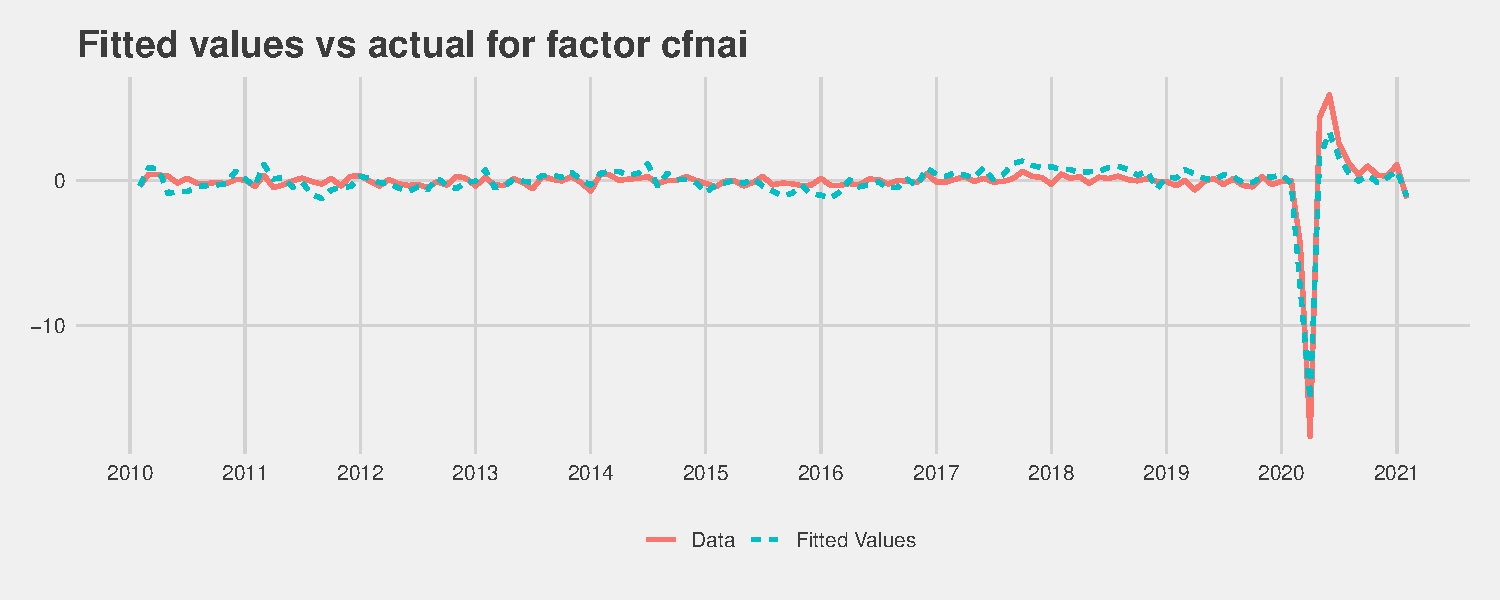
\includegraphics[width=5in,height=2in]{D:/Onedrive/__Projects/econforecasting/model-outputs/latex-figures/unnamed-chunk-25-33} 

}




{\centering 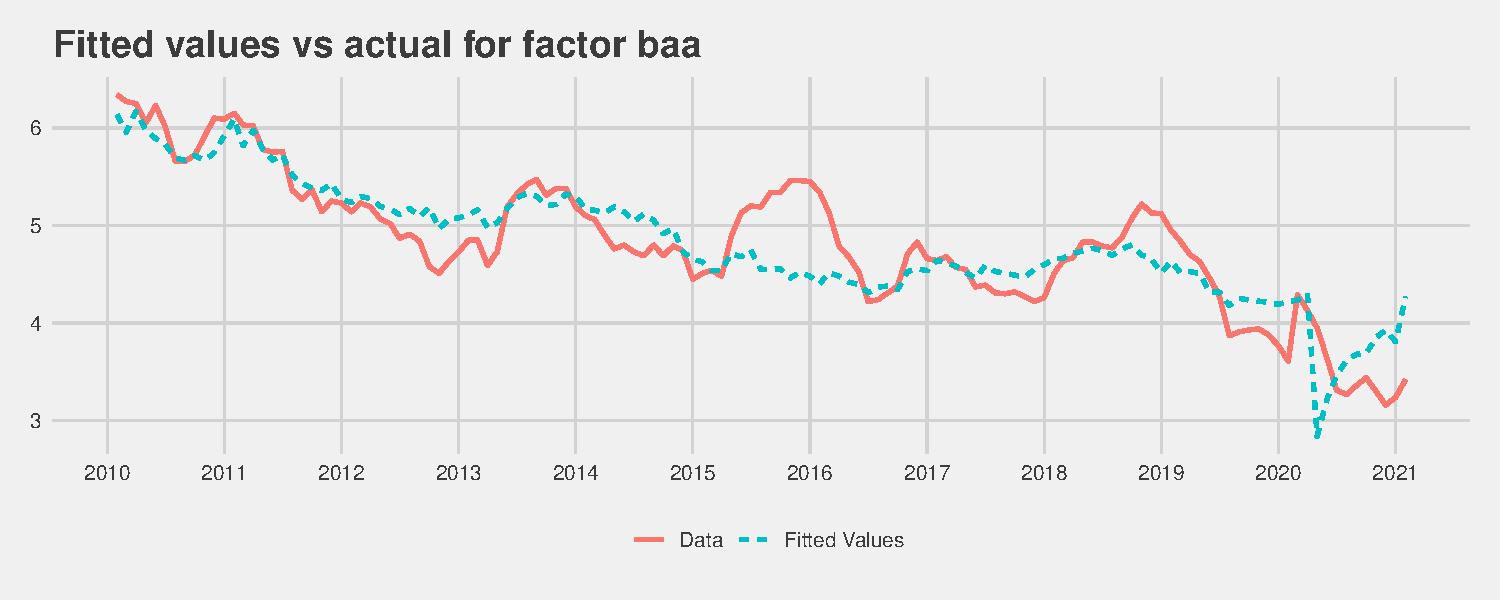
\includegraphics[width=5in,height=2in]{D:/Onedrive/__Projects/econforecasting/model-outputs/latex-figures/unnamed-chunk-25-34} 

}




{\centering 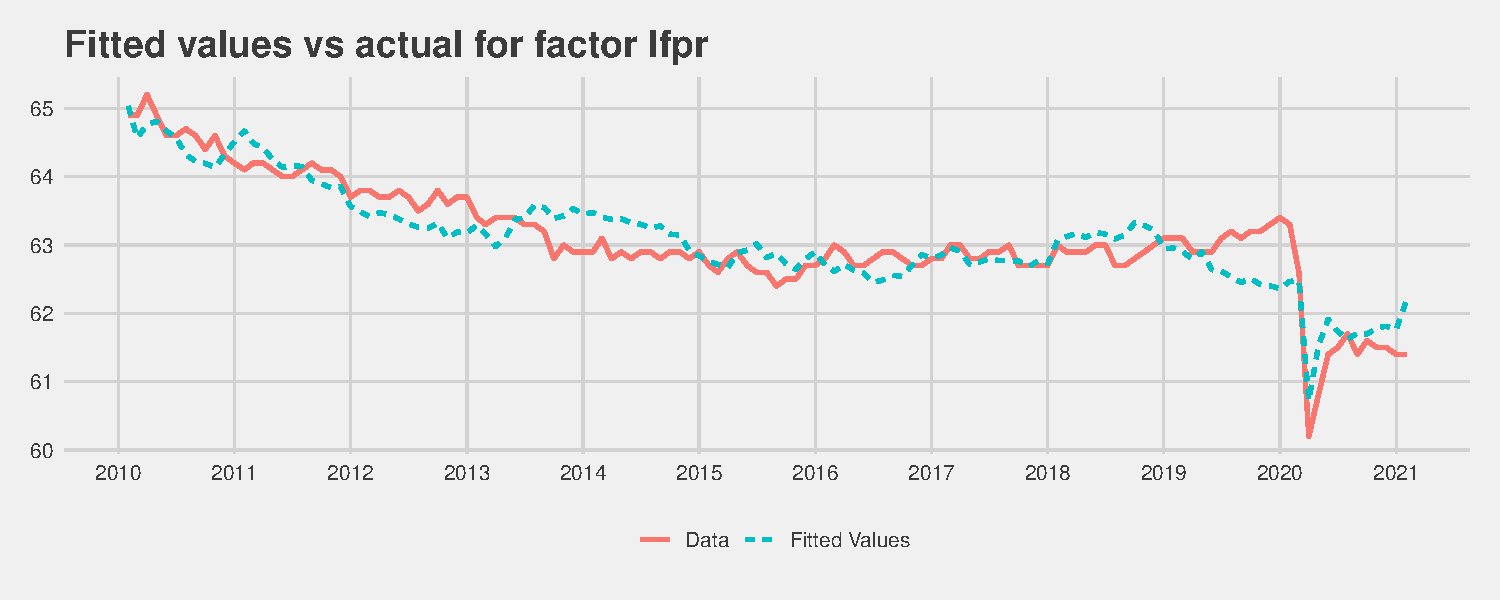
\includegraphics[width=5in,height=2in]{D:/Onedrive/__Projects/econforecasting/model-outputs/latex-figures/unnamed-chunk-25-35} 

}





\end{document}
